
% In the following figures, the t-SNE results of different perplexitites are compared, for the different time length files (1h and 3h), using the first columns of each feature (1h: first 15 minutes, 3h: fist 30 minutes ). The left scatter plots depict t-SNE results, the right scatter plots visualise DBSCAN clusterings of t-SNE results).

%------------------ LEARNING RATE 10: ------------------
\subsubsection{Learning Rate = 10}
% -- 1h, lr 10 --
\begin{figure}[H]
  \centering
  \begin{subfigure}{.5\textwidth}
    \centering
    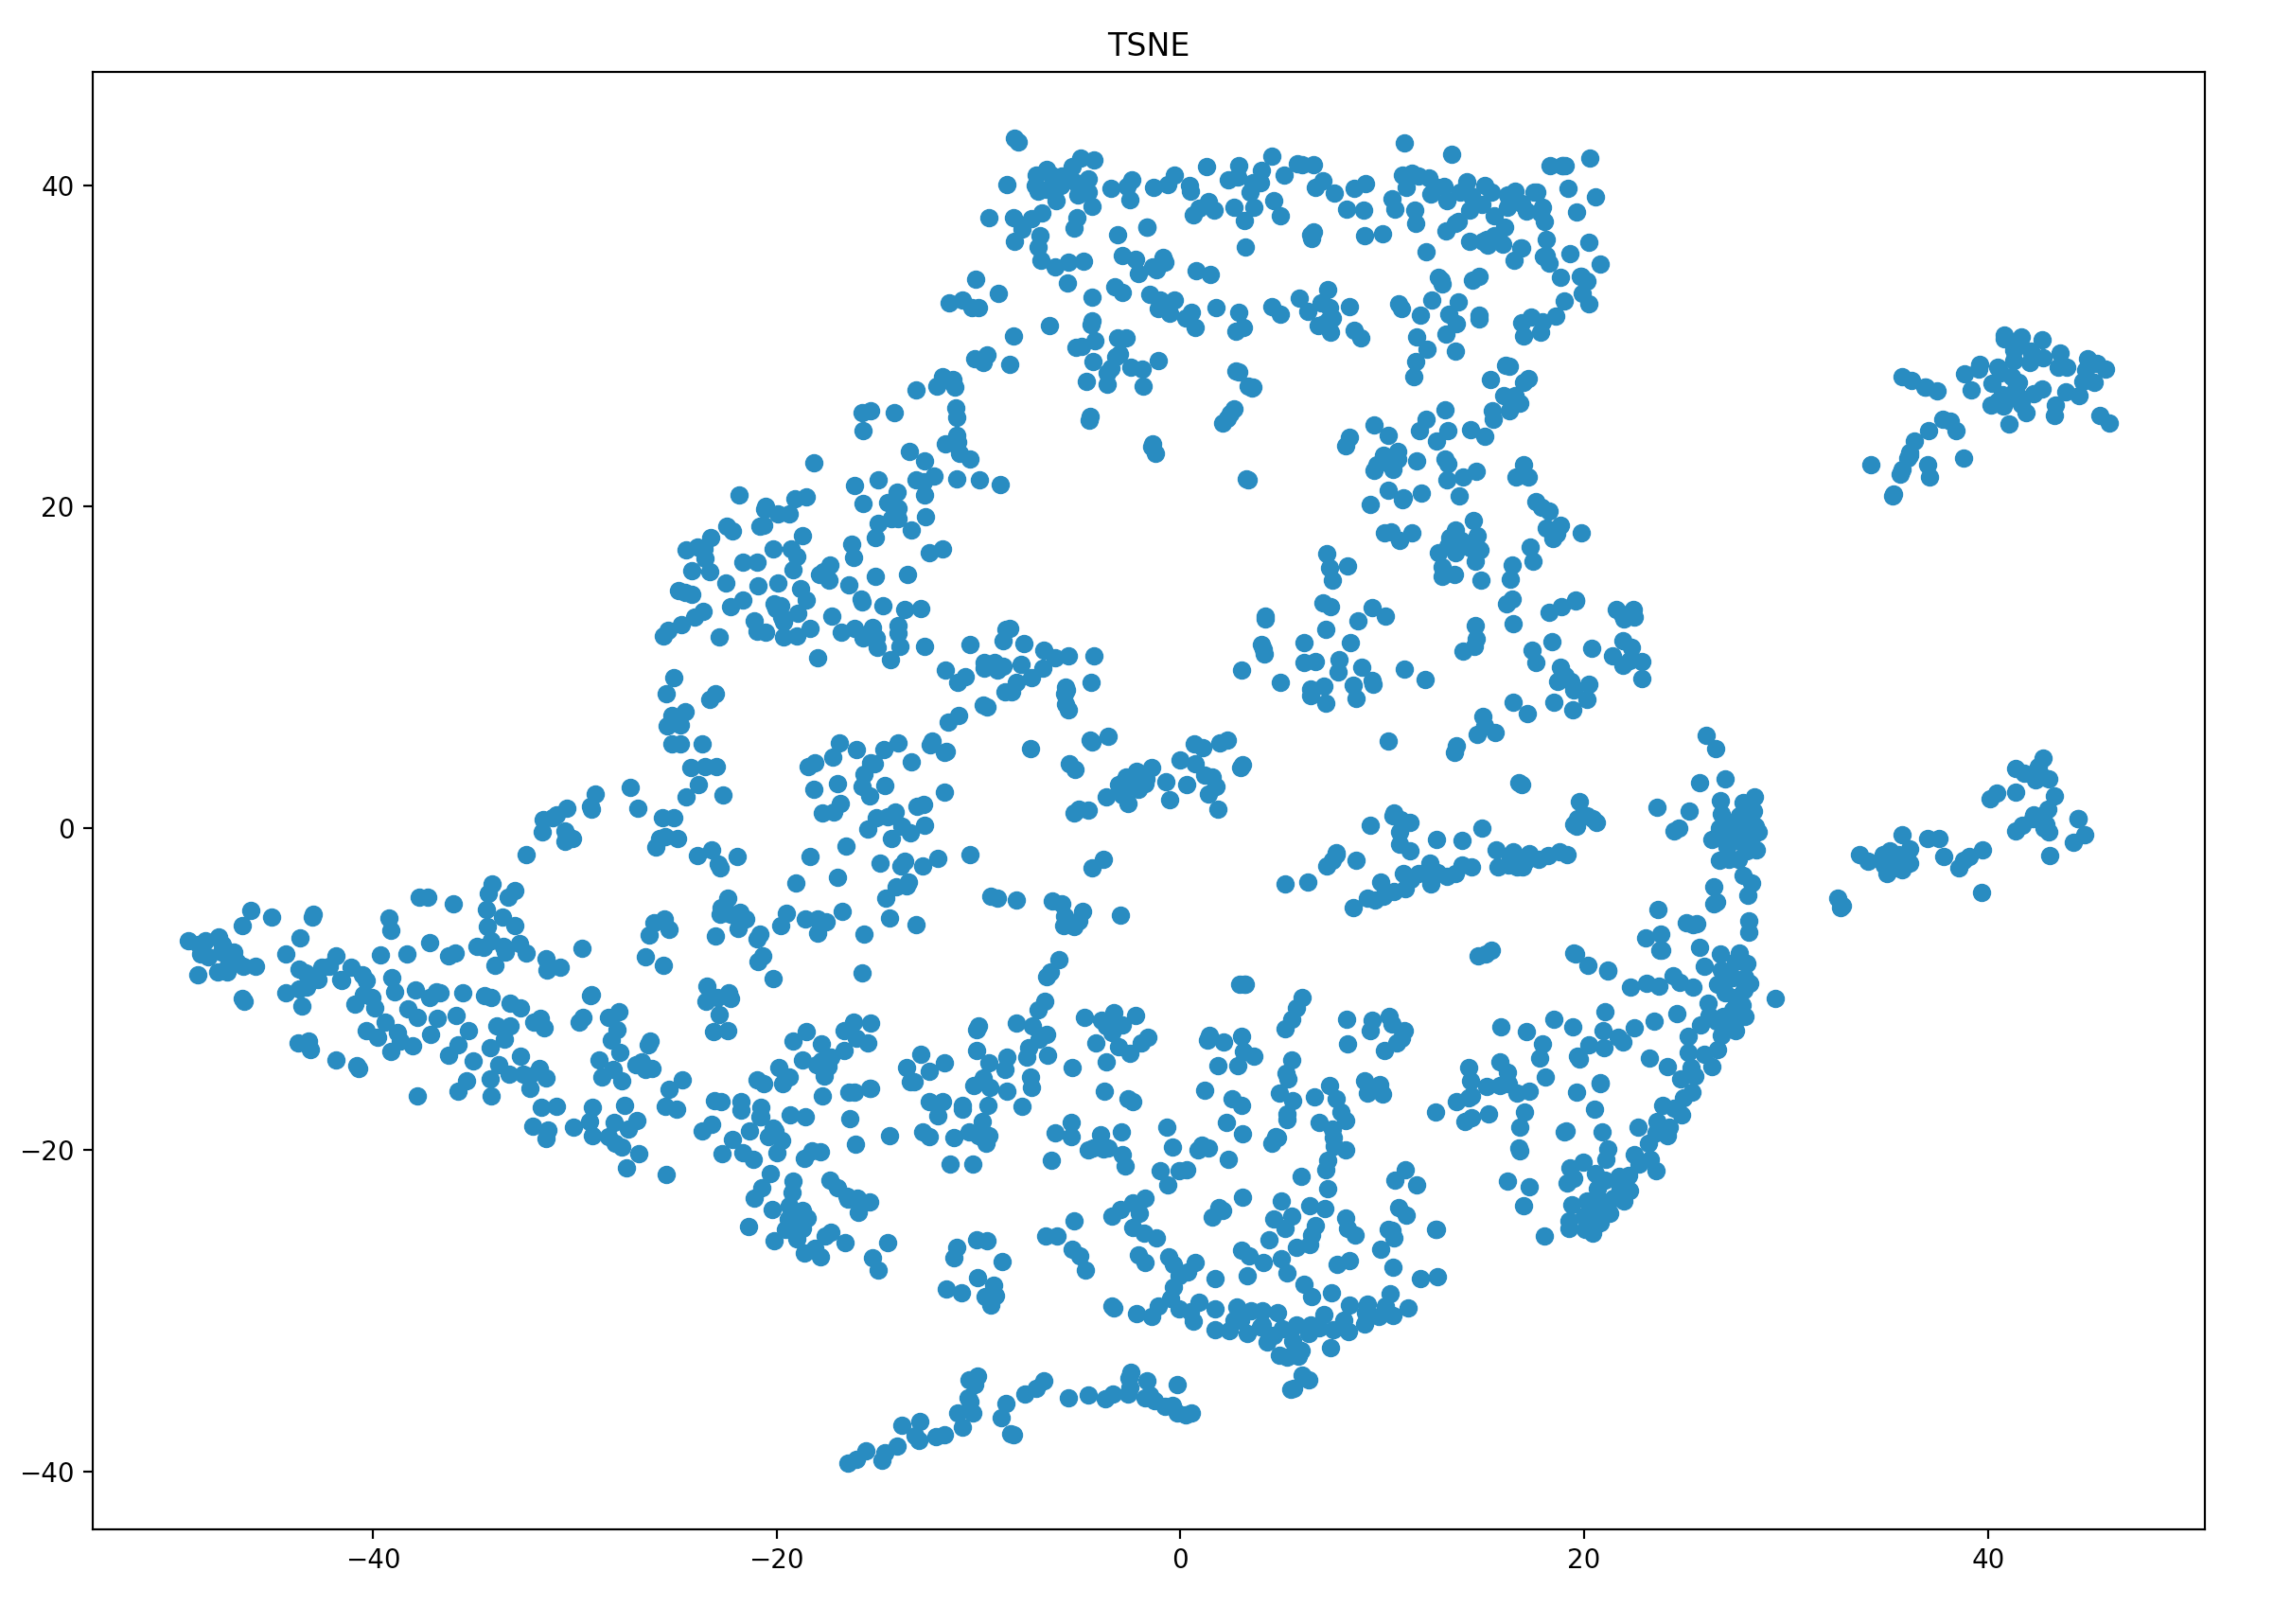
\includegraphics[width=0.9\textwidth]{./images/tsneParametersTest/learningRate/lr10-1hTSNE.png}
  % \caption{}
  % \label{figure:}
  \end{subfigure}%
  \begin{subfigure}{.5\textwidth}
    \centering
    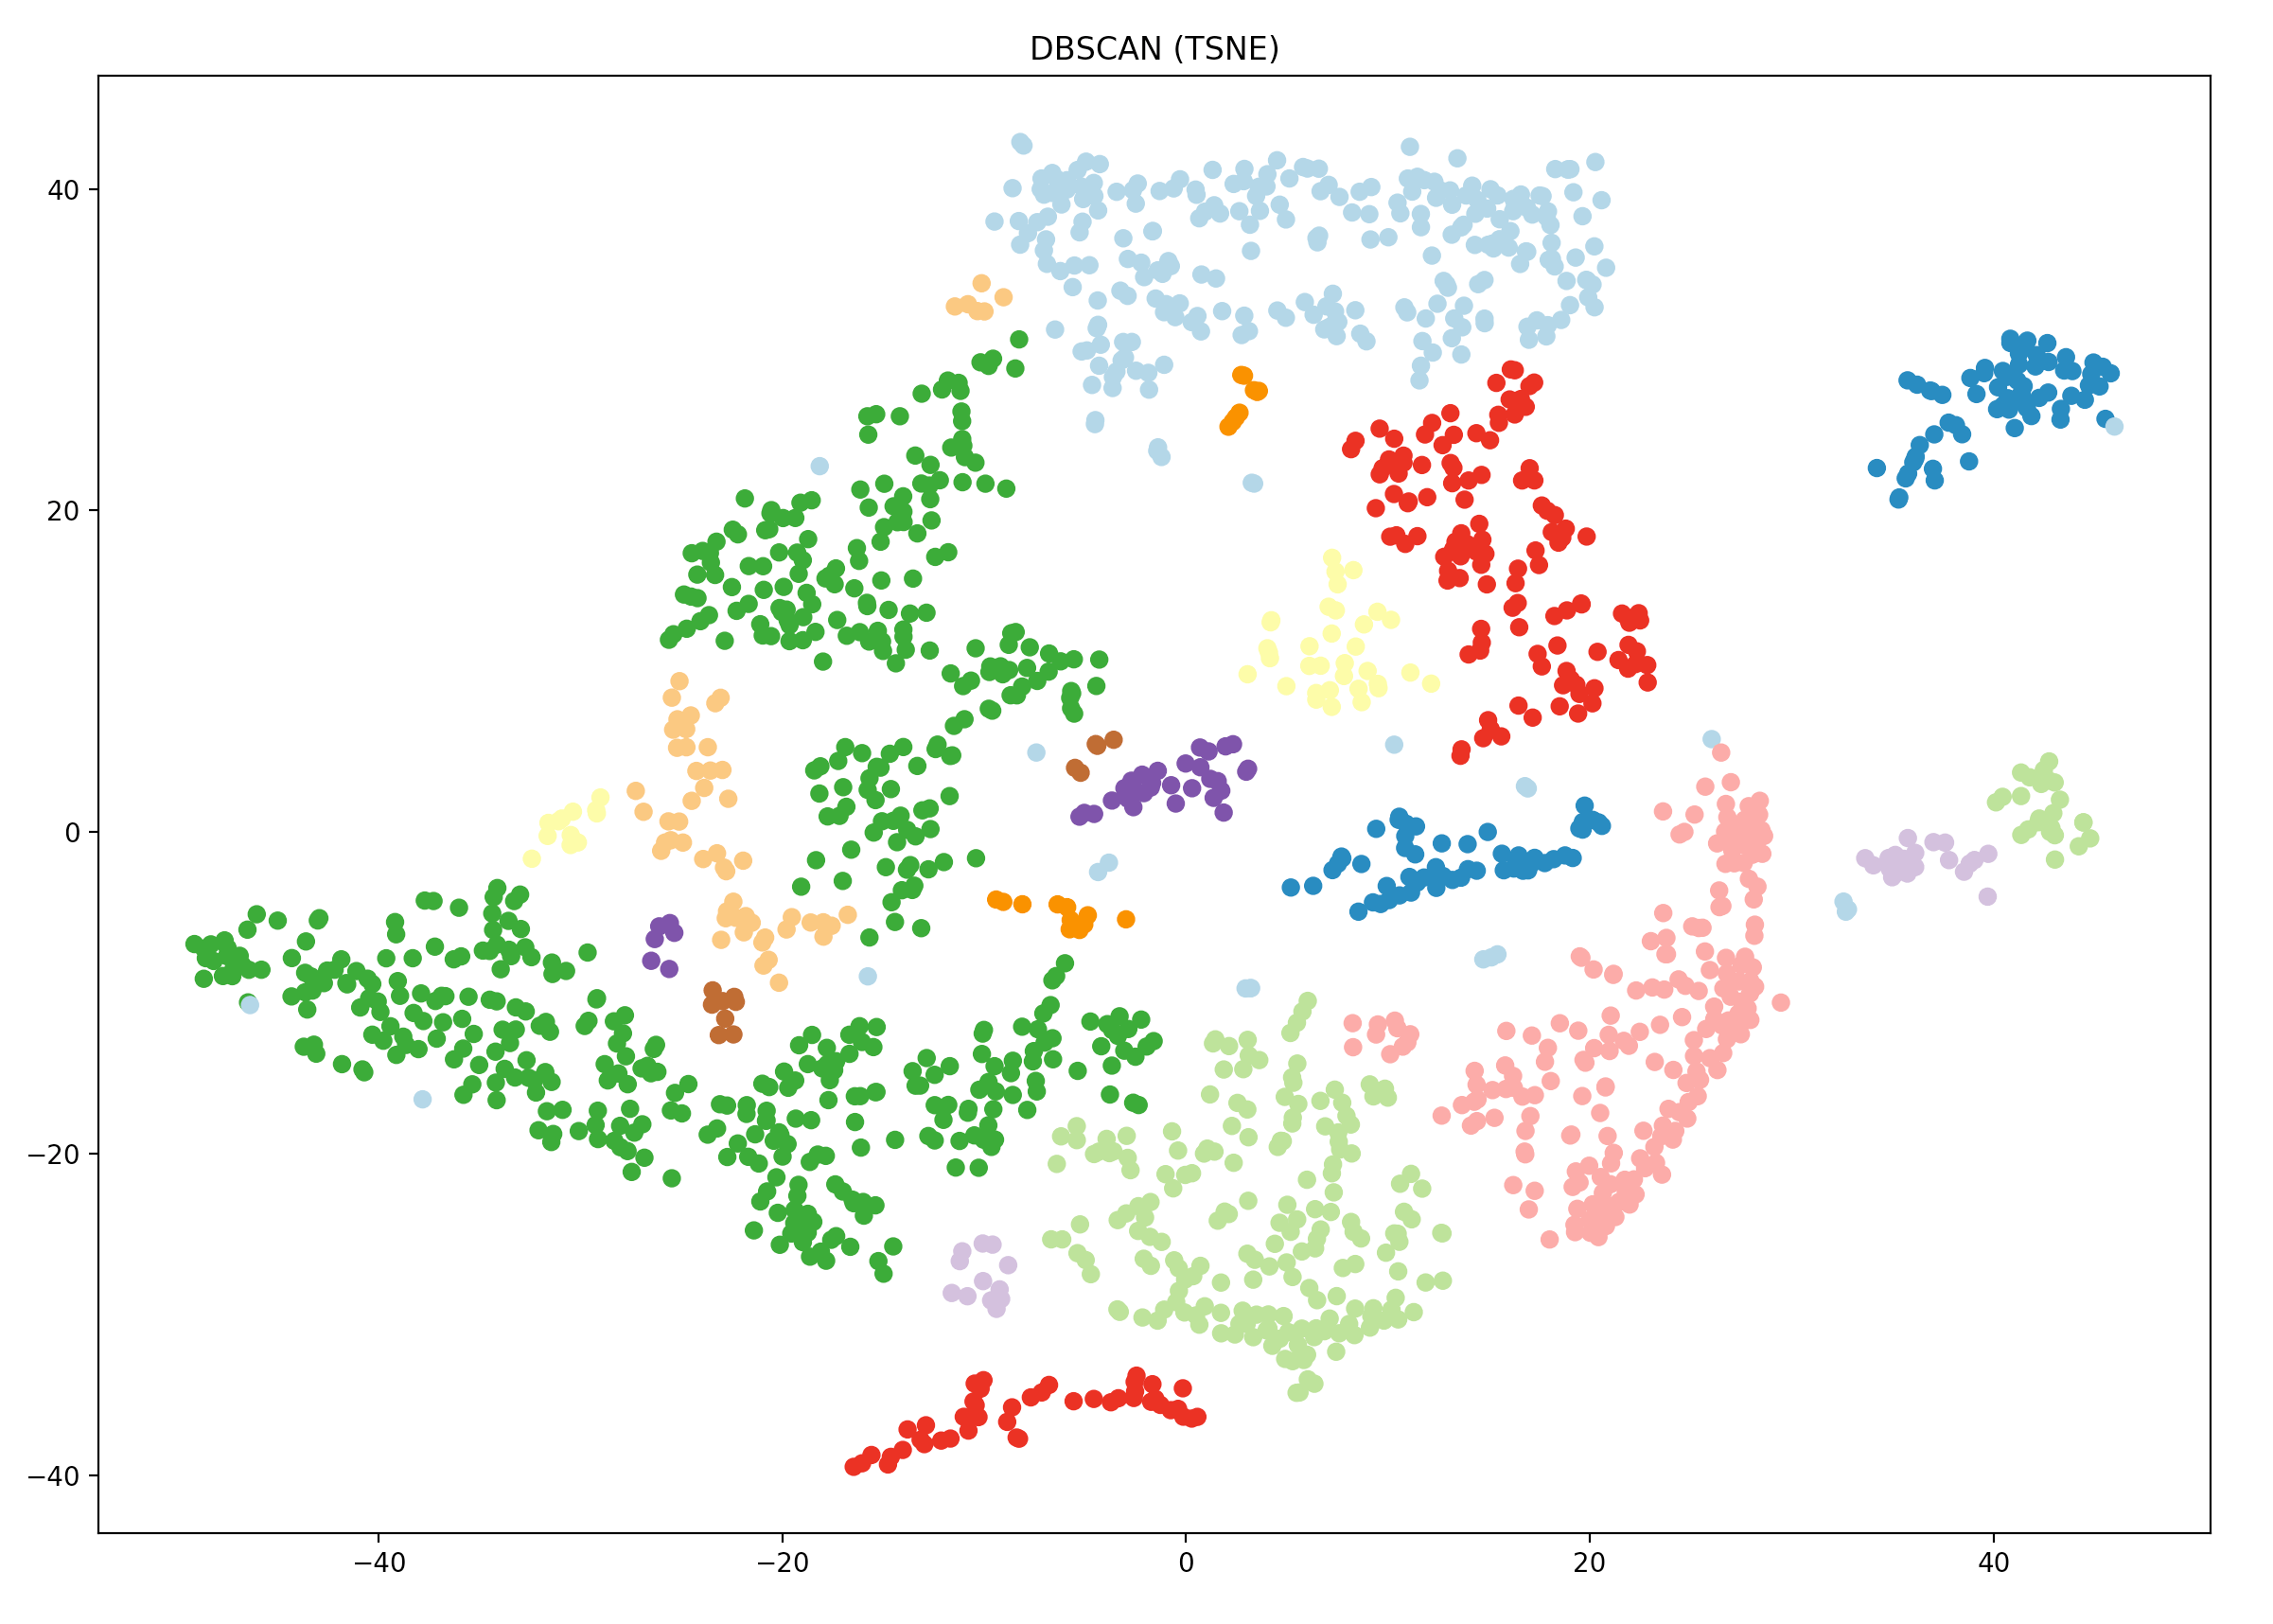
\includegraphics[width=0.9\textwidth]{./images/tsneParametersTest/learningRate/lr10-1hDBSCAN.png}
    % \caption{}
    % \label{figure:}
  \end{subfigure}
	\caption{\textbf{1h} data files, t-SNE calculated with the following parameters: perplexity=40, n\_iter=5000, \textbf{learning\_rate=10}}
	\label{figure:1hlr10TSNE}
\end{figure}

% -- 3h, lr 10 --
\begin{figure}[H]
	\centering
	
  \centering
	\begin{subfigure}{.5\textwidth}
    \centering
    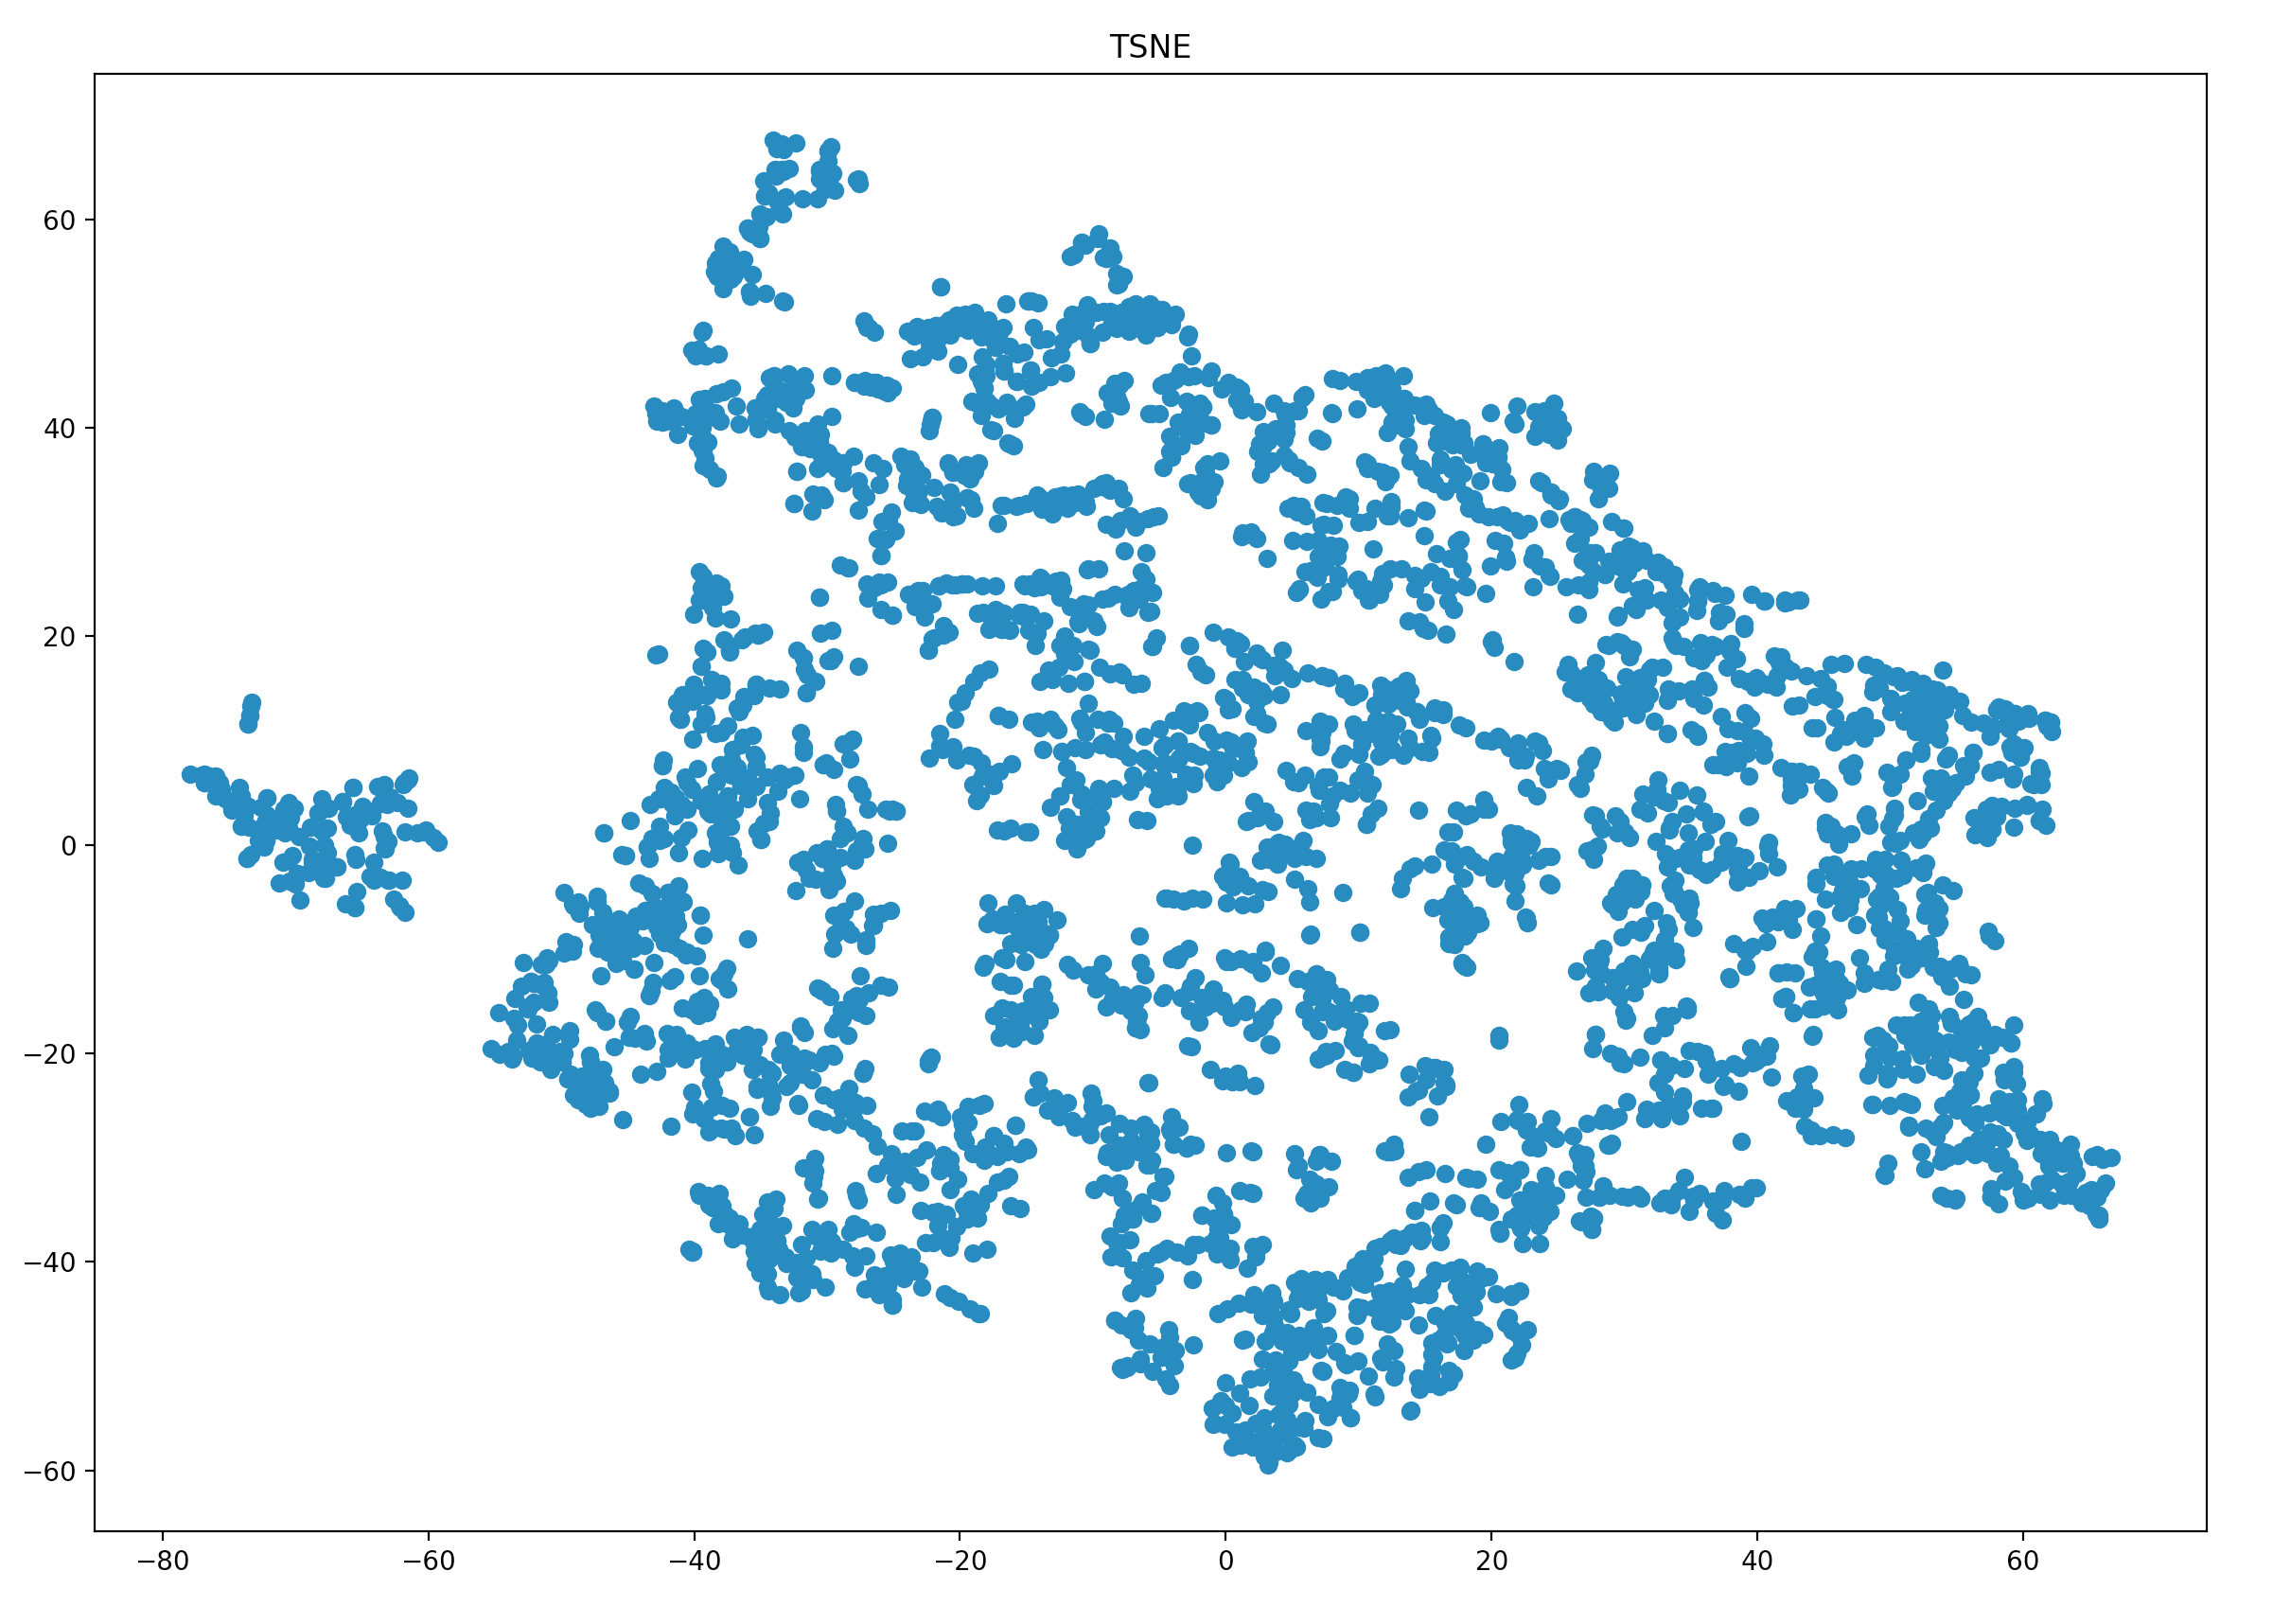
\includegraphics[width=0.9\textwidth]{./images/tsneParametersTest/learningRate/lr10-3hTSNE.png}
  % \caption{}
  % \label{figure:}
  \end{subfigure}%
  \begin{subfigure}{.5\textwidth}
    \centering
    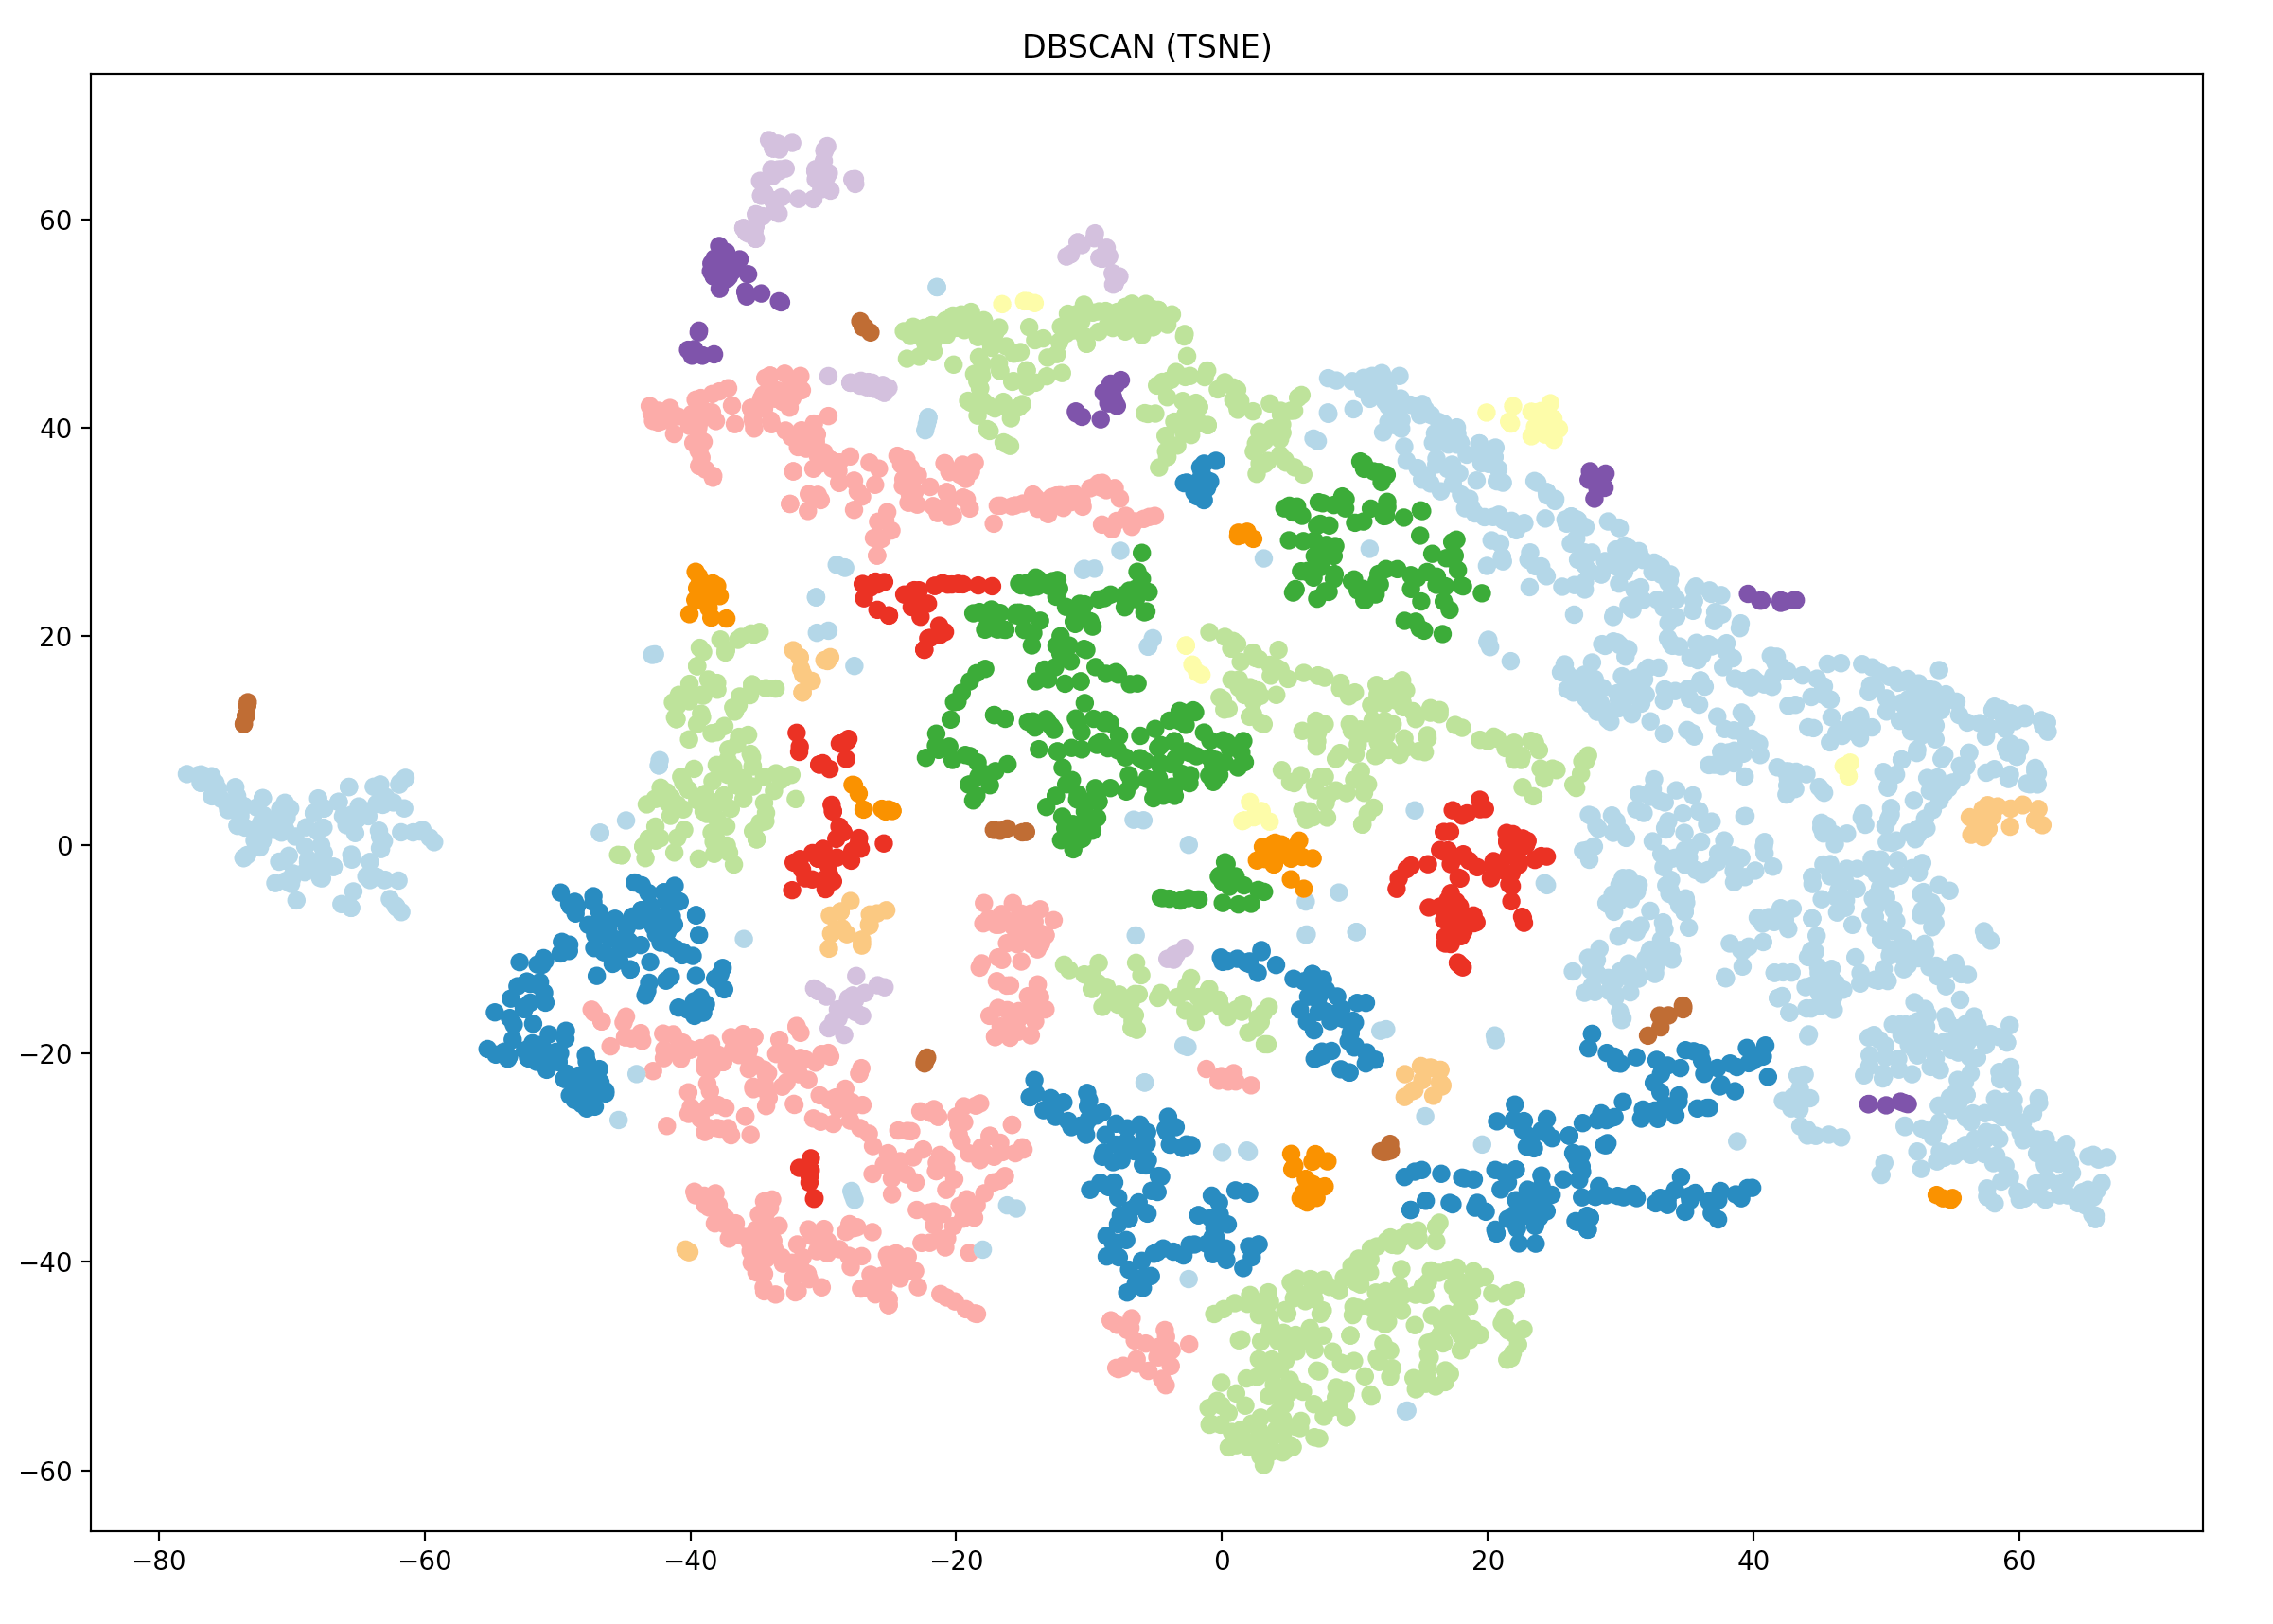
\includegraphics[width=0.9\textwidth]{./images/tsneParametersTest/learningRate/lr10-3hDBSCAN.png}
    % \caption{}
    % \label{figure:}
	\end{subfigure}
	\caption{\textbf{3h} data files, t-SNE calculated with the following parameters: perplexity=40, n\_iter=5000, \textbf{learning\_rate=10}}
  \label{figure:3hlr10TSNE}
\end{figure}

%------------------ LEARNING RATE 200: ------------------
\subsubsection{Learning Rate = 200}
% -- 1h, lr 200 --
\begin{figure}[H]
  \centering
  \begin{subfigure}{.5\textwidth}
    \centering
    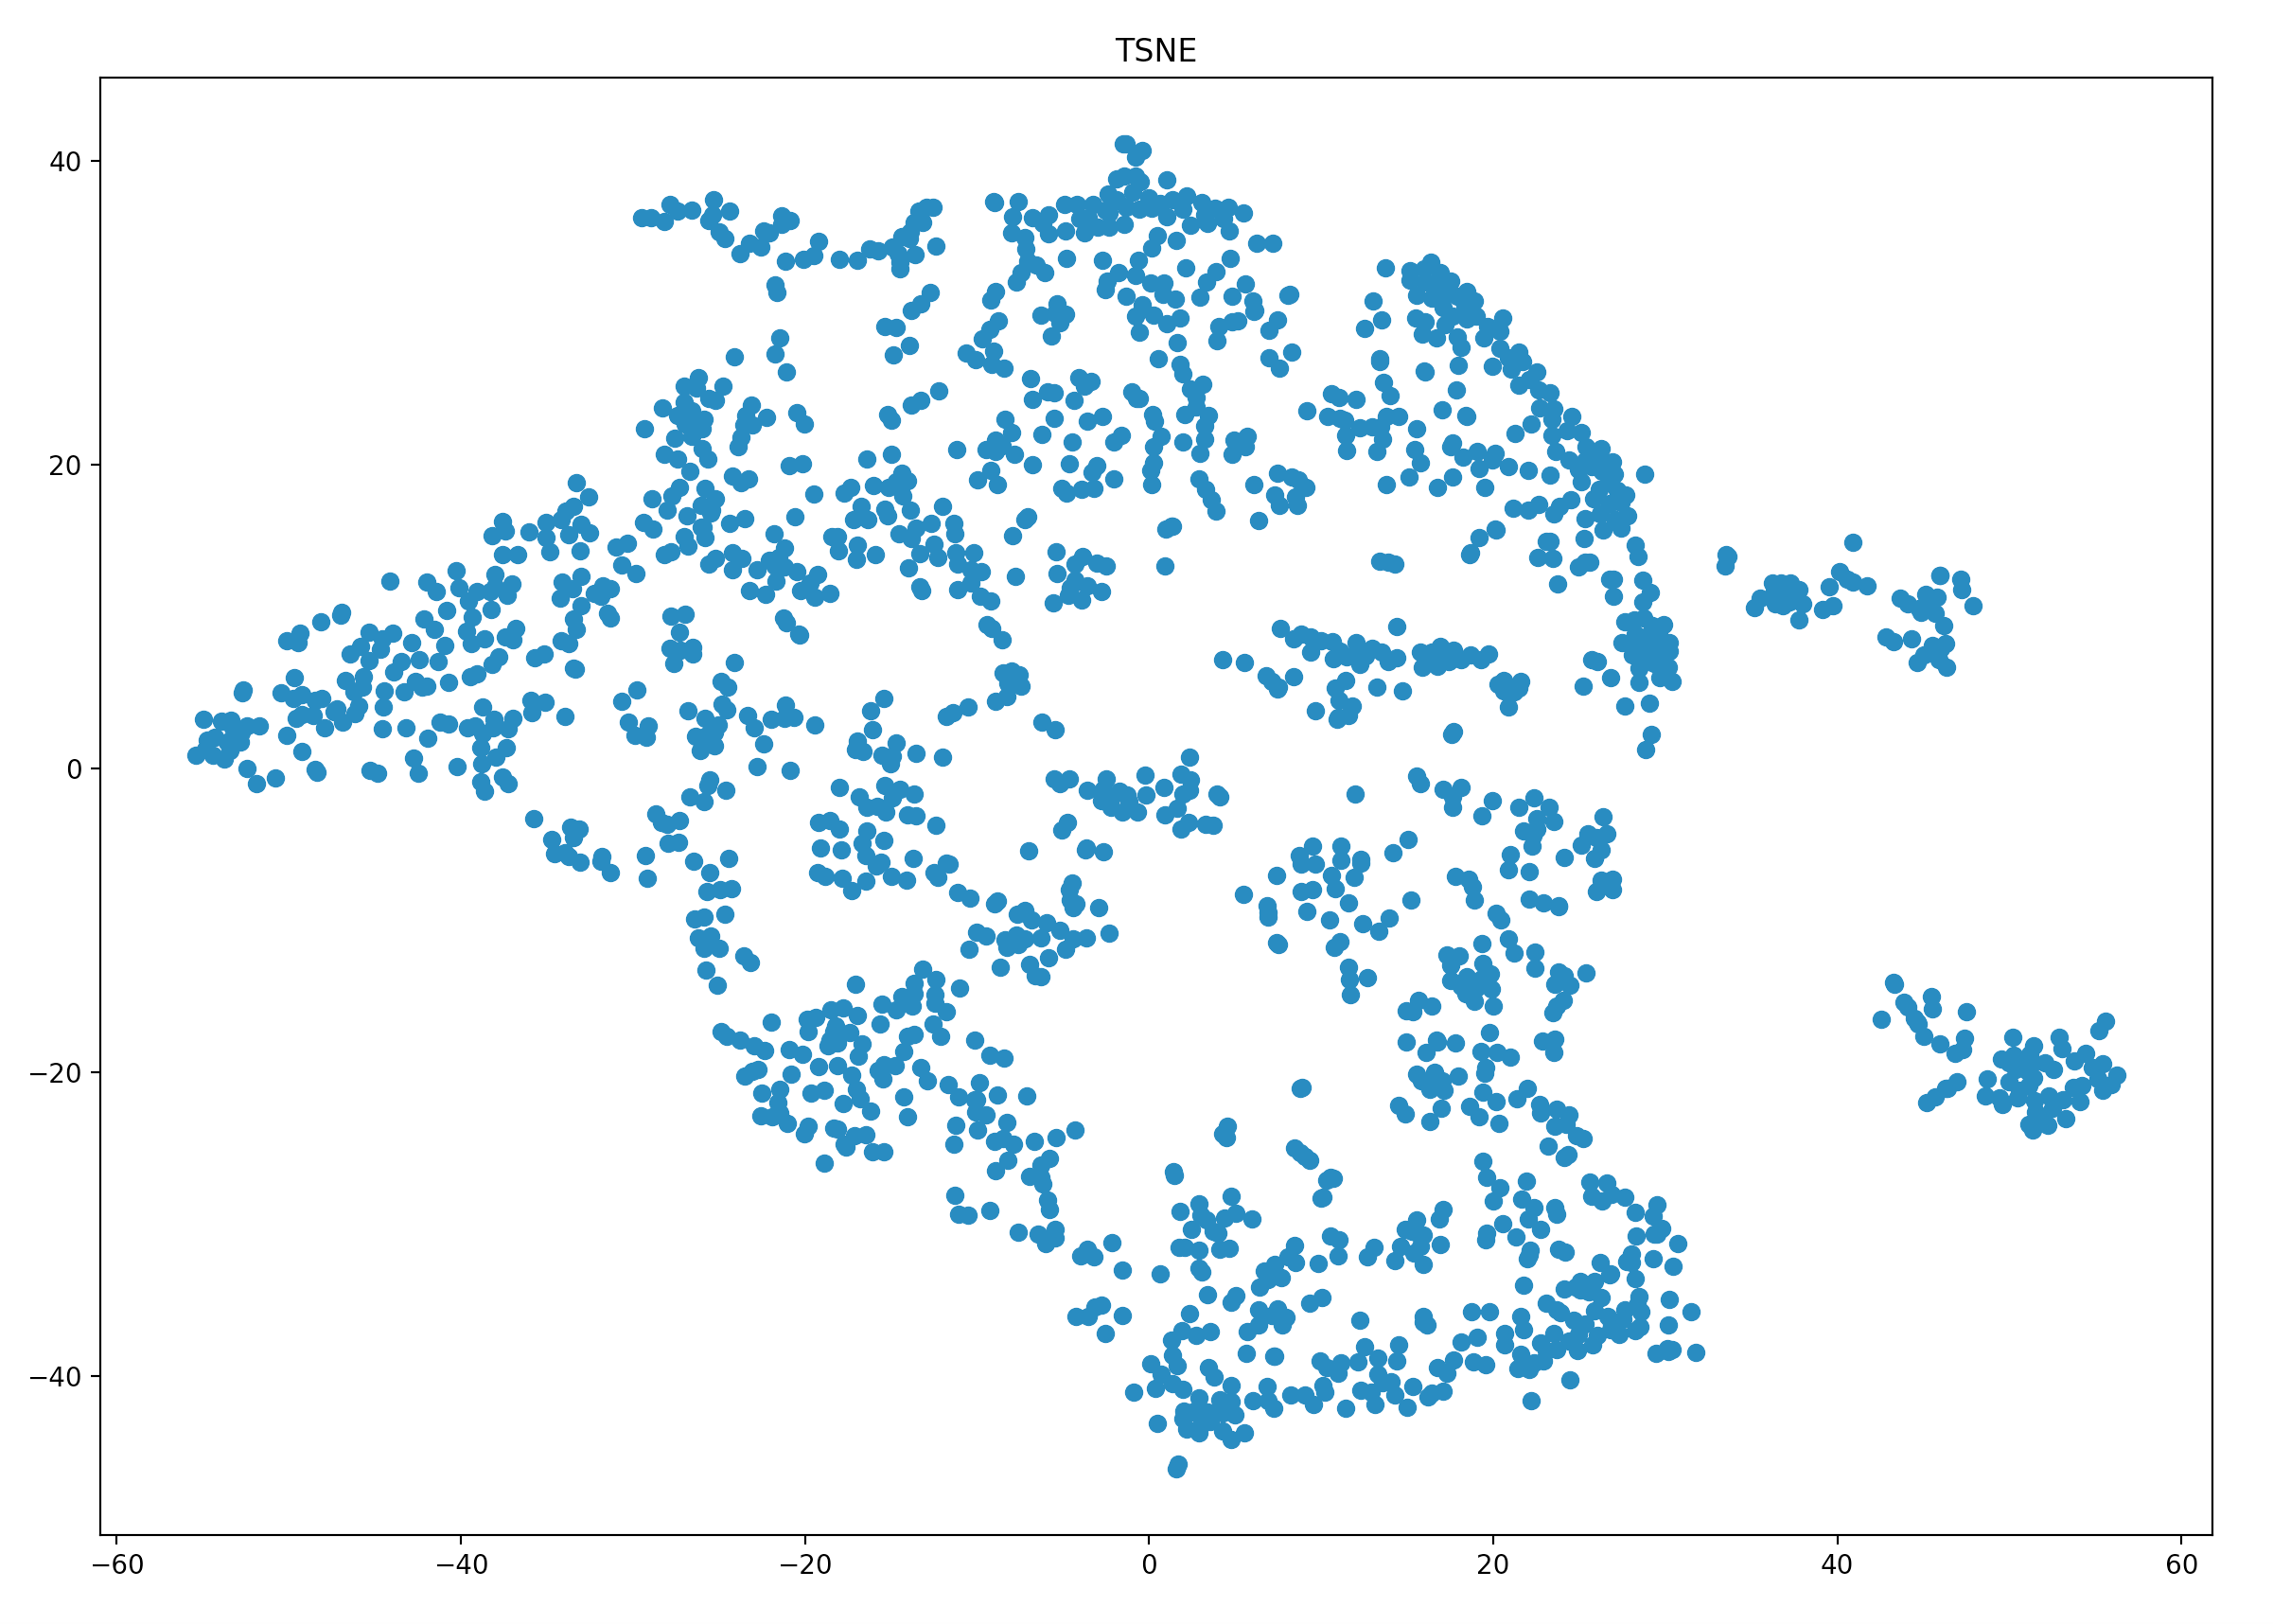
\includegraphics[width=0.9\textwidth]{./images/tsneParametersTest/learningRate/lr200-1hTSNE.png}
  % \caption{}
  % \label{figure:}
  \end{subfigure}%
  \begin{subfigure}{.5\textwidth}
    \centering
    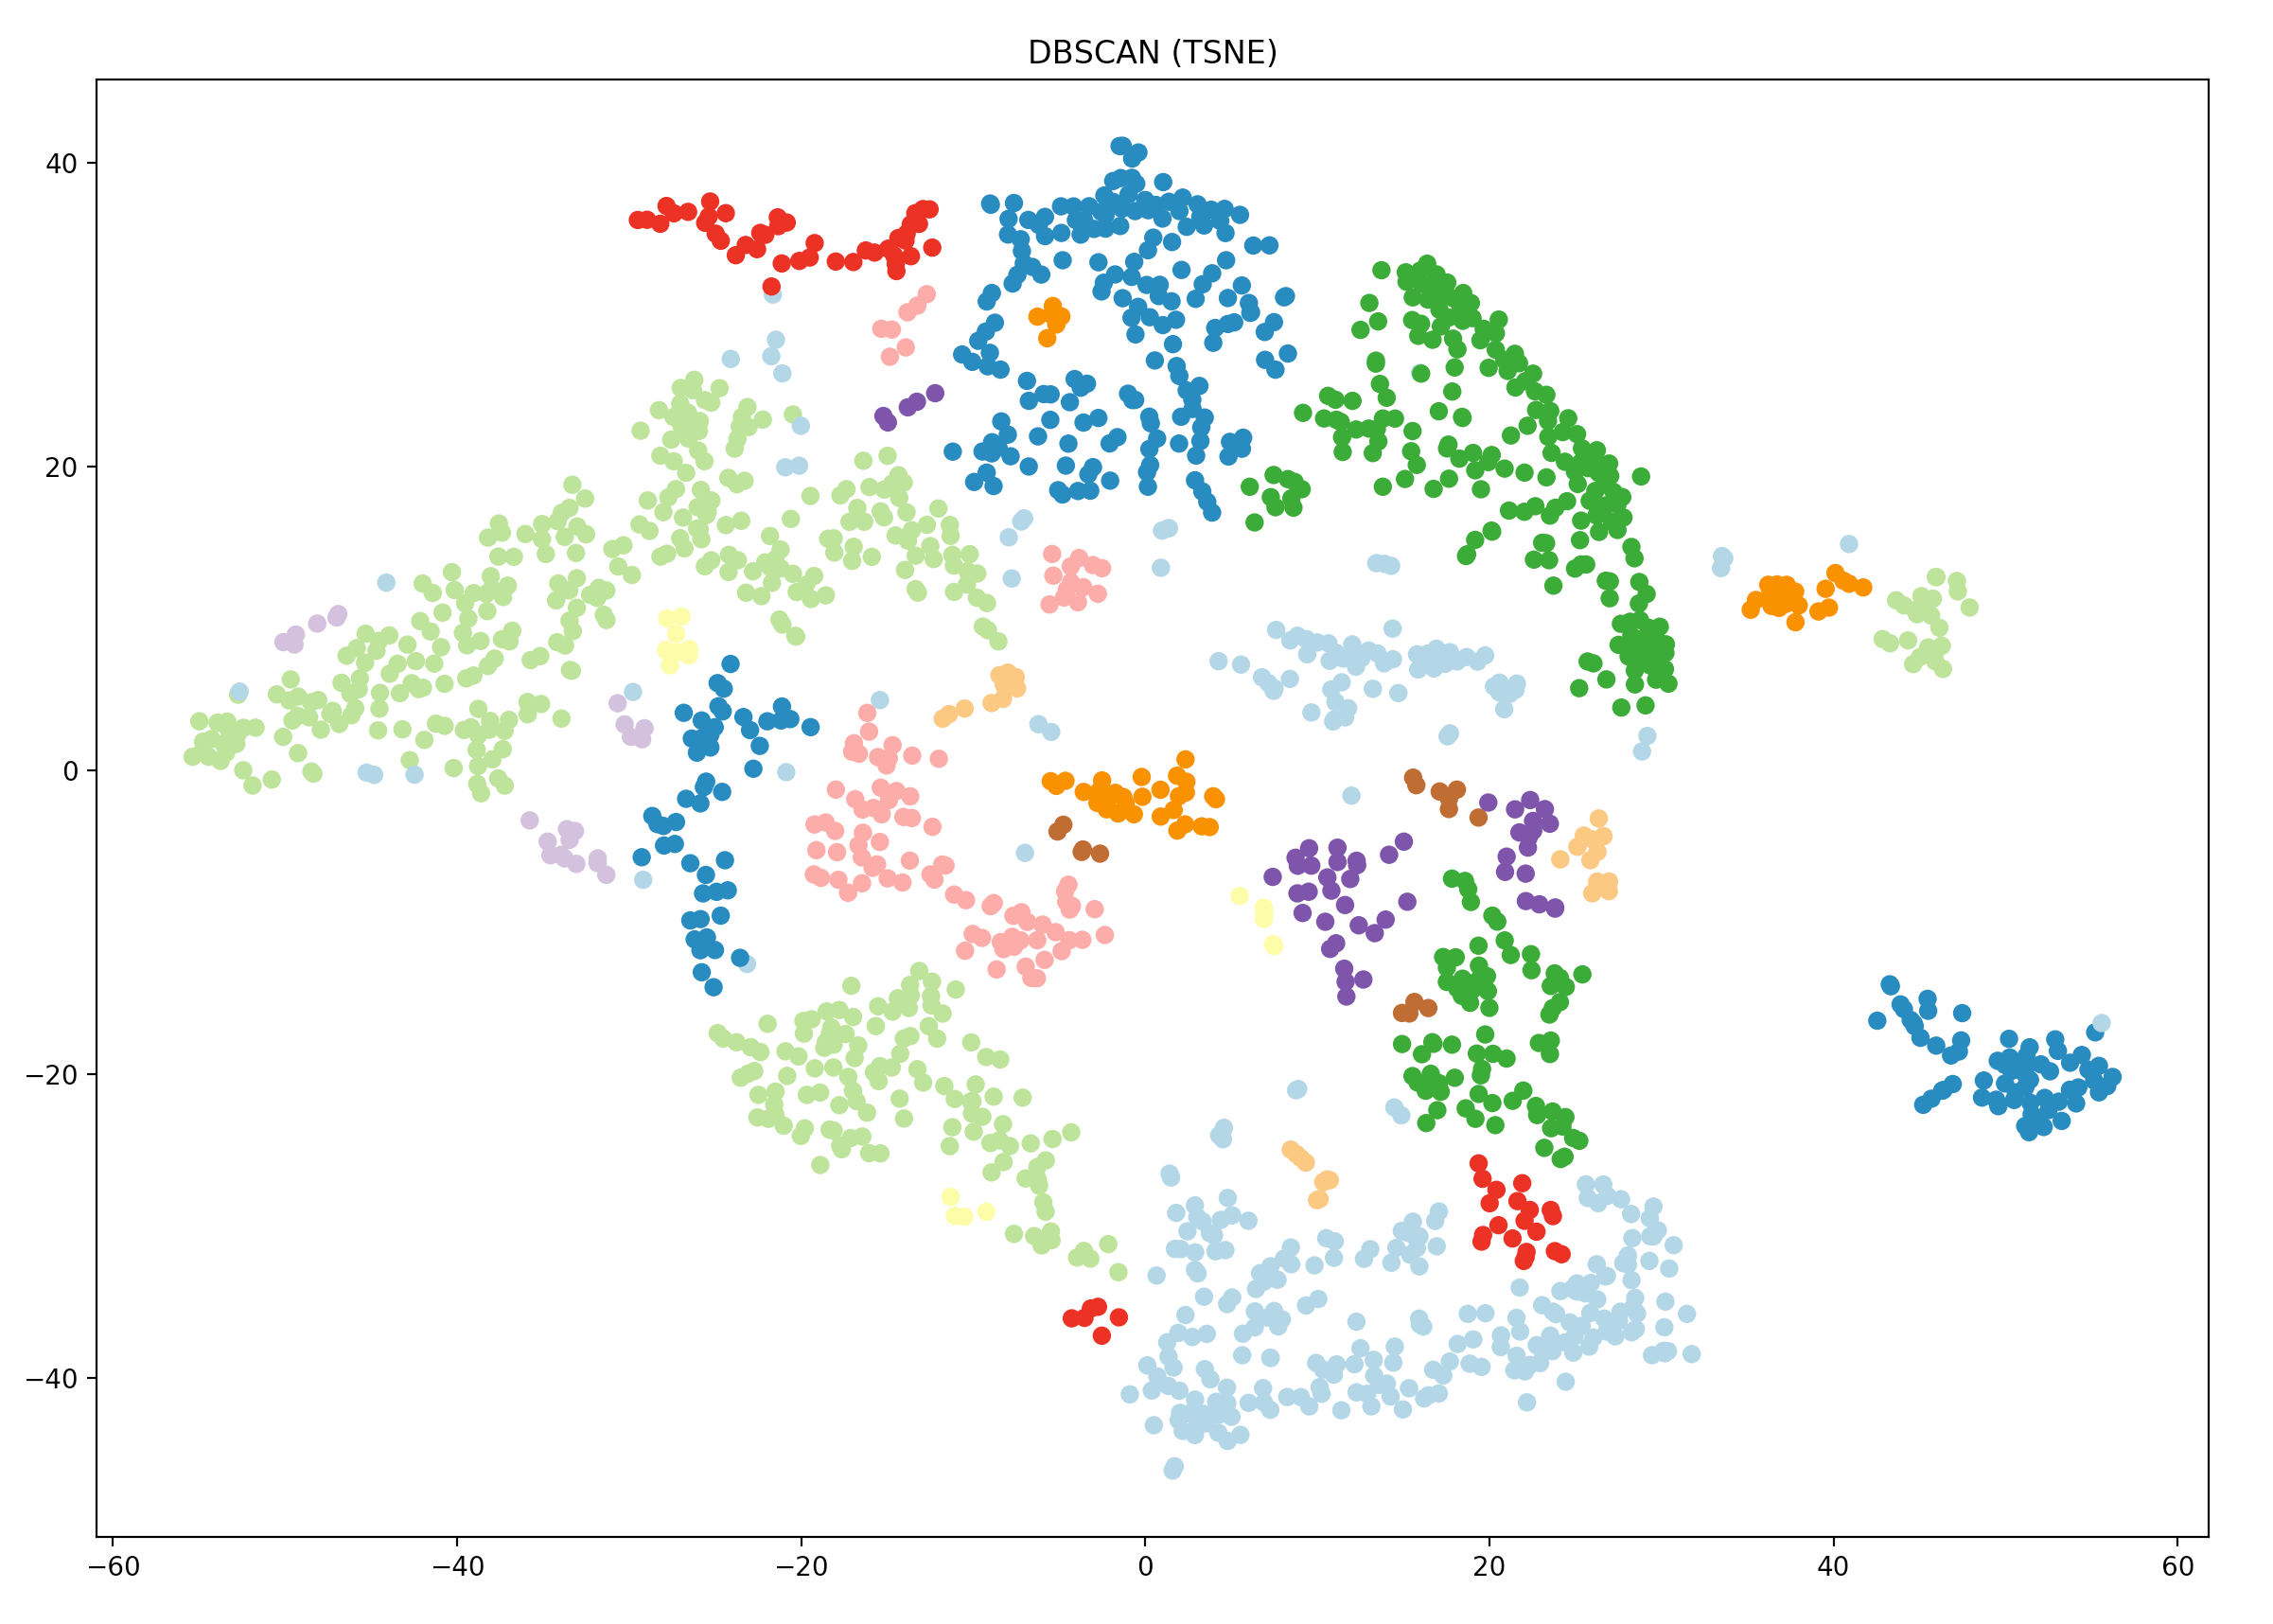
\includegraphics[width=0.9\textwidth]{./images/tsneParametersTest/learningRate/lr200-1hDBSCAN.png}
    % \caption{}
    % \label{figure:}
  \end{subfigure}
	\caption{\textbf{1h} data files, t-SNE calculated with the following parameters: perplexity=40, n\_iter=5000, \textbf{learning\_rate=200}}
	\label{figure:1hlr200TSNE}
\end{figure}

% -- 3h, lr 200 --
\begin{figure}[H]
	\centering
	
  \centering
	\begin{subfigure}{.5\textwidth}
    \centering
    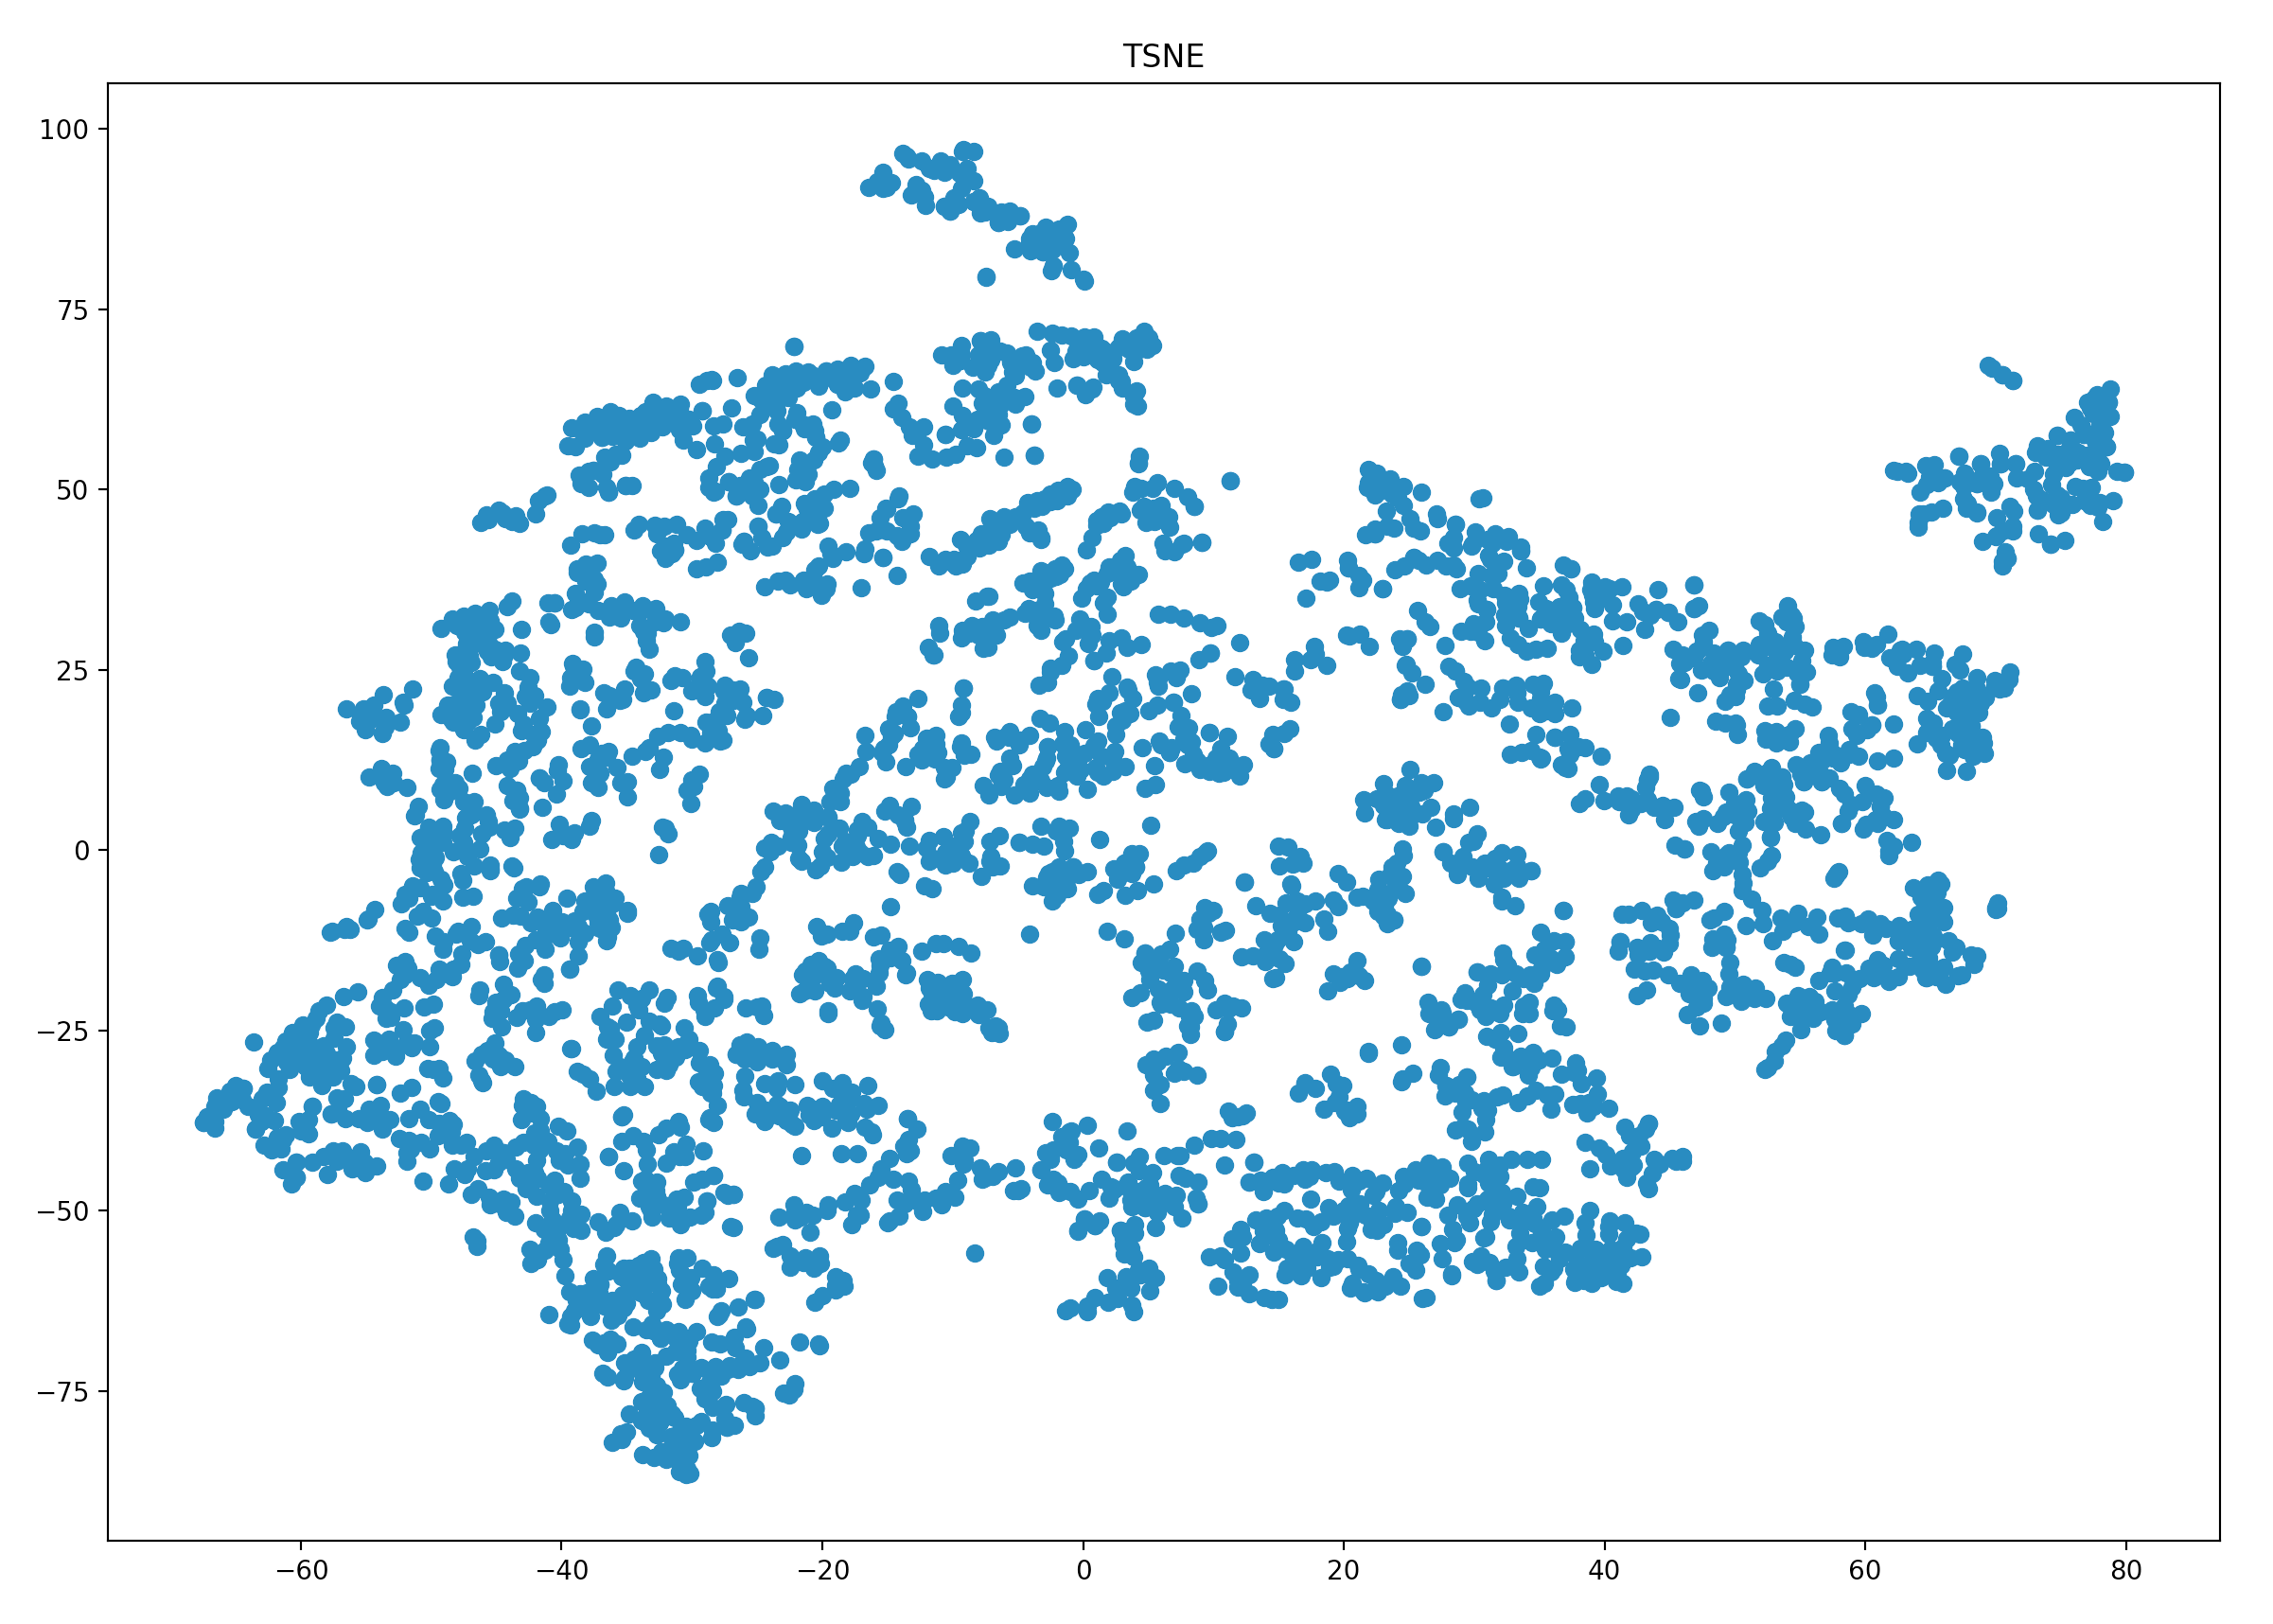
\includegraphics[width=0.9\textwidth]{./images/tsneParametersTest/learningRate/lr200-3hTSNE.png}
  % \caption{}
  % \label{figure:}
  \end{subfigure}%
  \begin{subfigure}{.5\textwidth}
    \centering
    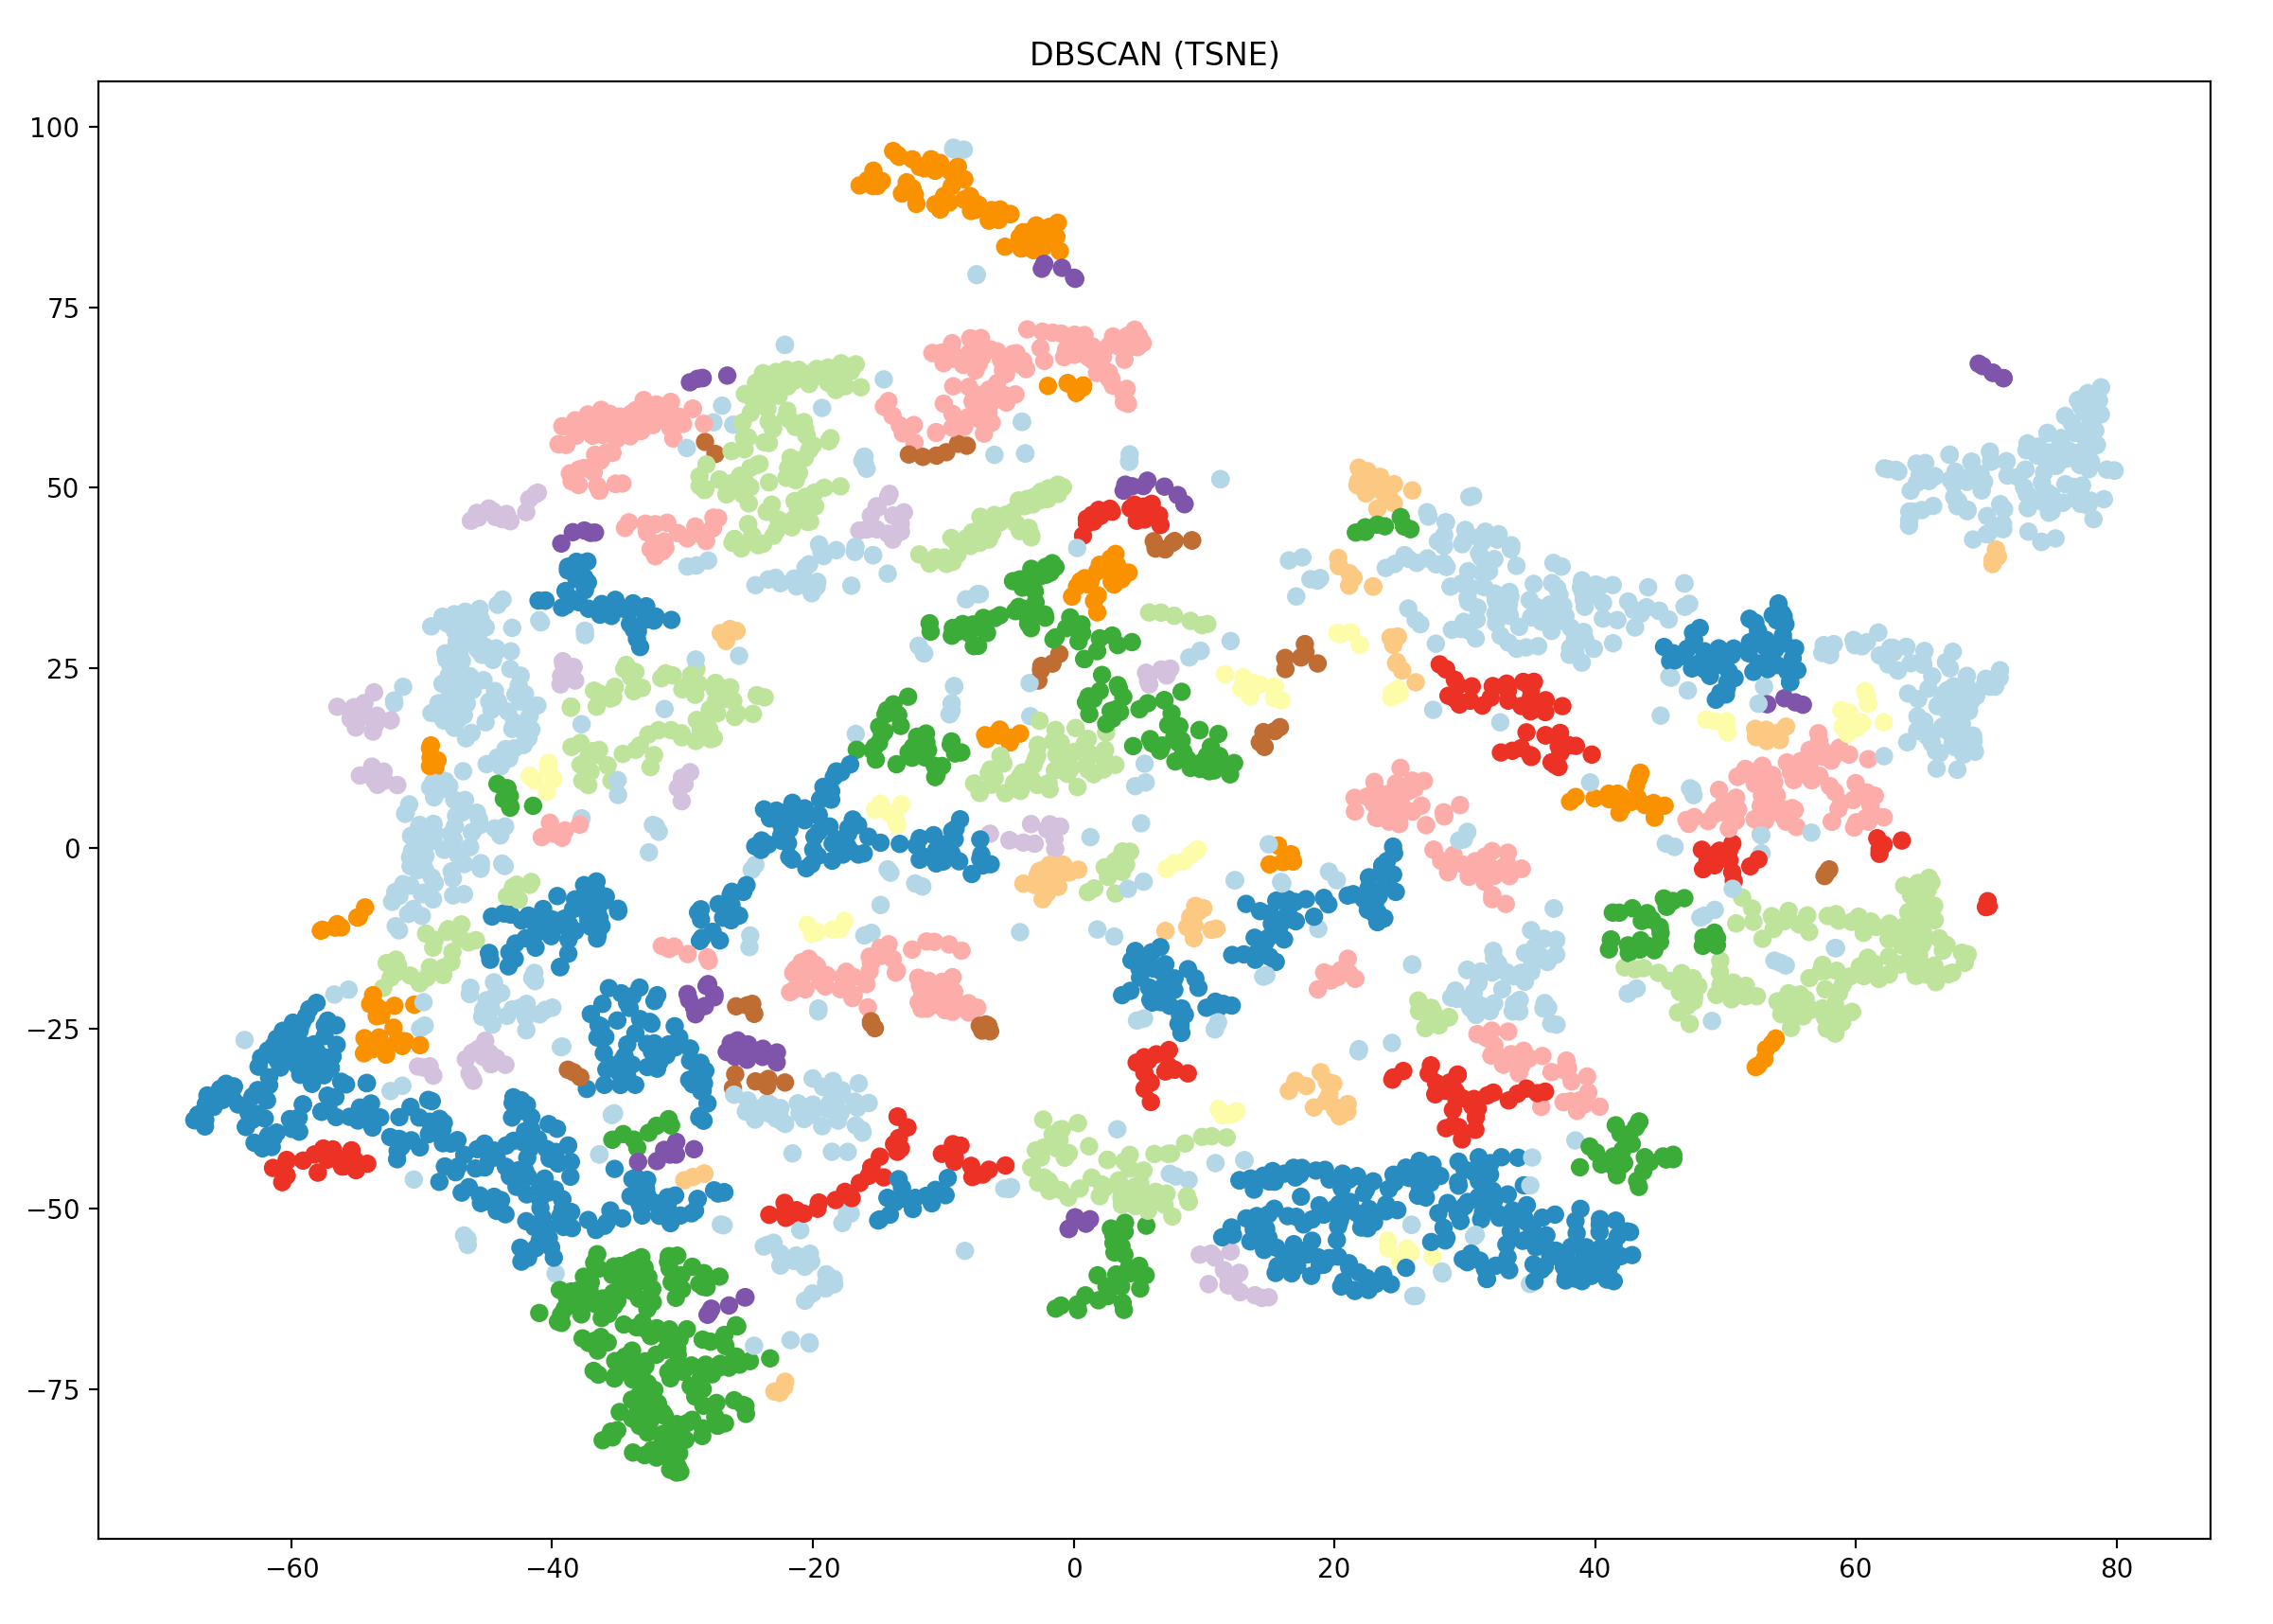
\includegraphics[width=0.9\textwidth]{./images/tsneParametersTest/learningRate/lr200-3hDBSCAN.png}
    % \caption{}
    % \label{figure:}
	\end{subfigure}
	\caption{\textbf{3h} data files, t-SNE calculated with the following parameters: perplexity=40, n\_iter=5000, \textbf{learning\_rate=200}}
  \label{figure:3hlr200TSNE}
\end{figure}


%------------------ LEARNING RATE 400: ------------------
\subsubsection{Learning Rate = 400}
% -- 1h, lr 400 --
\begin{figure}[H]
  \centering
  \begin{subfigure}{.5\textwidth}
    \centering
    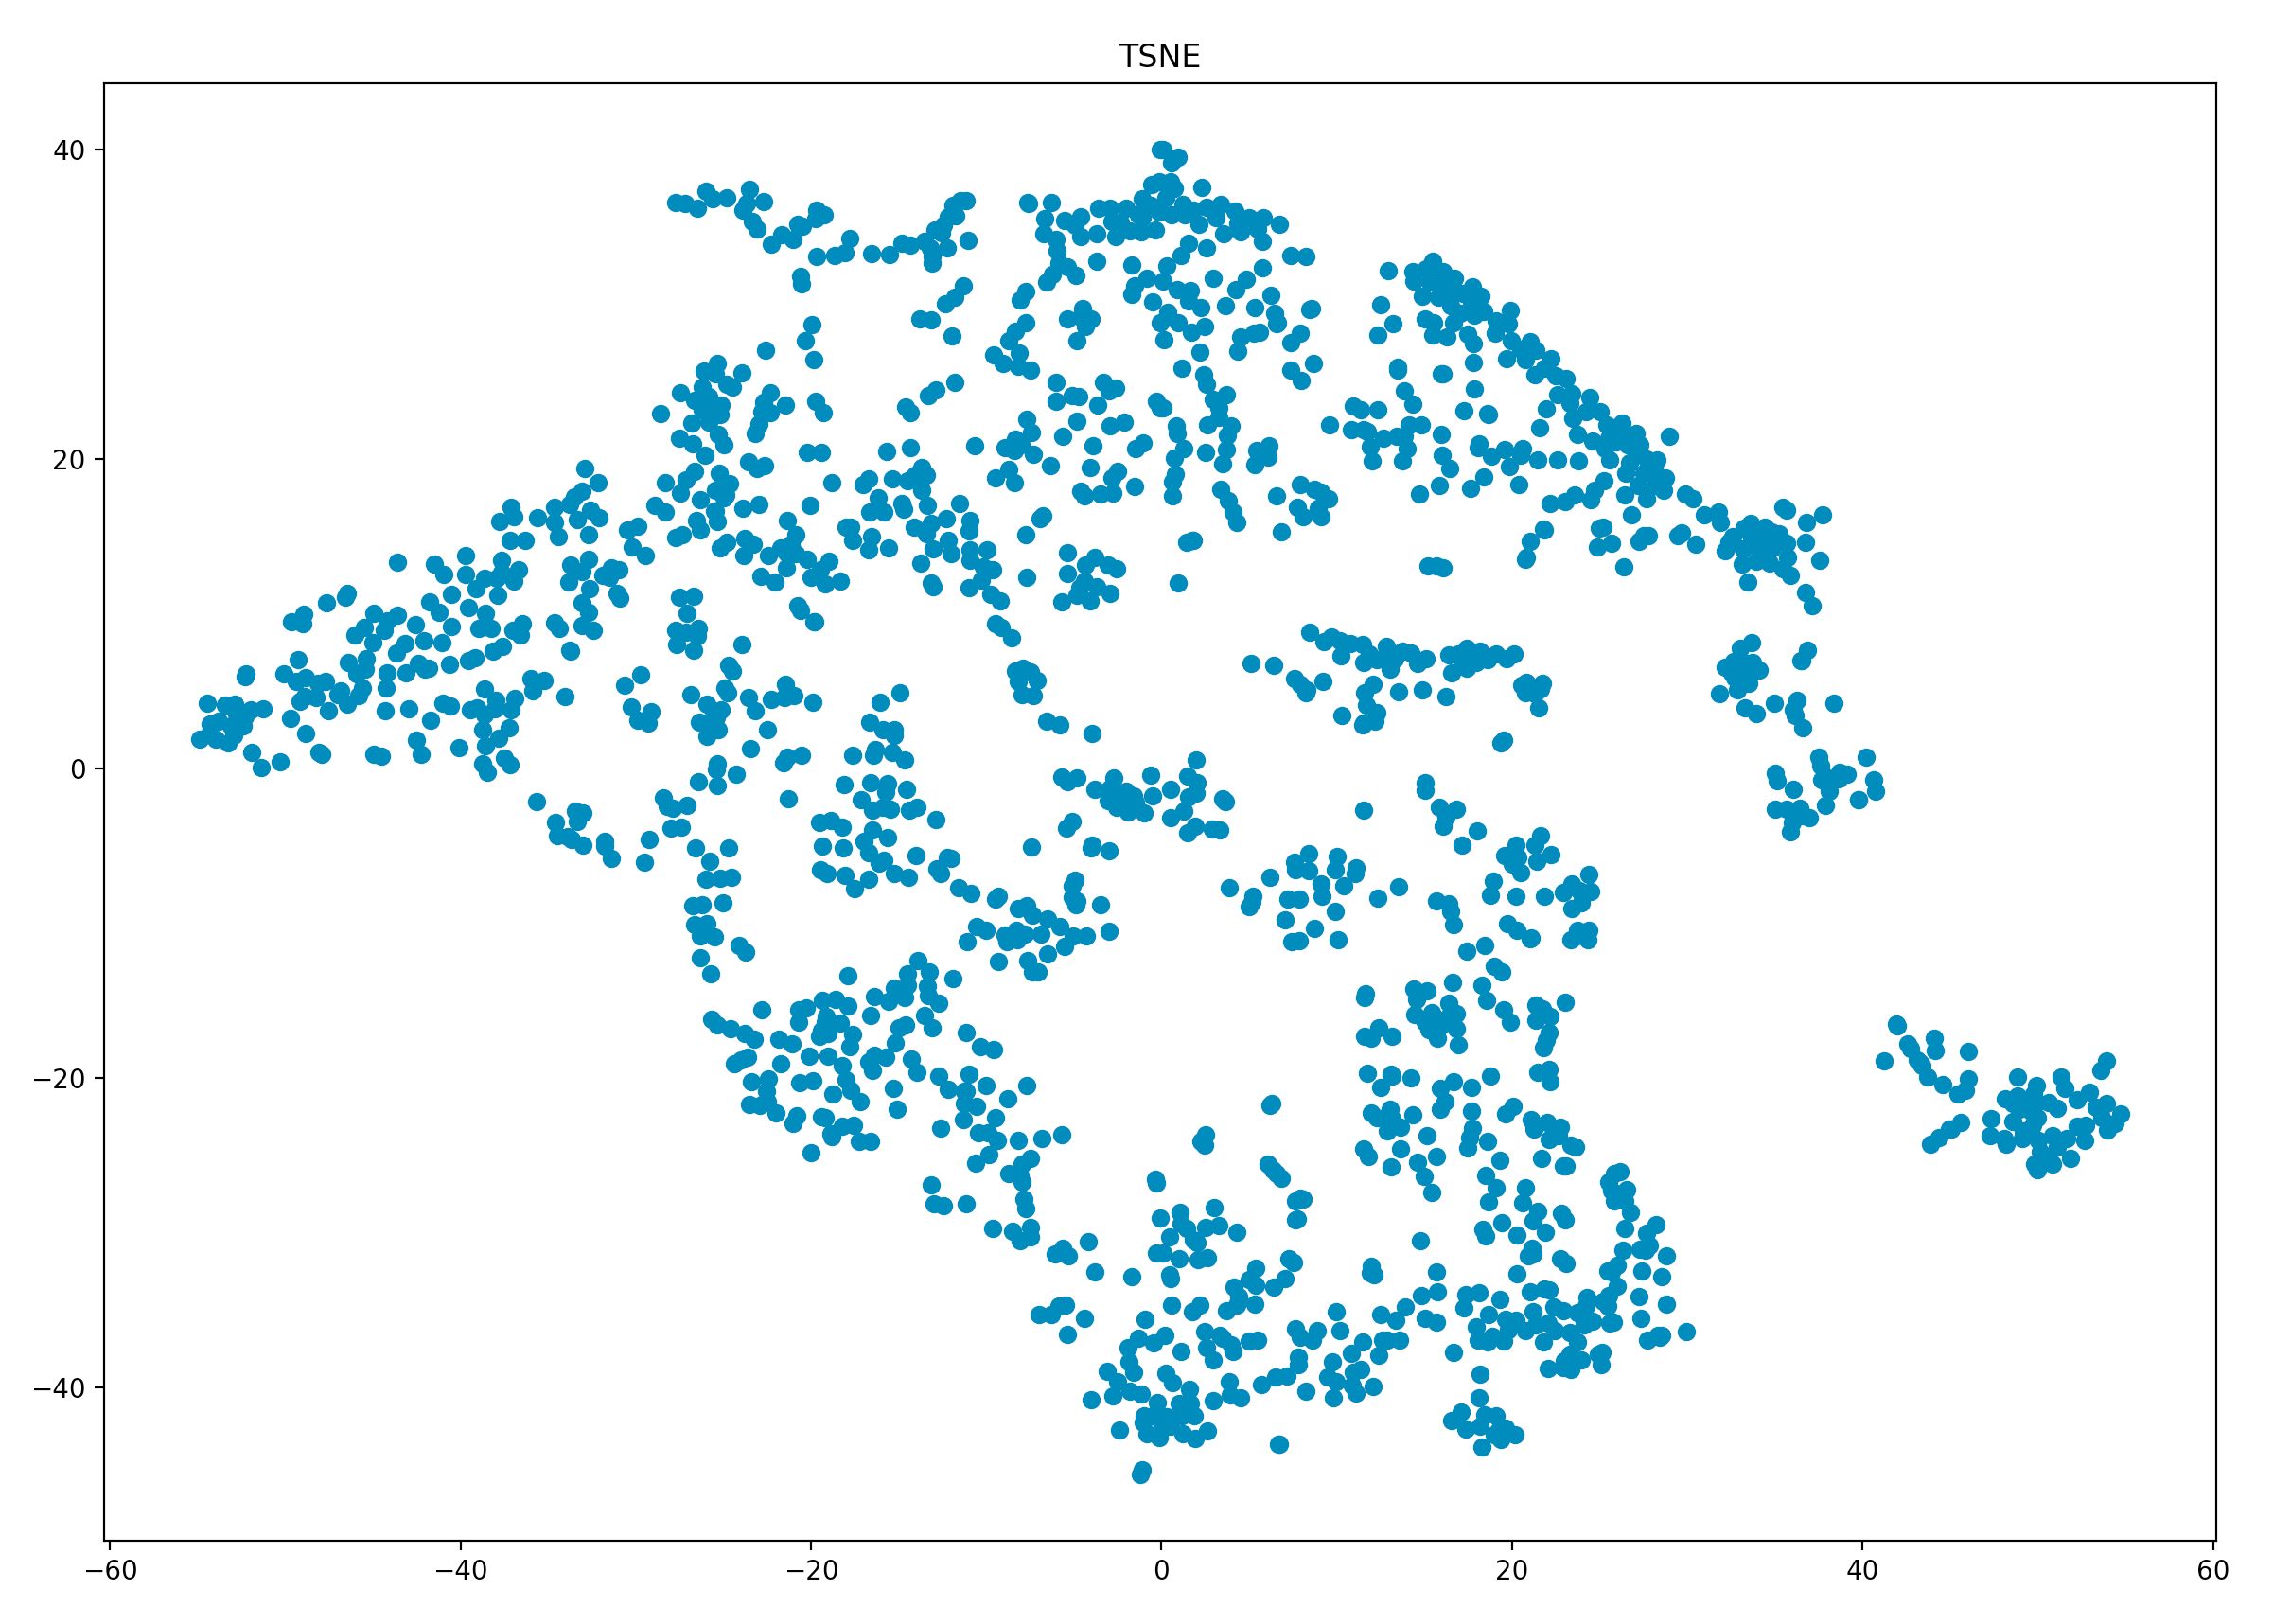
\includegraphics[width=0.9\textwidth]{./images/tsneParametersTest/learningRate/lr400-1hTSNE.png}
  % \caption{}
  % \label{figure:}
  \end{subfigure}%
  \begin{subfigure}{.5\textwidth}
    \centering
    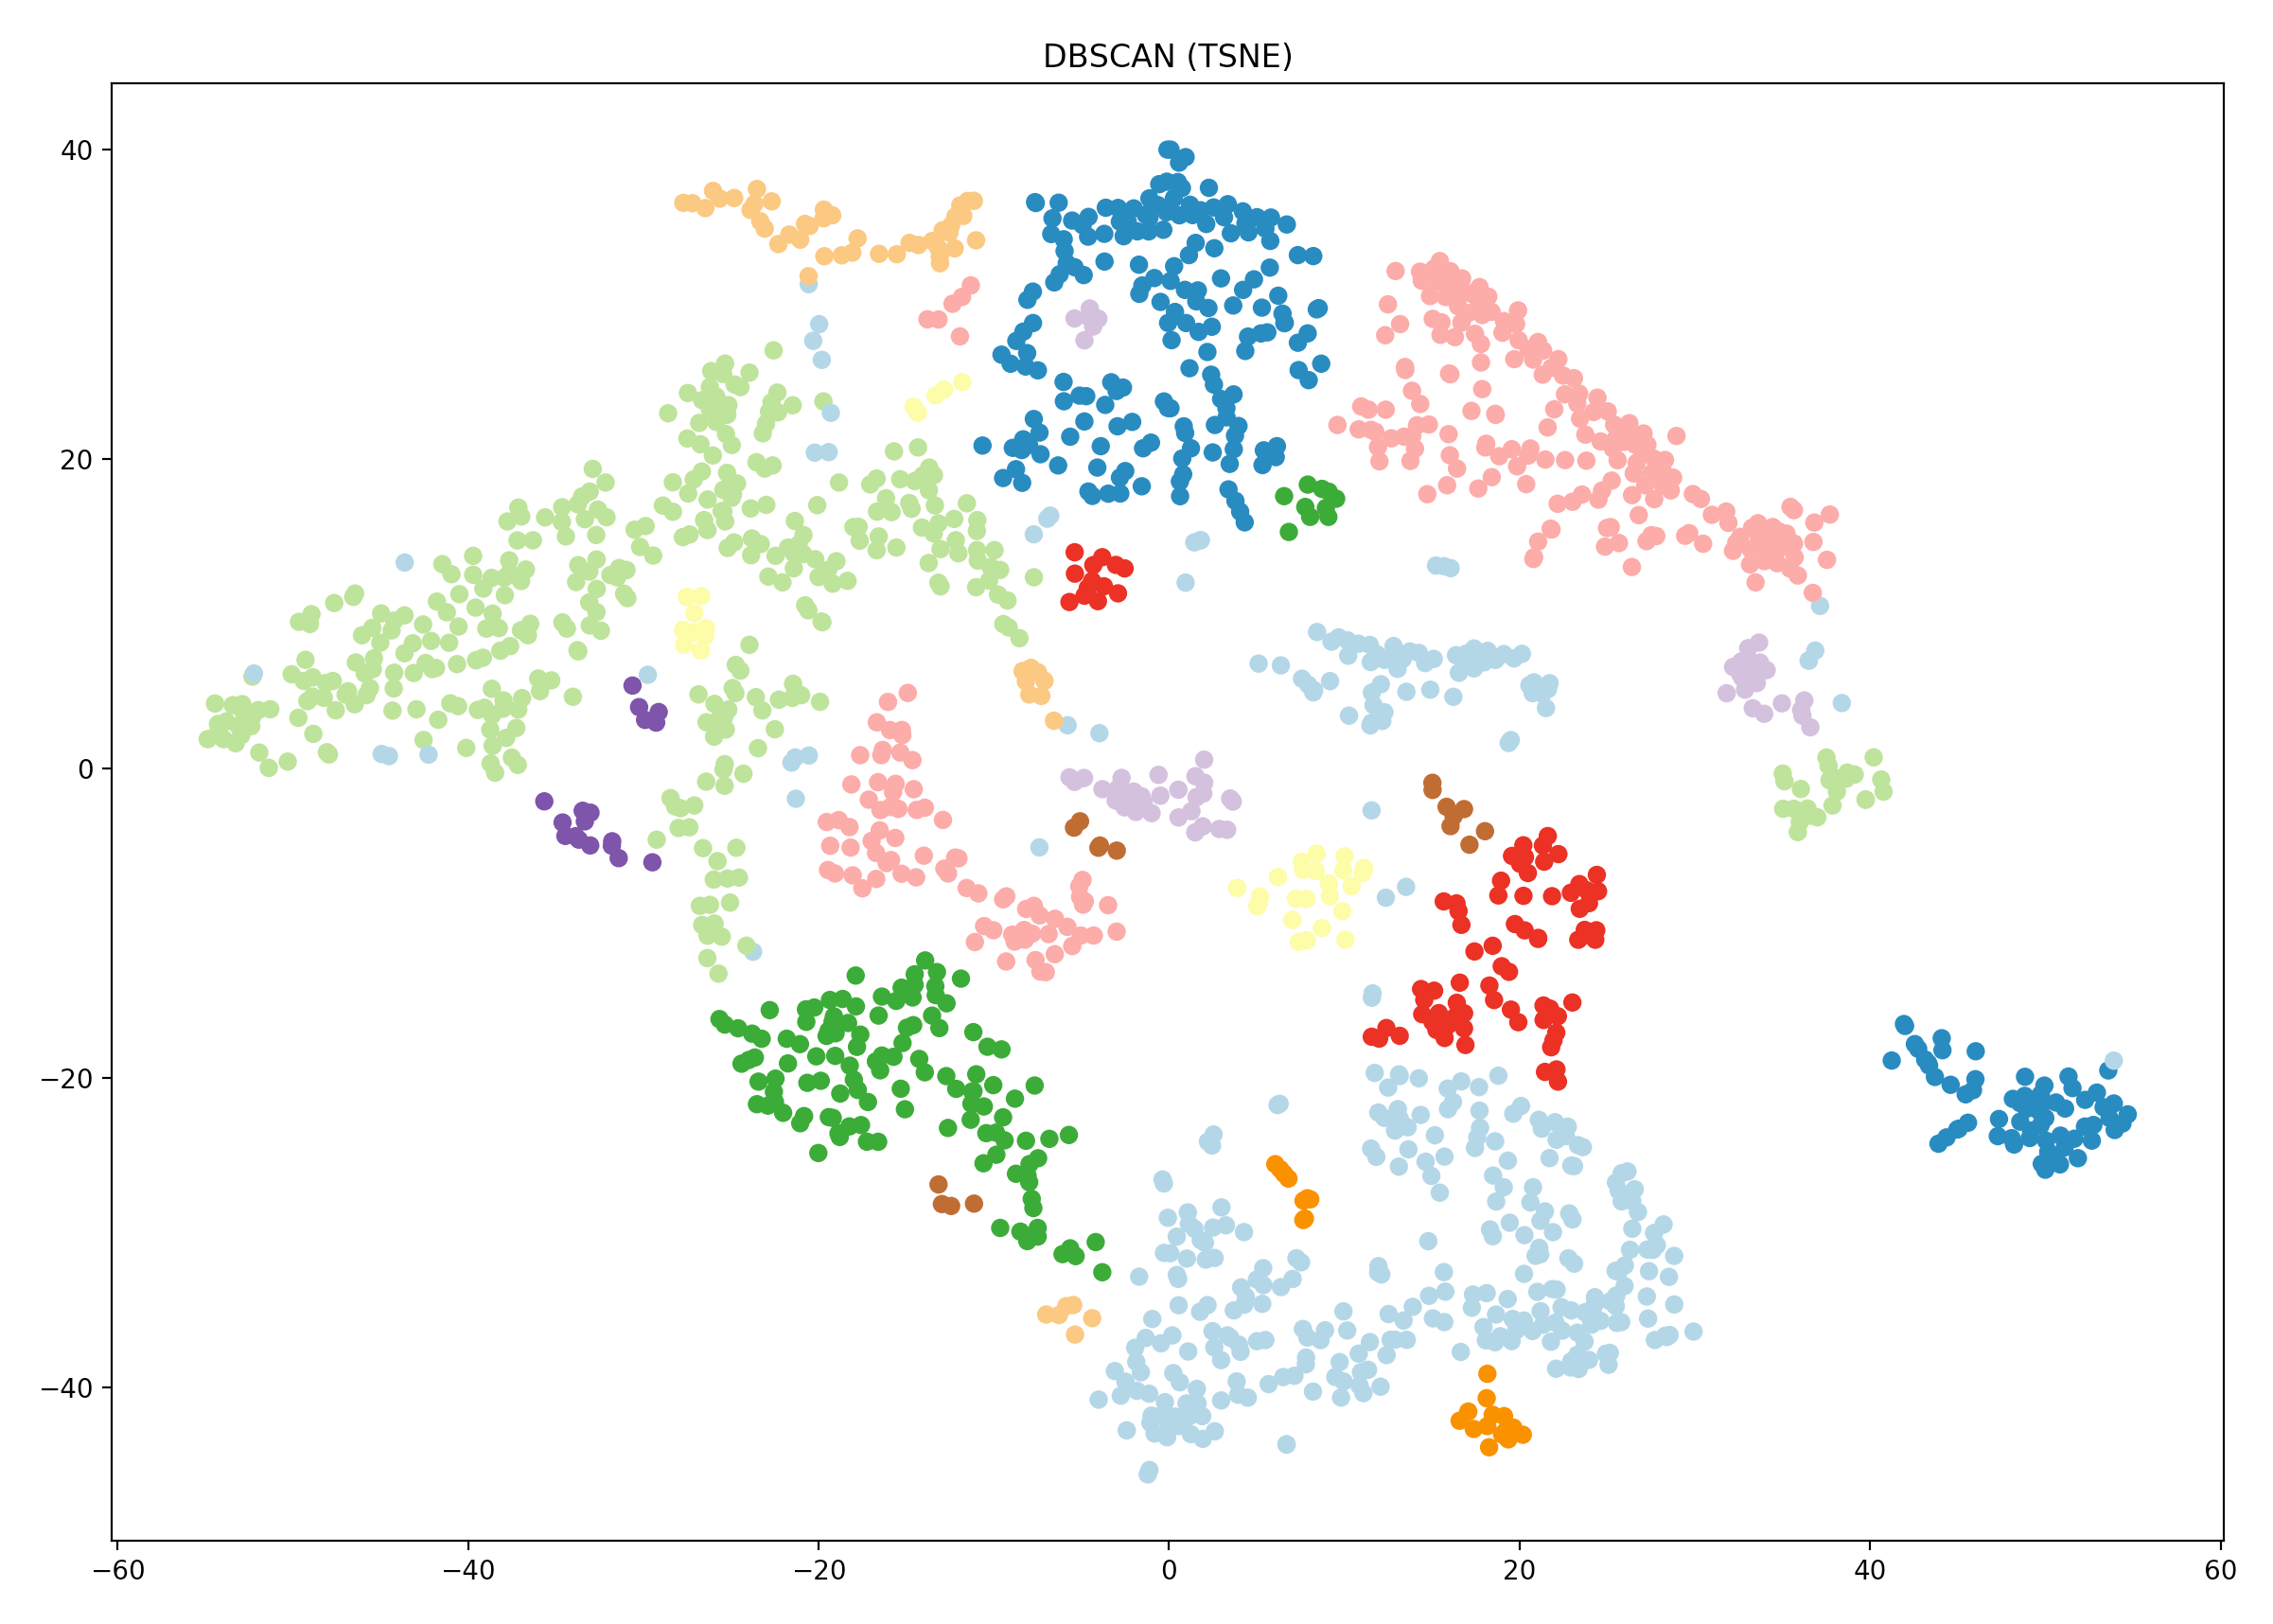
\includegraphics[width=0.9\textwidth]{./images/tsneParametersTest/learningRate/lr400-1hDBSCAN.png}
    % \caption{}
    % \label{figure:}
  \end{subfigure}
	\caption{\textbf{1h} data files, t-SNE calculated with the following parameters: perplexity=40, n\_iter=5000, \textbf{learning\_rate=400}}
	\label{figure:1hlr400TSNE}
\end{figure}

% -- 3h, lr 400 --
\begin{figure}[H]
	\centering
	
  \centering
	\begin{subfigure}{.5\textwidth}
    \centering
    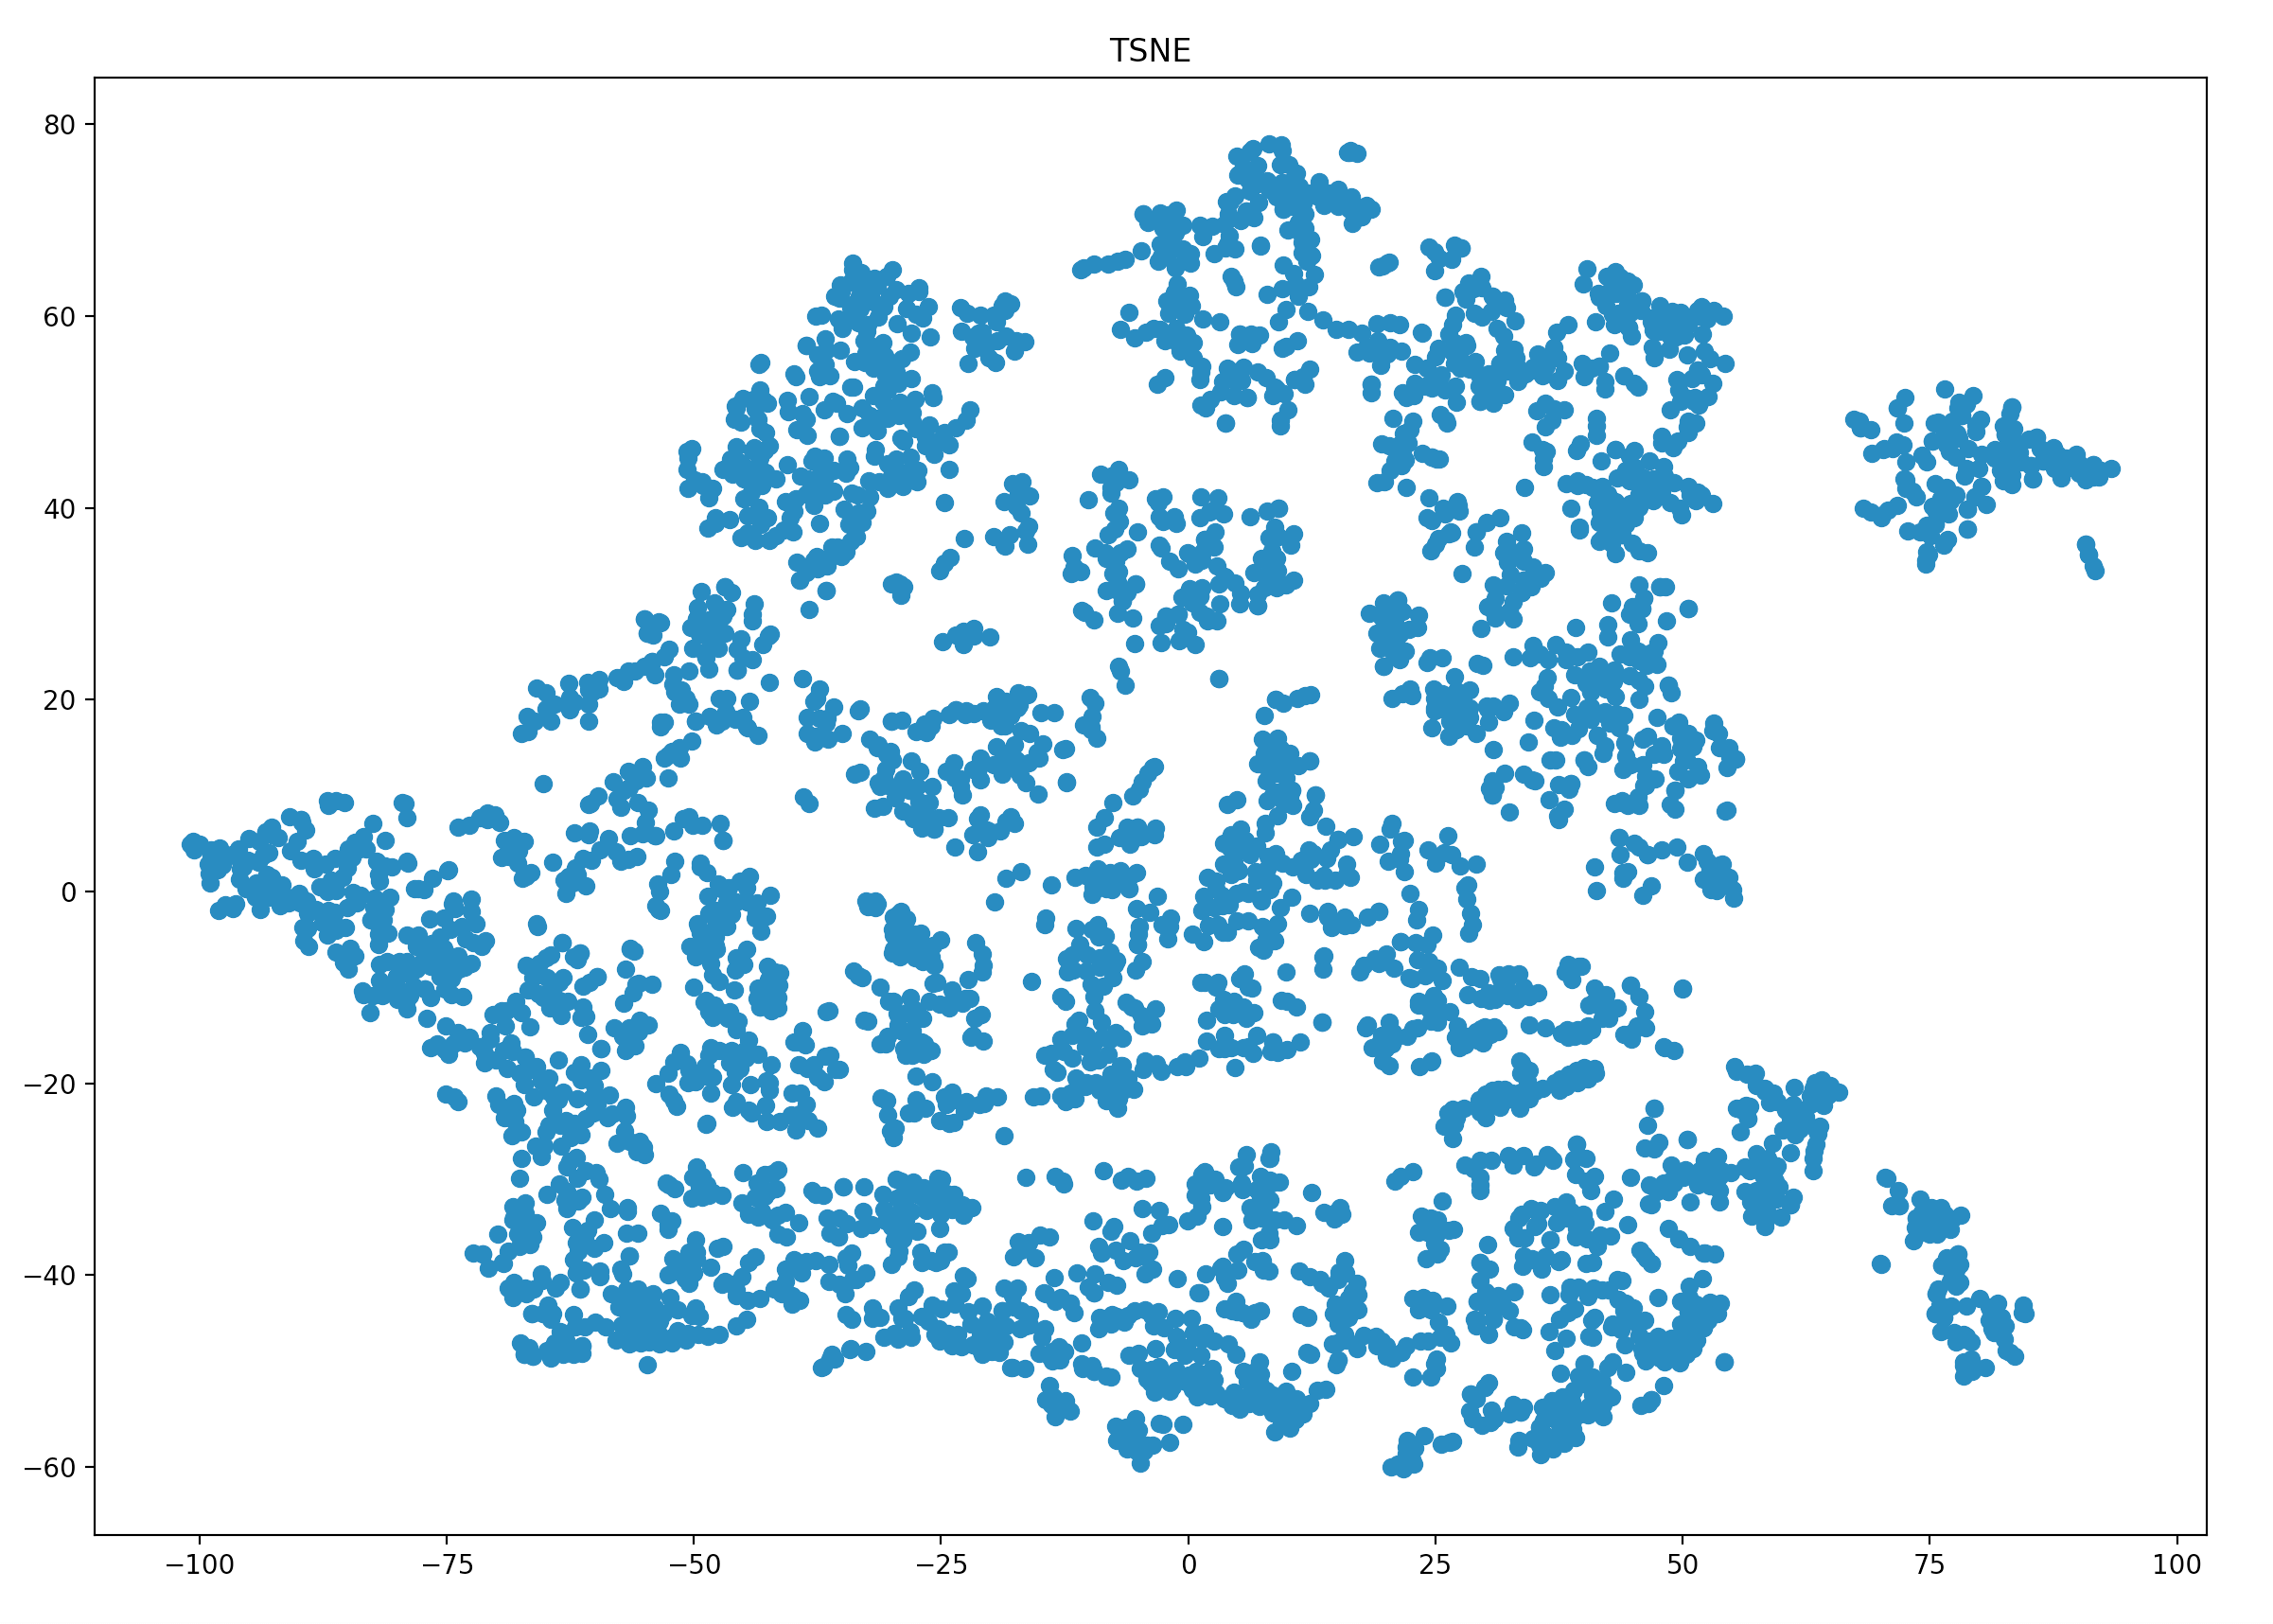
\includegraphics[width=0.9\textwidth]{./images/tsneParametersTest/learningRate/lr400-3hTSNE.png}
  % \caption{}
  % \label{figure:}
  \end{subfigure}%
  \begin{subfigure}{.5\textwidth}
    \centering
    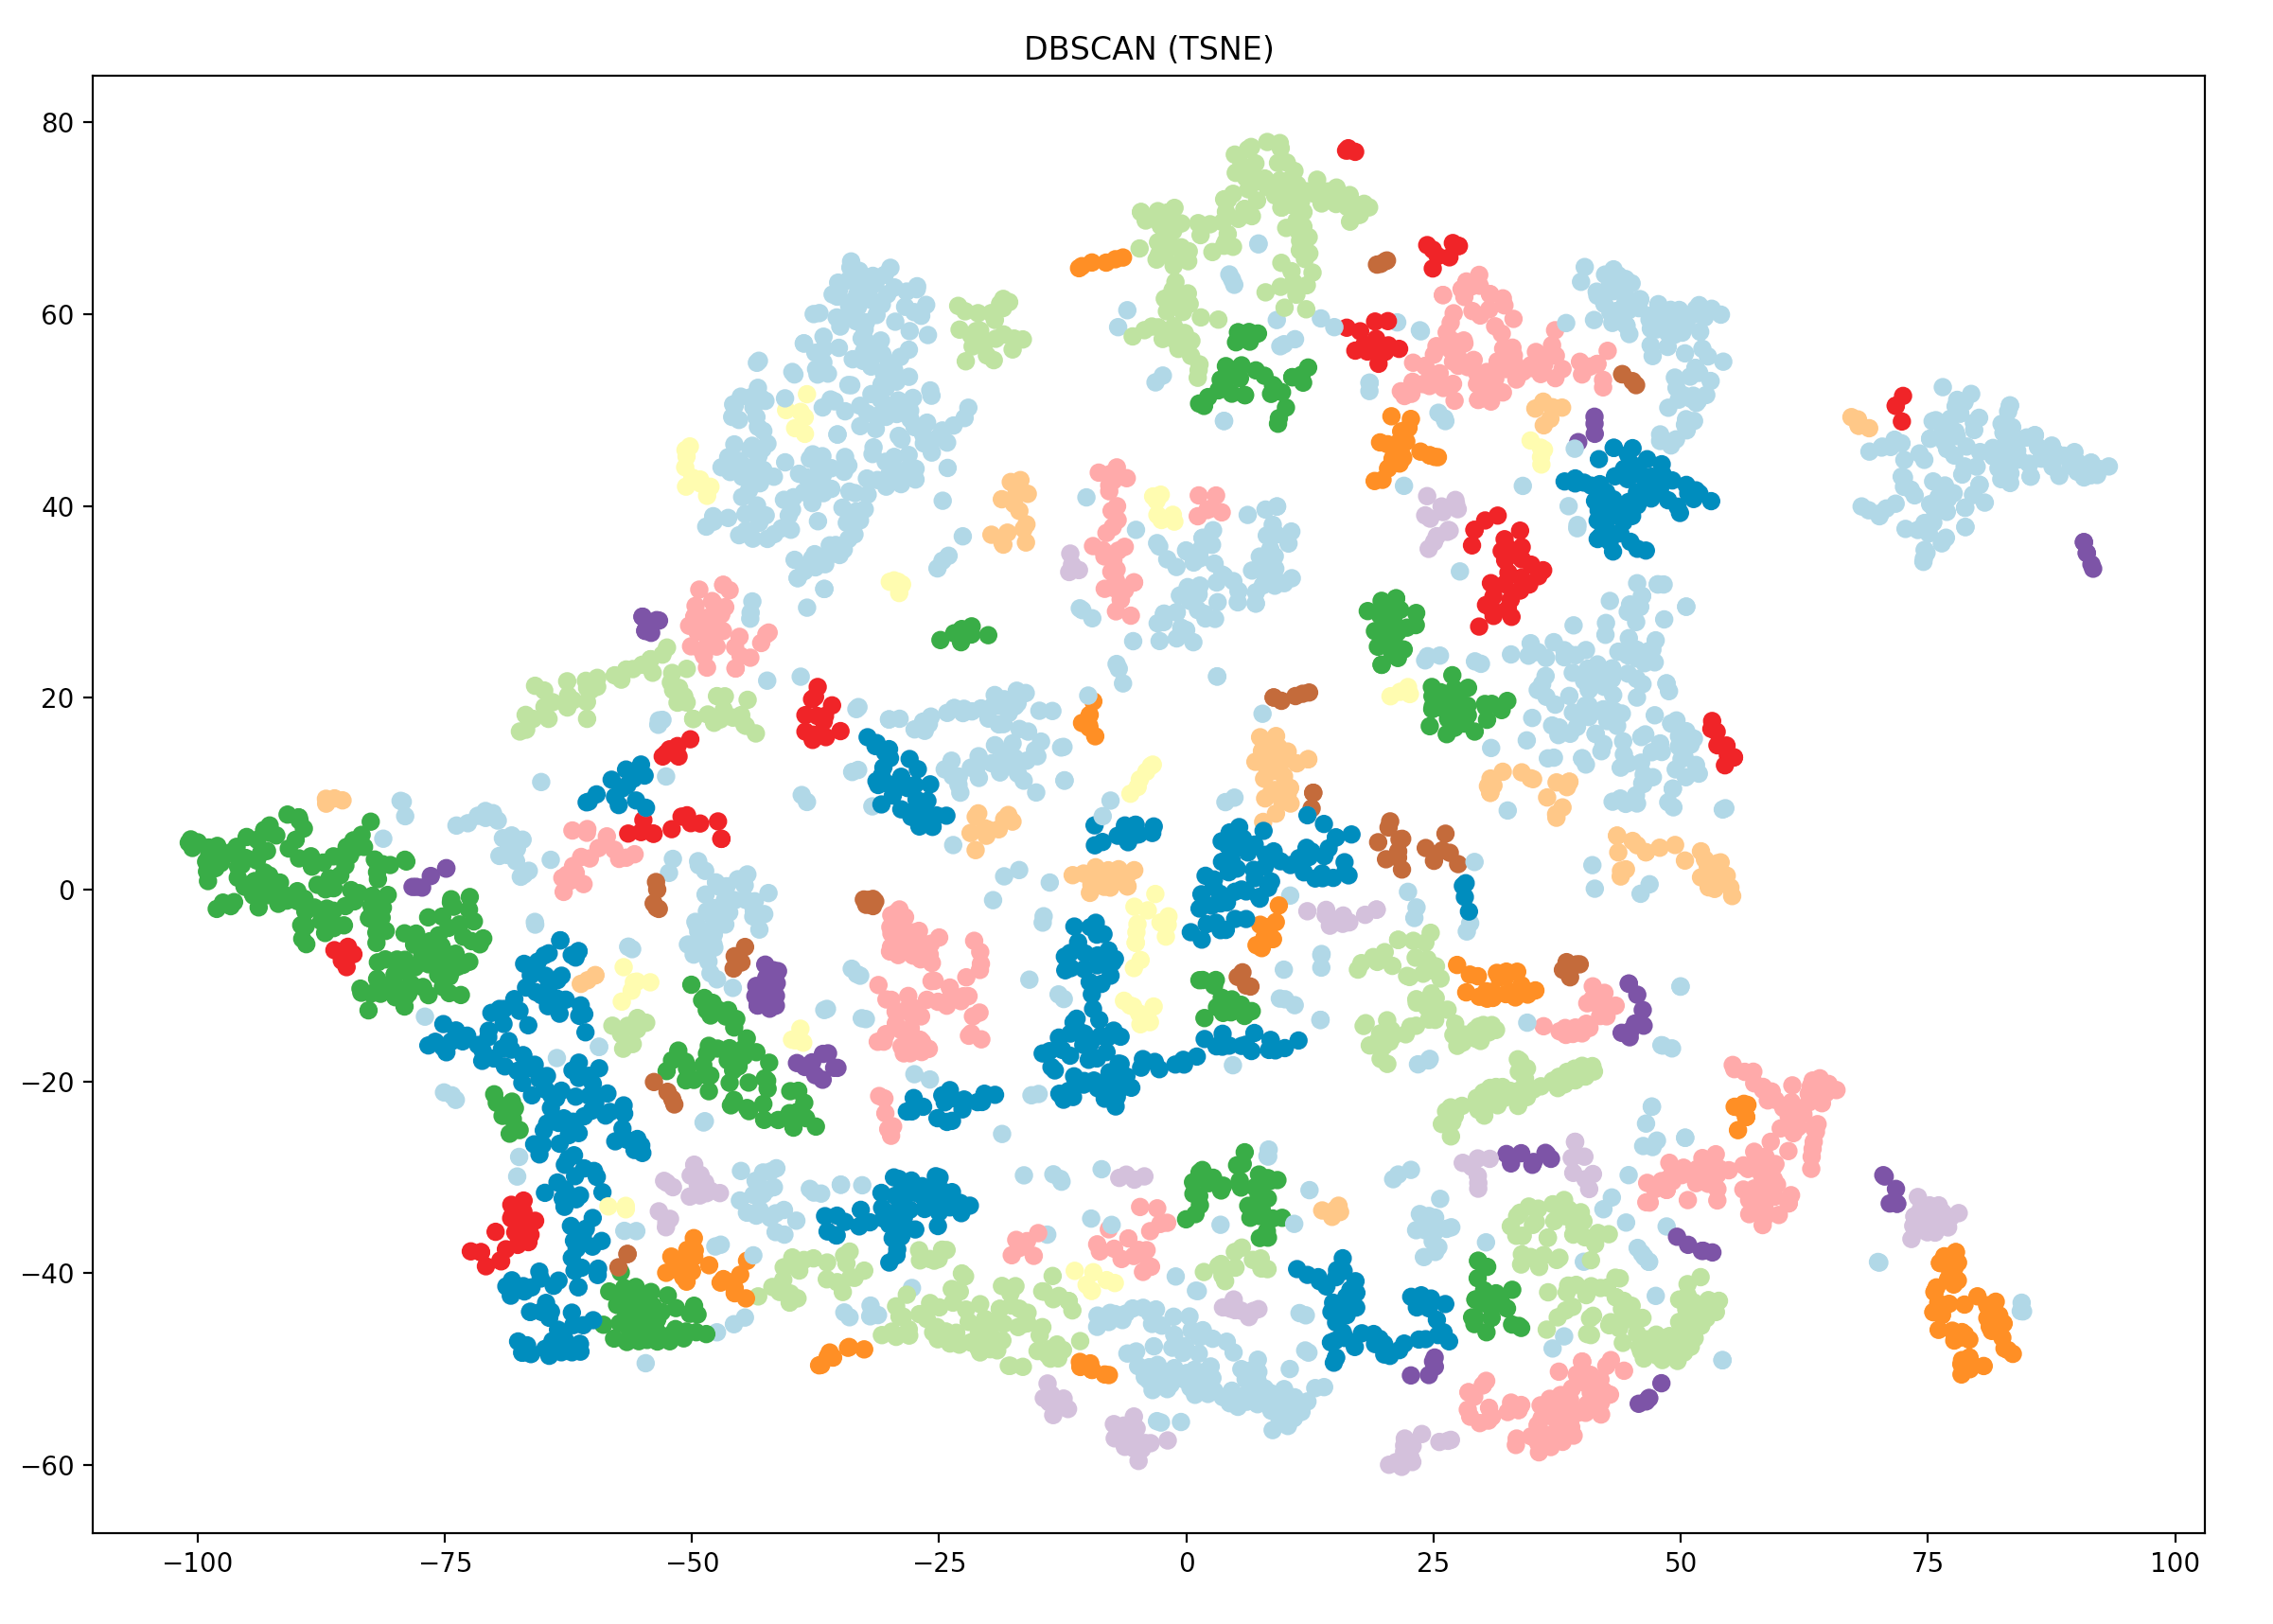
\includegraphics[width=0.9\textwidth]{./images/tsneParametersTest/learningRate/lr400-3hDBSCAN.png}
    % \caption{}
    % \label{figure:}
	\end{subfigure}
	\caption{\textbf{3h} data files, t-SNE calculated with the following parameters: perplexity=40, n\_iter=5000, \textbf{learning\_rate=400}}
  \label{figure:3hlr400TSNE}
\end{figure}


%------------------ LEARNING RATE 600: ------------------
\subsubsection{Learning Rate = 600}
% -- 1h, lr 600 --
\begin{figure}[H]
  \centering
  \begin{subfigure}{.5\textwidth}
    \centering
    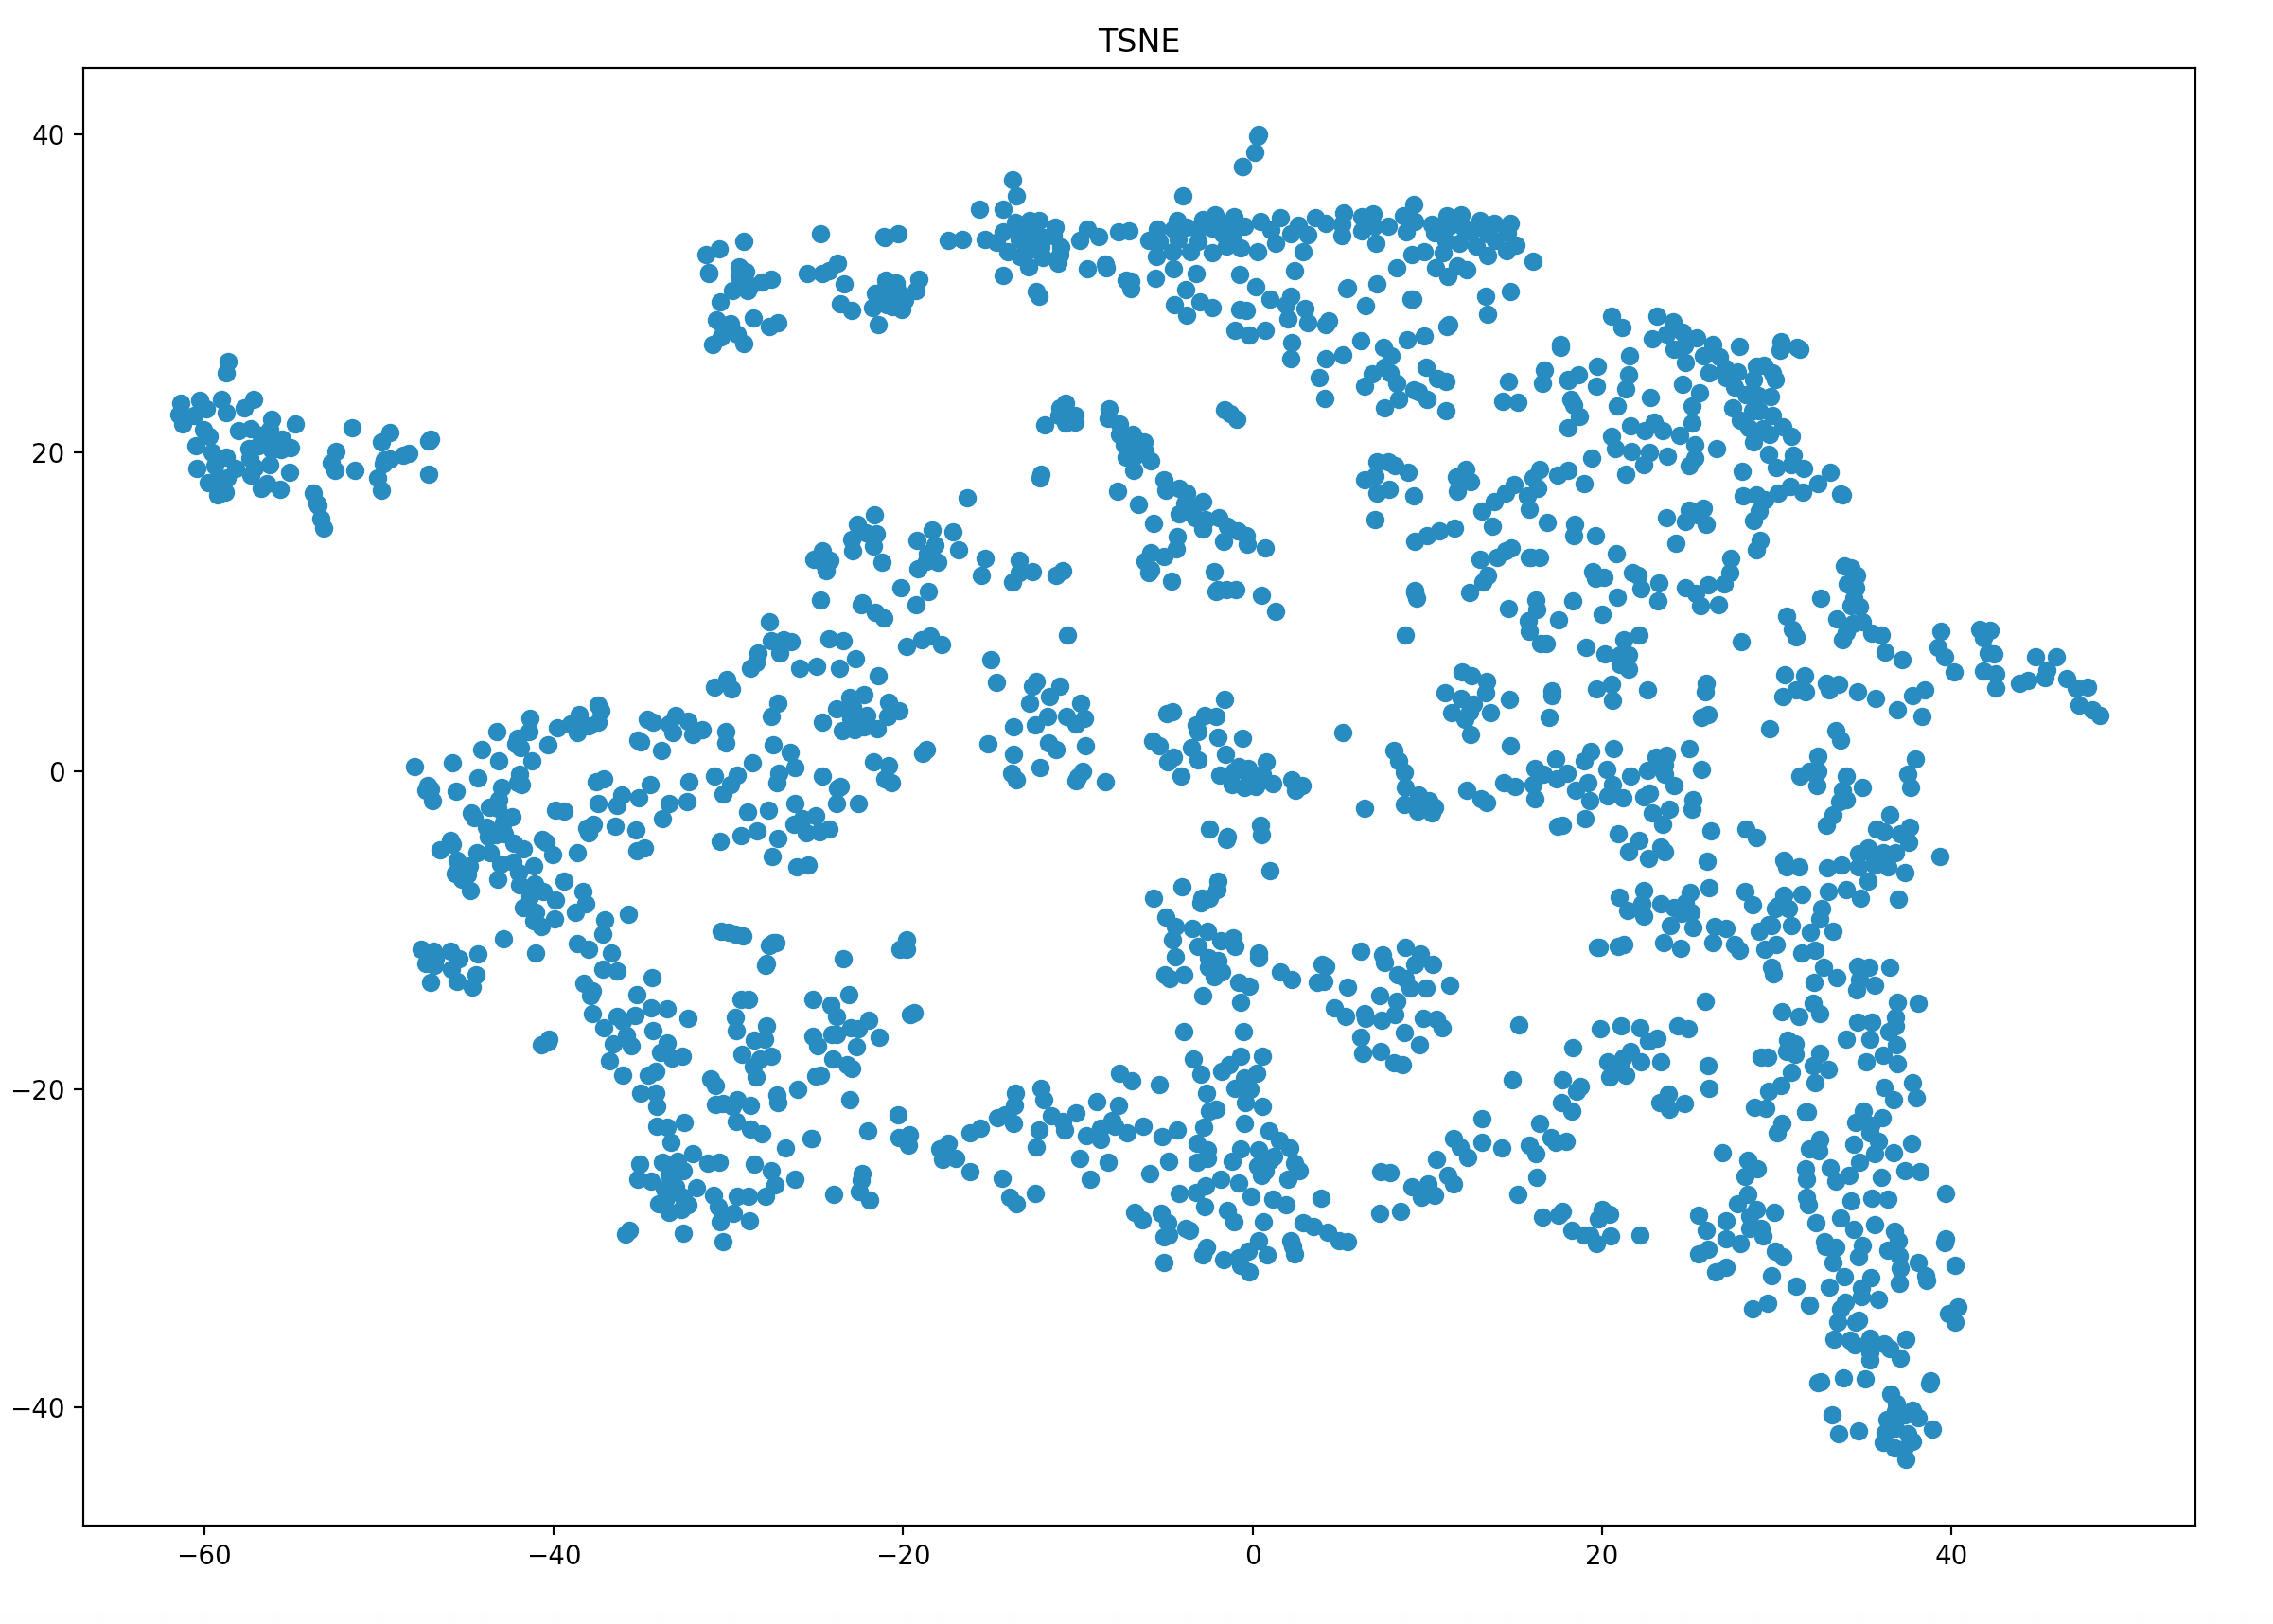
\includegraphics[width=0.9\textwidth]{./images/tsneParametersTest/learningRate/lr600-1hTSNE.png}
  % \caption{}
  % \label{figure:}
  \end{subfigure}%
  \begin{subfigure}{.5\textwidth}
    \centering
    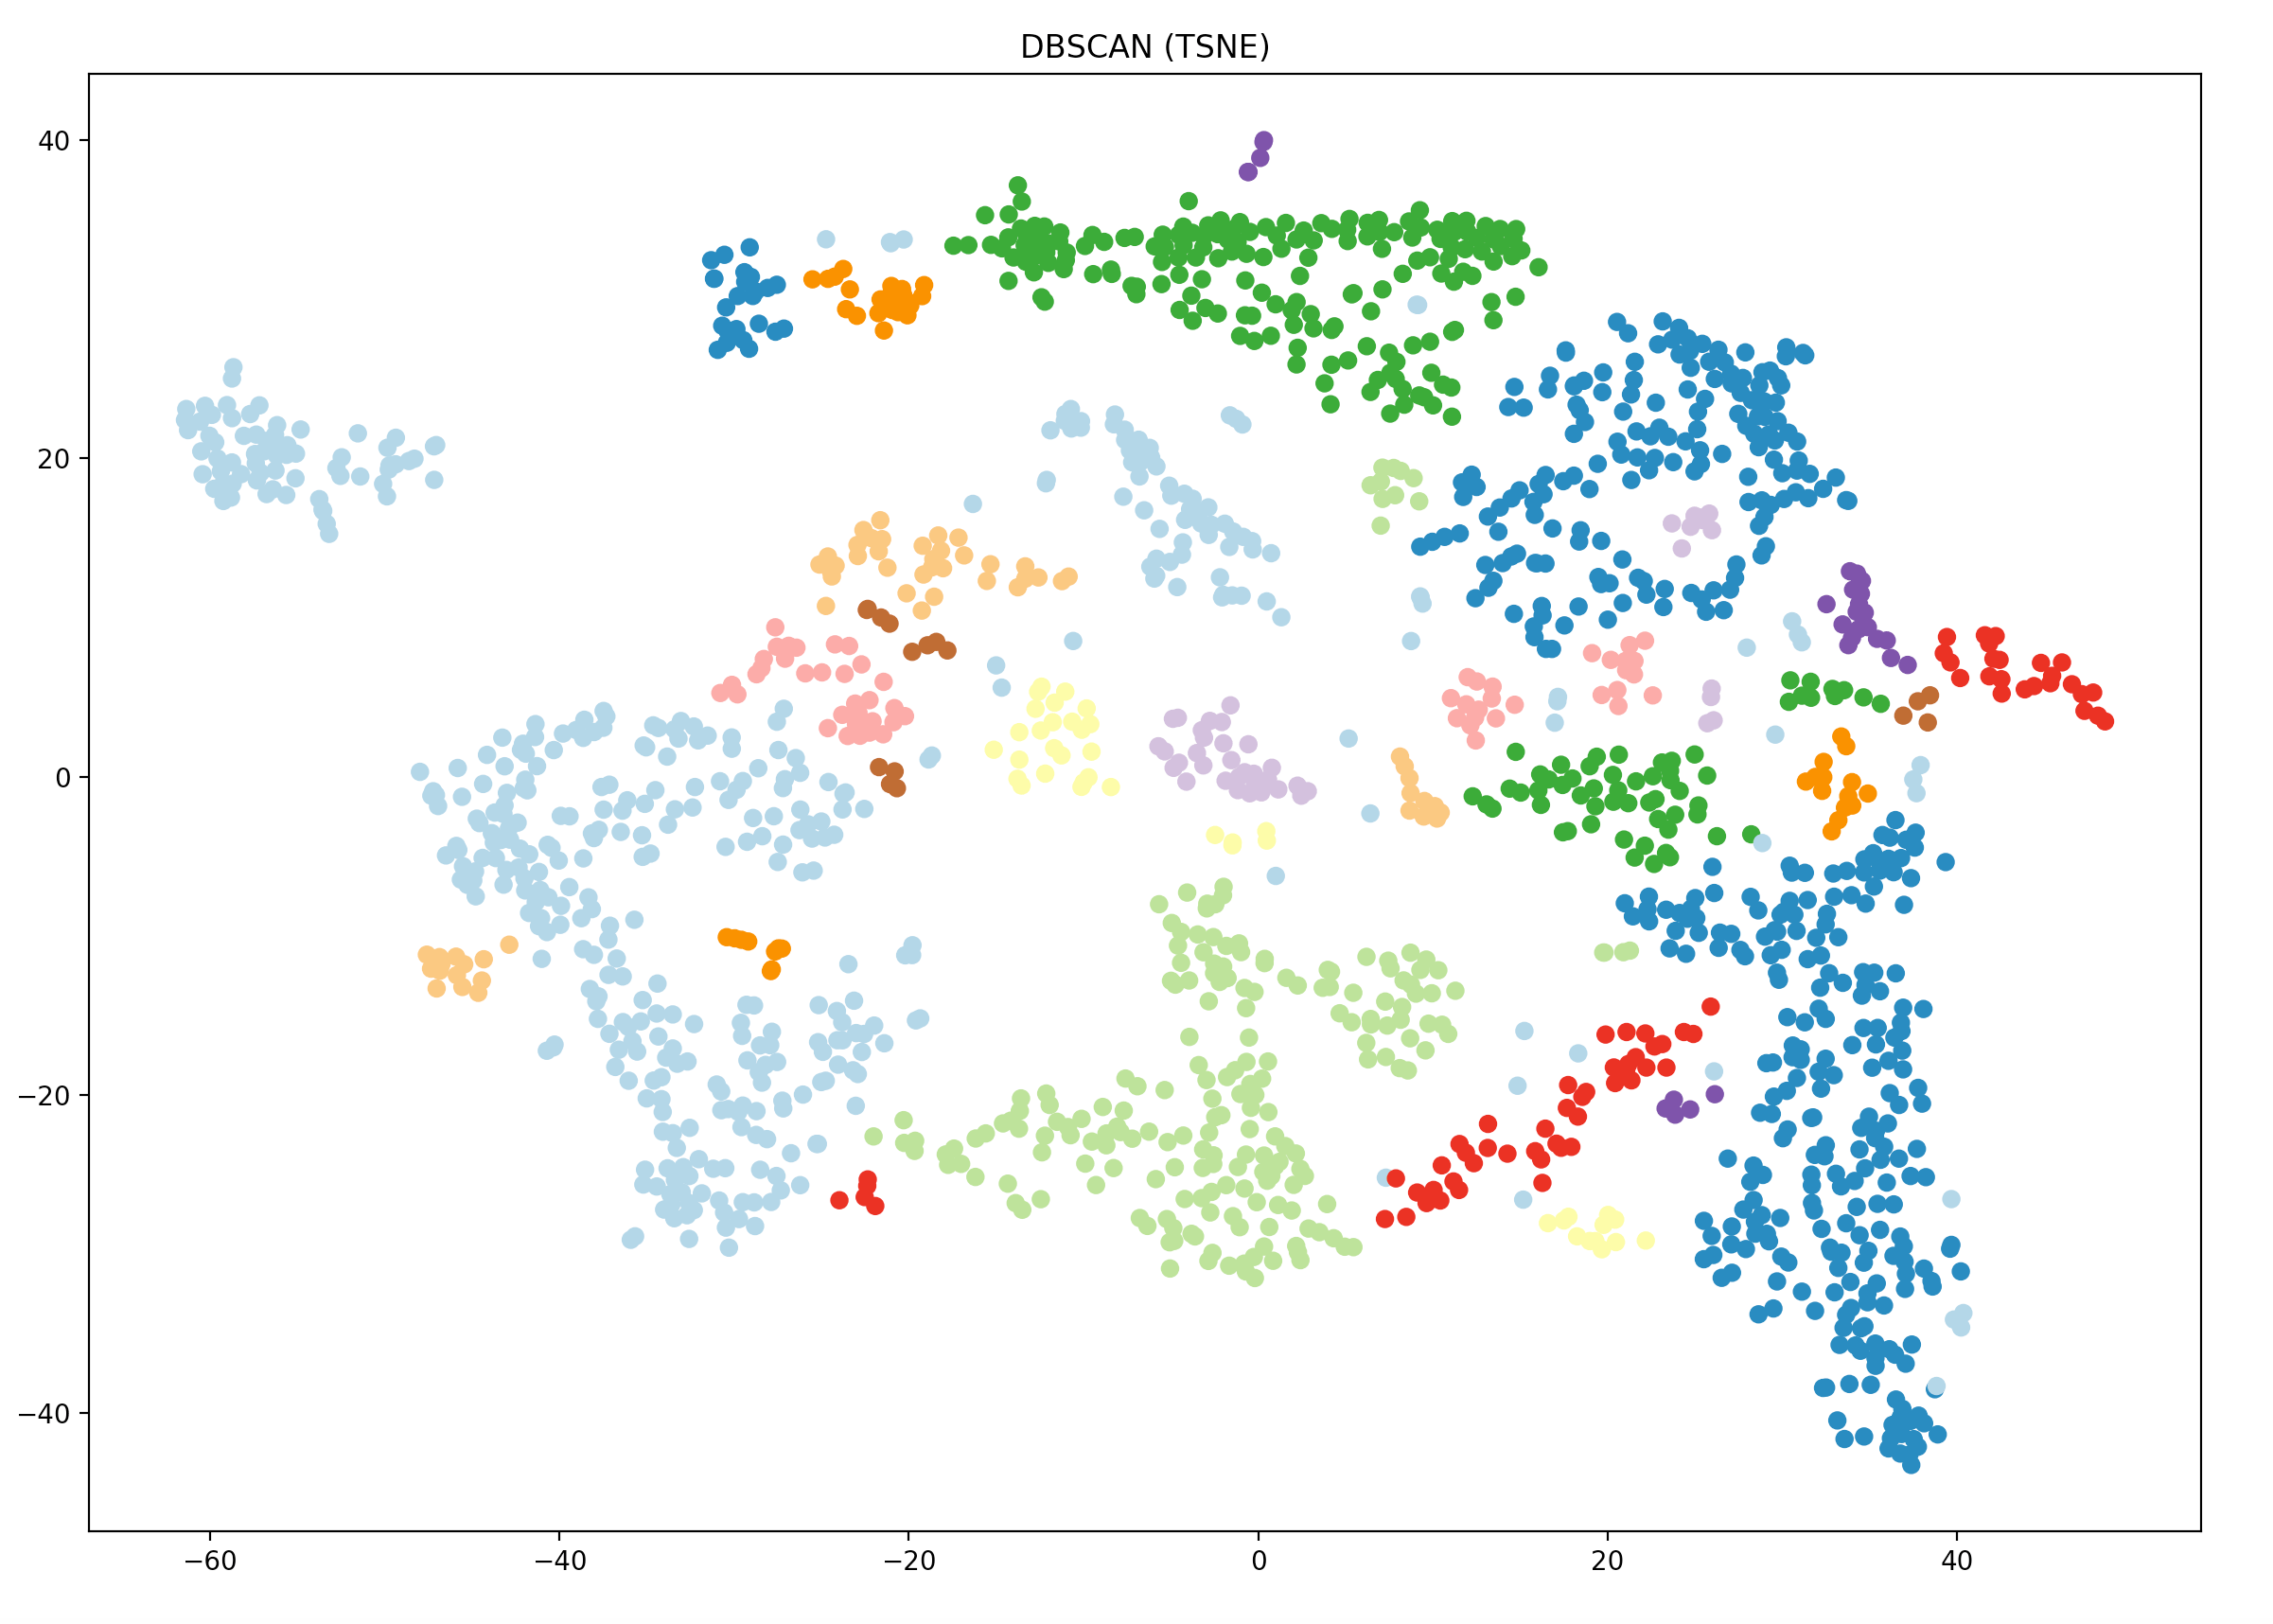
\includegraphics[width=0.9\textwidth]{./images/tsneParametersTest/learningRate/lr600-1hDBSCAN.png}
    % \caption{}
    % \label{figure:}
  \end{subfigure}
	\caption{\textbf{1h} data files, t-SNE calculated with the following parameters: perplexity=40, n\_iter=5000, \textbf{learning\_rate=600}}
	\label{figure:1hlr600TSNE}
\end{figure}

% -- 3h, lr 600 --
\begin{figure}[H]
	\centering
	
  \centering
	\begin{subfigure}{.5\textwidth}
    \centering
    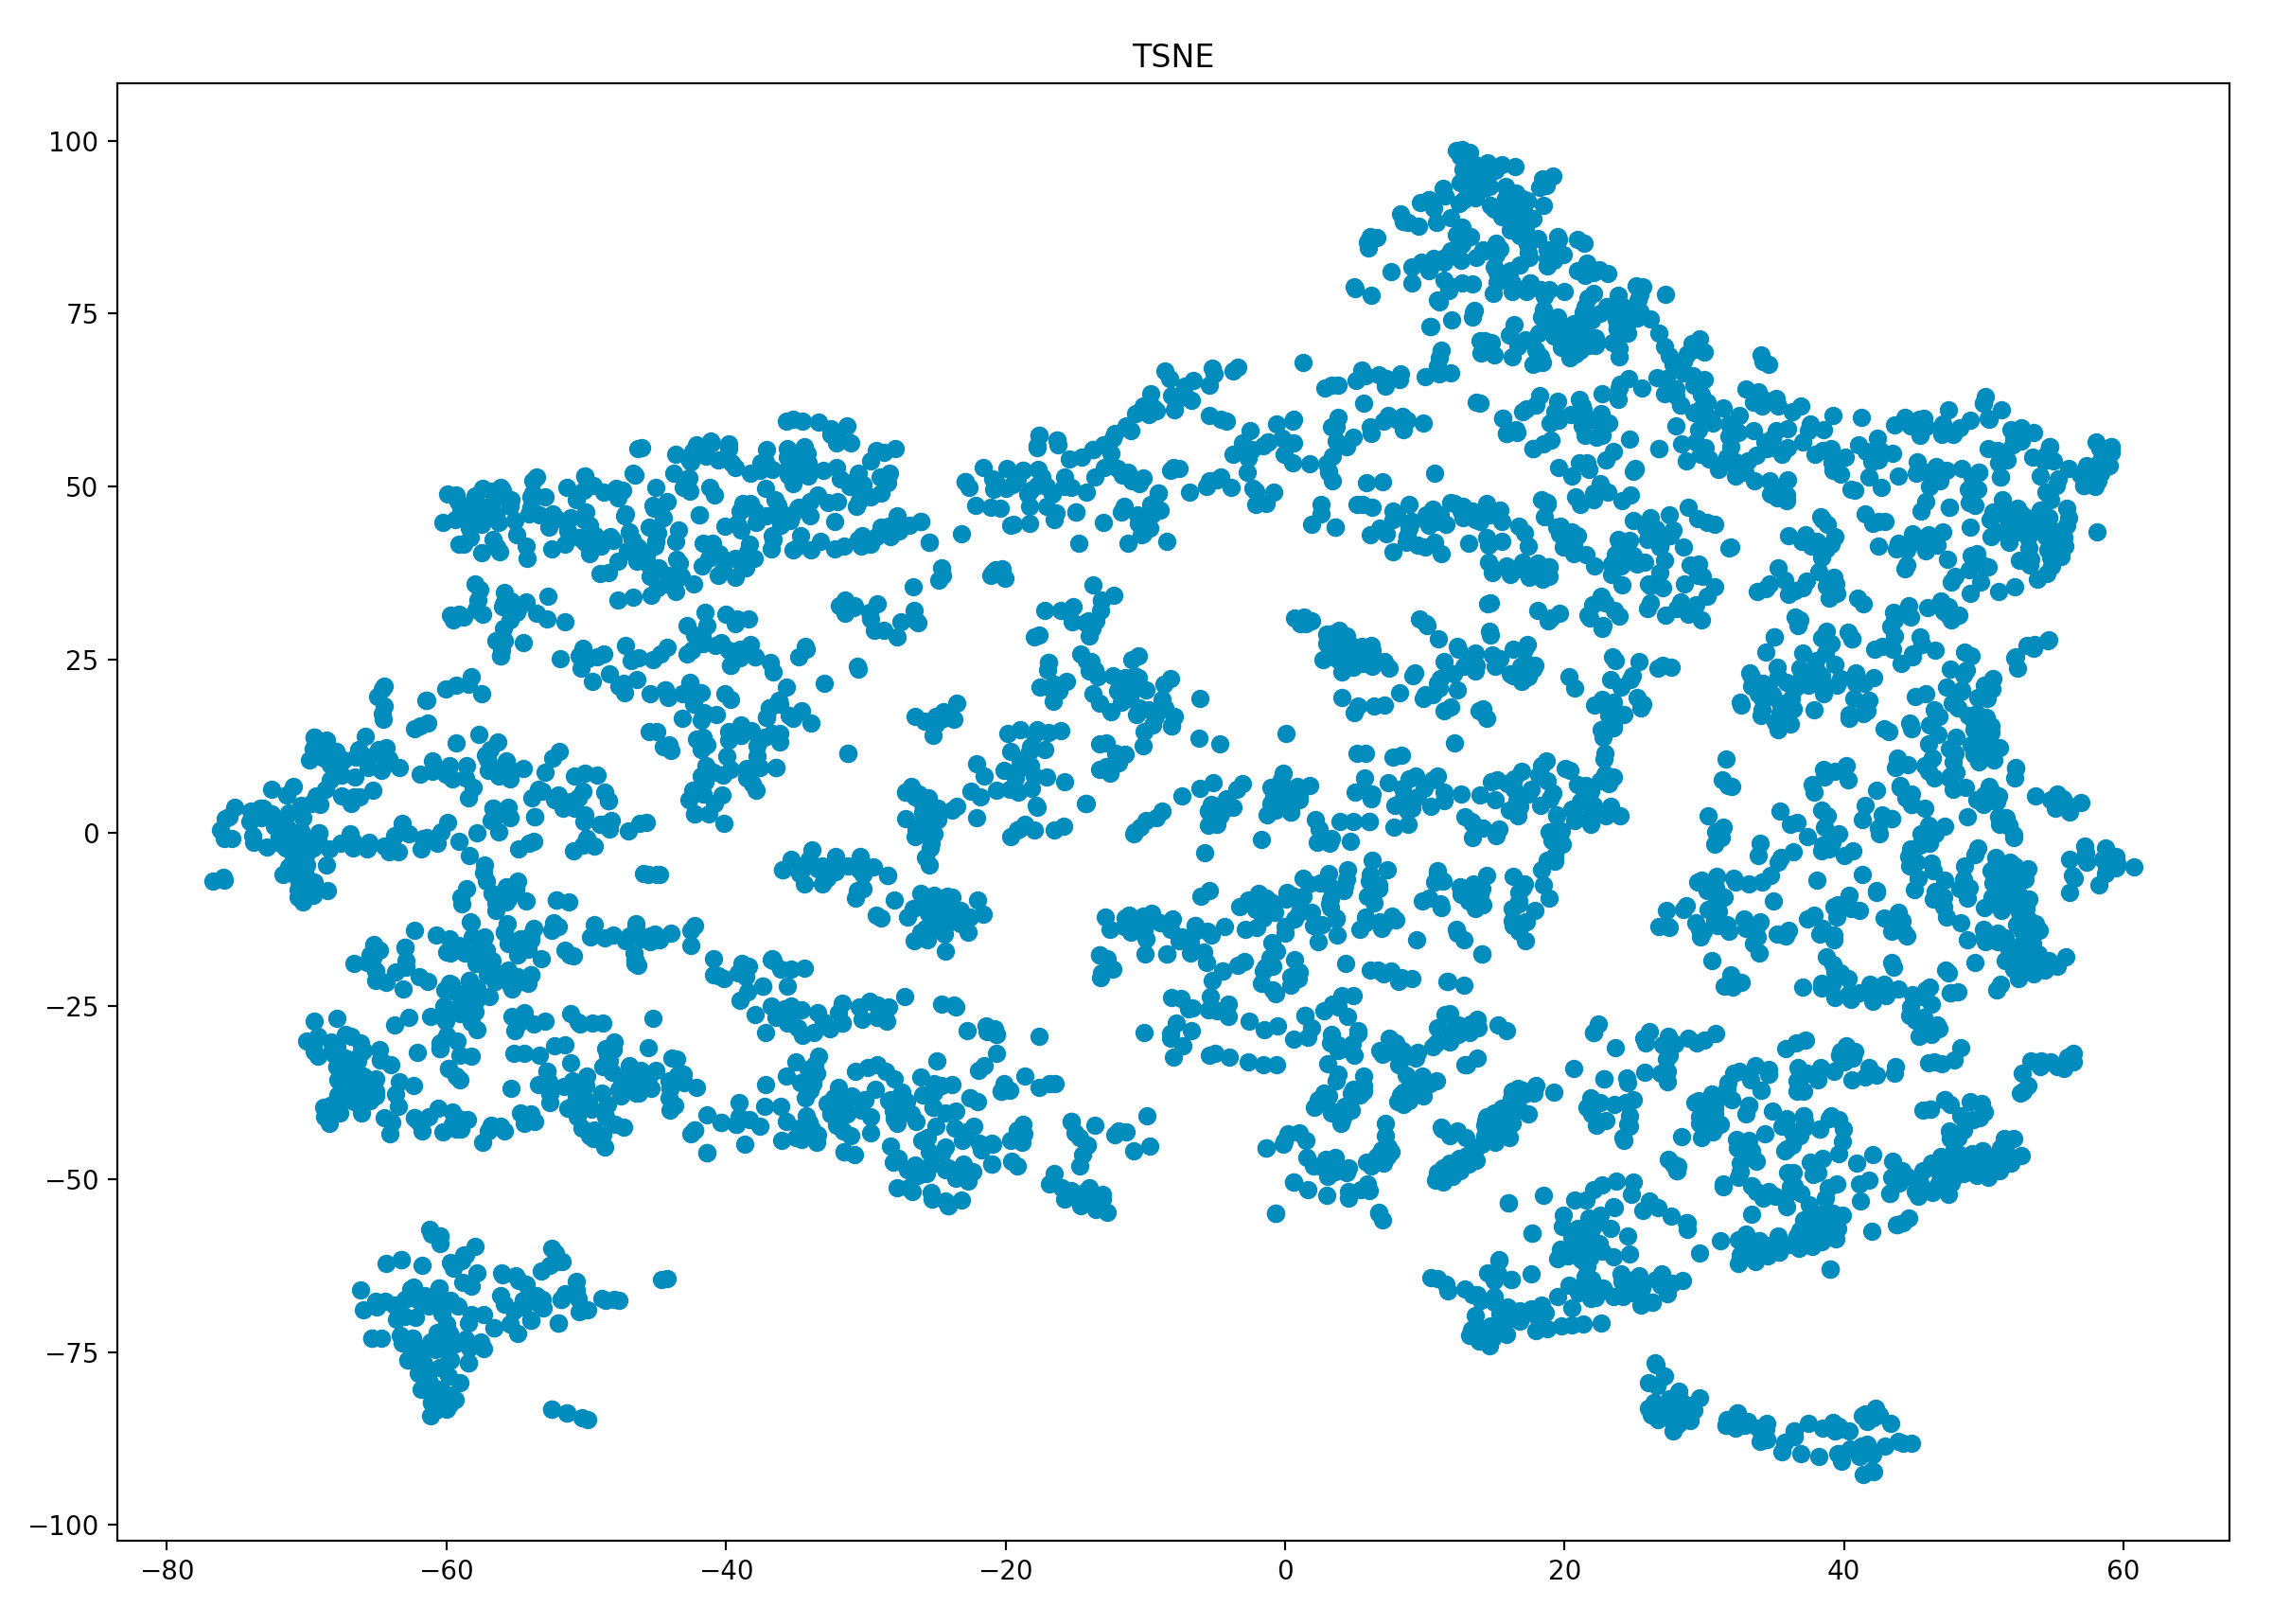
\includegraphics[width=0.9\textwidth]{./images/tsneParametersTest/learningRate/lr600-3hTSNE.png}
  % \caption{}
  % \label{figure:}
  \end{subfigure}%
  \begin{subfigure}{.5\textwidth}
    \centering
    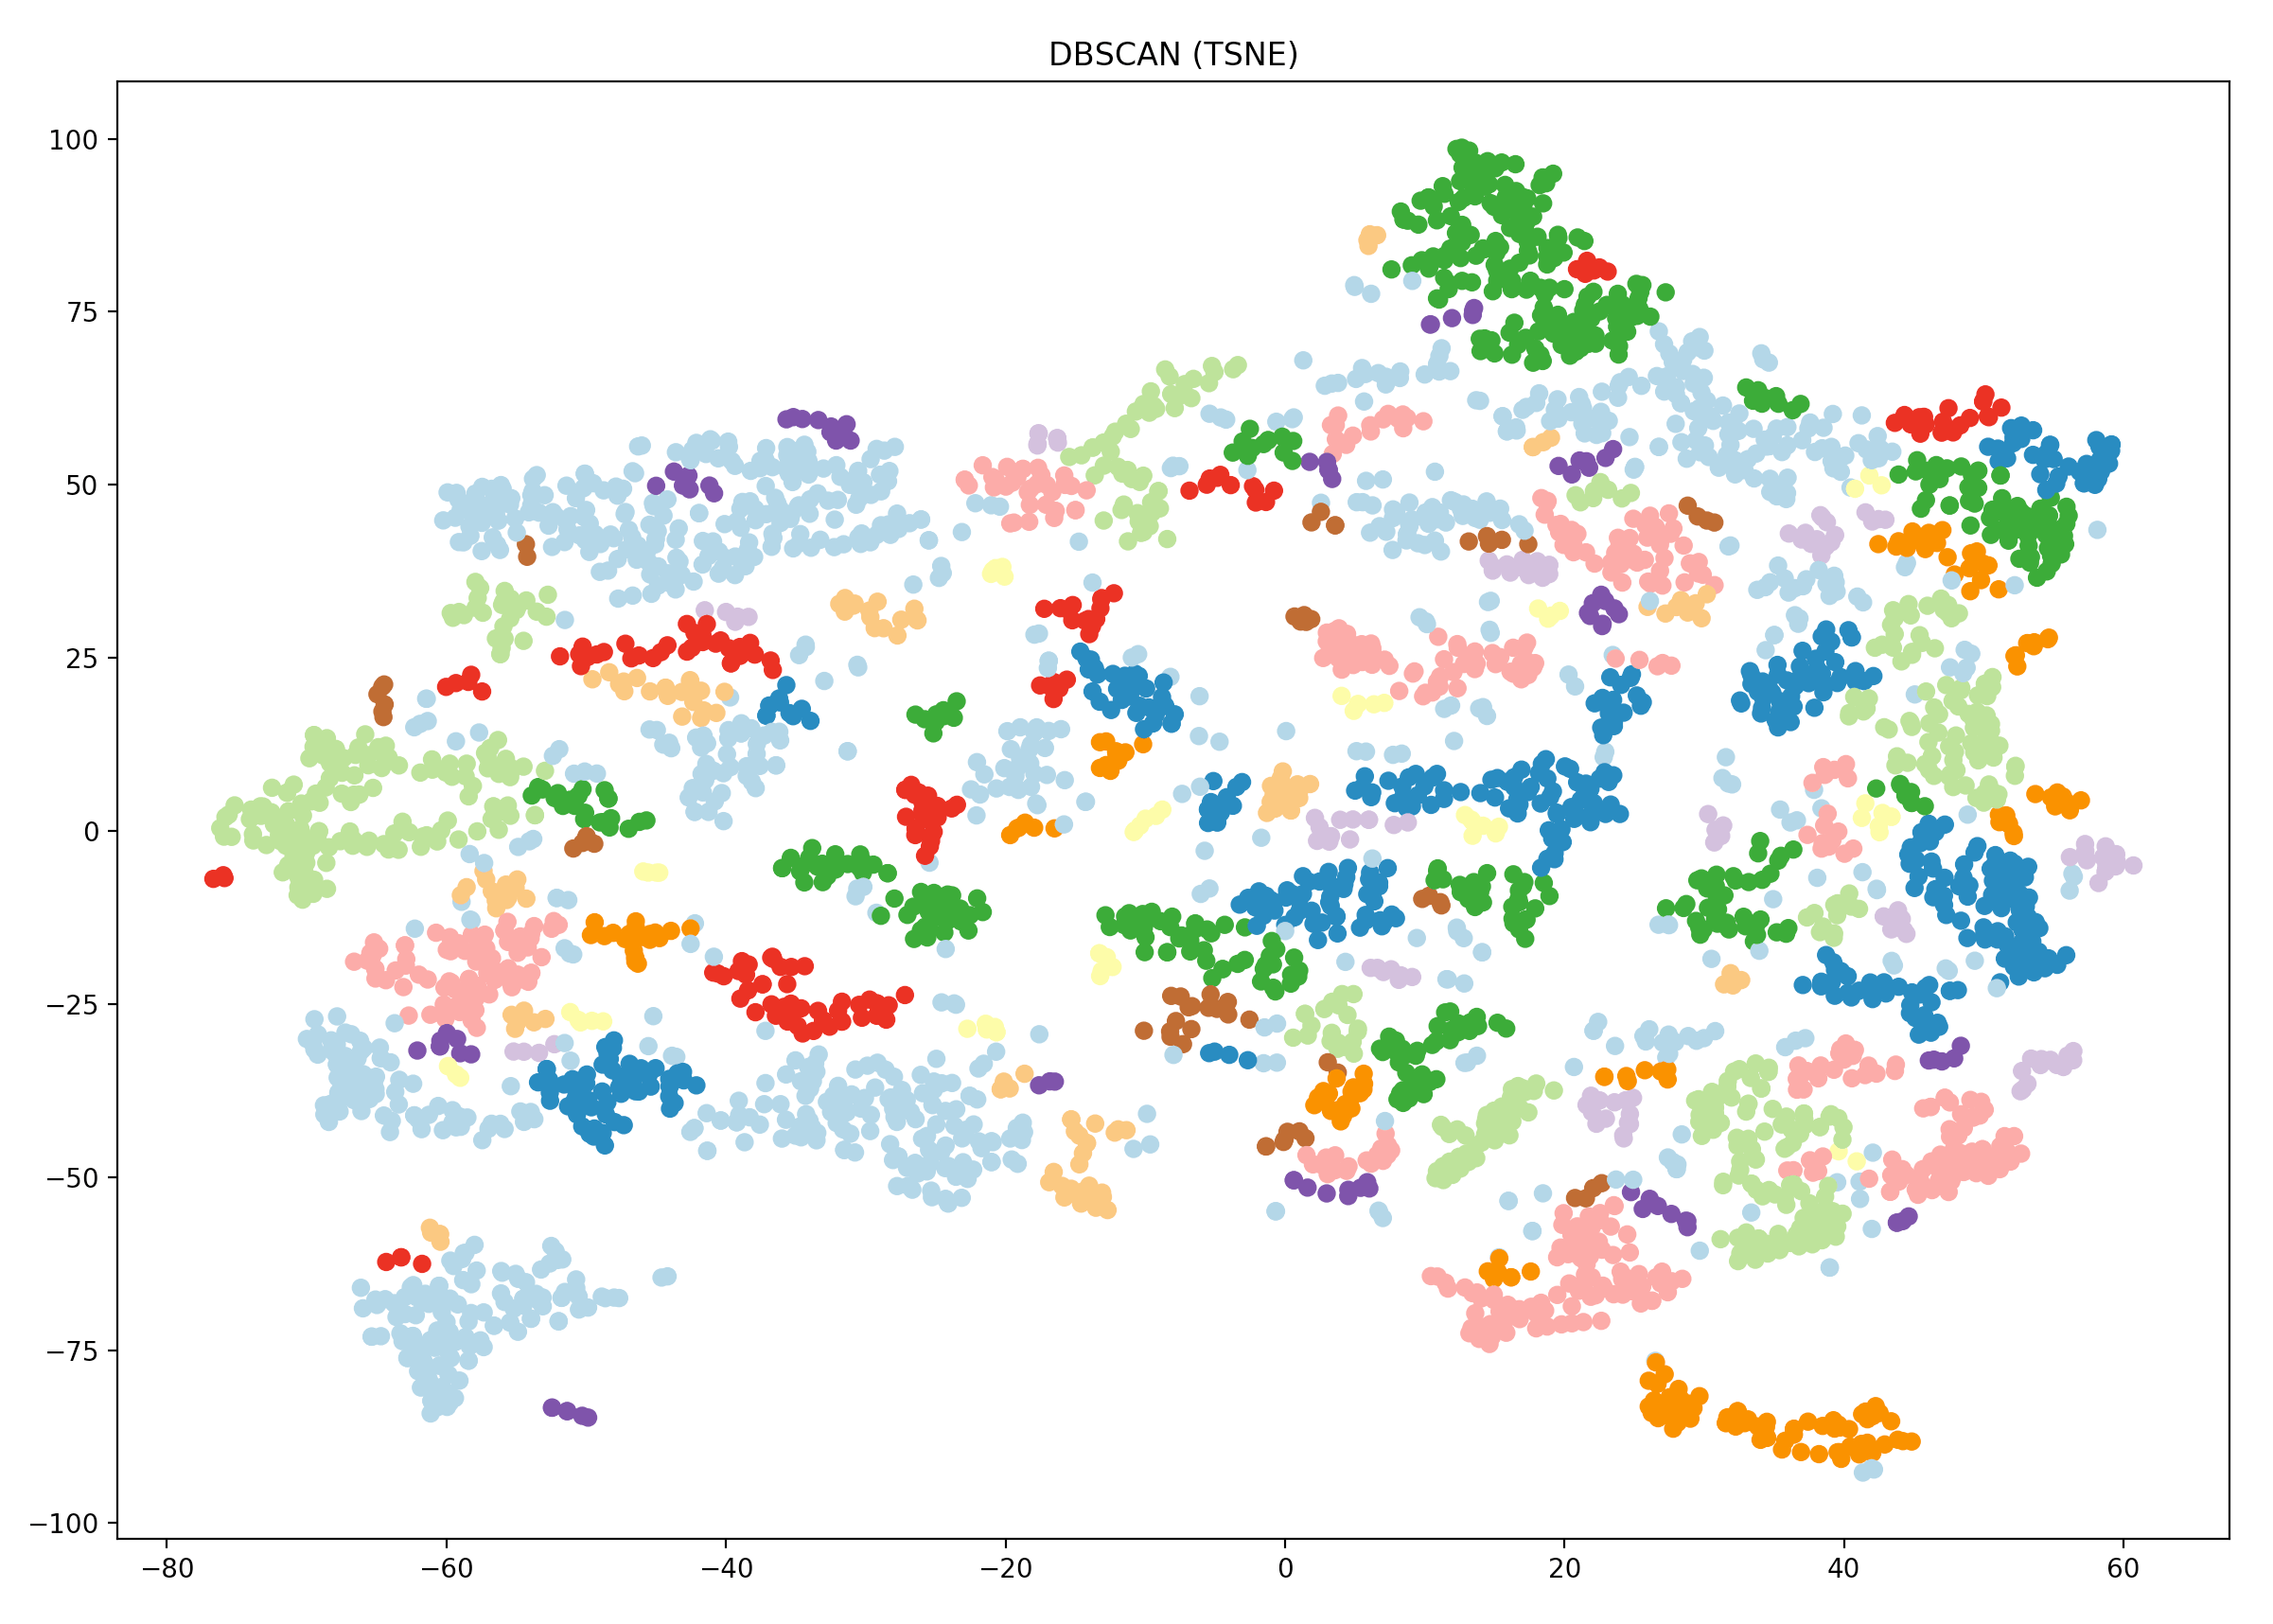
\includegraphics[width=0.9\textwidth]{./images/tsneParametersTest/learningRate/lr600-3hDBSCAN.png}
    % \caption{}
    % \label{figure:}
	\end{subfigure}
	\caption{\textbf{3h} data files, t-SNE calculated with the following parameters: perplexity=40, n\_iter=5000, \textbf{learning\_rate=600}}
  \label{figure:3hlr600TSNE}
\end{figure}




%------------------ LEARNING RATE 800: ------------------
\subsubsection{Learning Rate = 800}
% -- 1h, lr 800 --
\begin{figure}[H]
  \centering
  \begin{subfigure}{.5\textwidth}
    \centering
    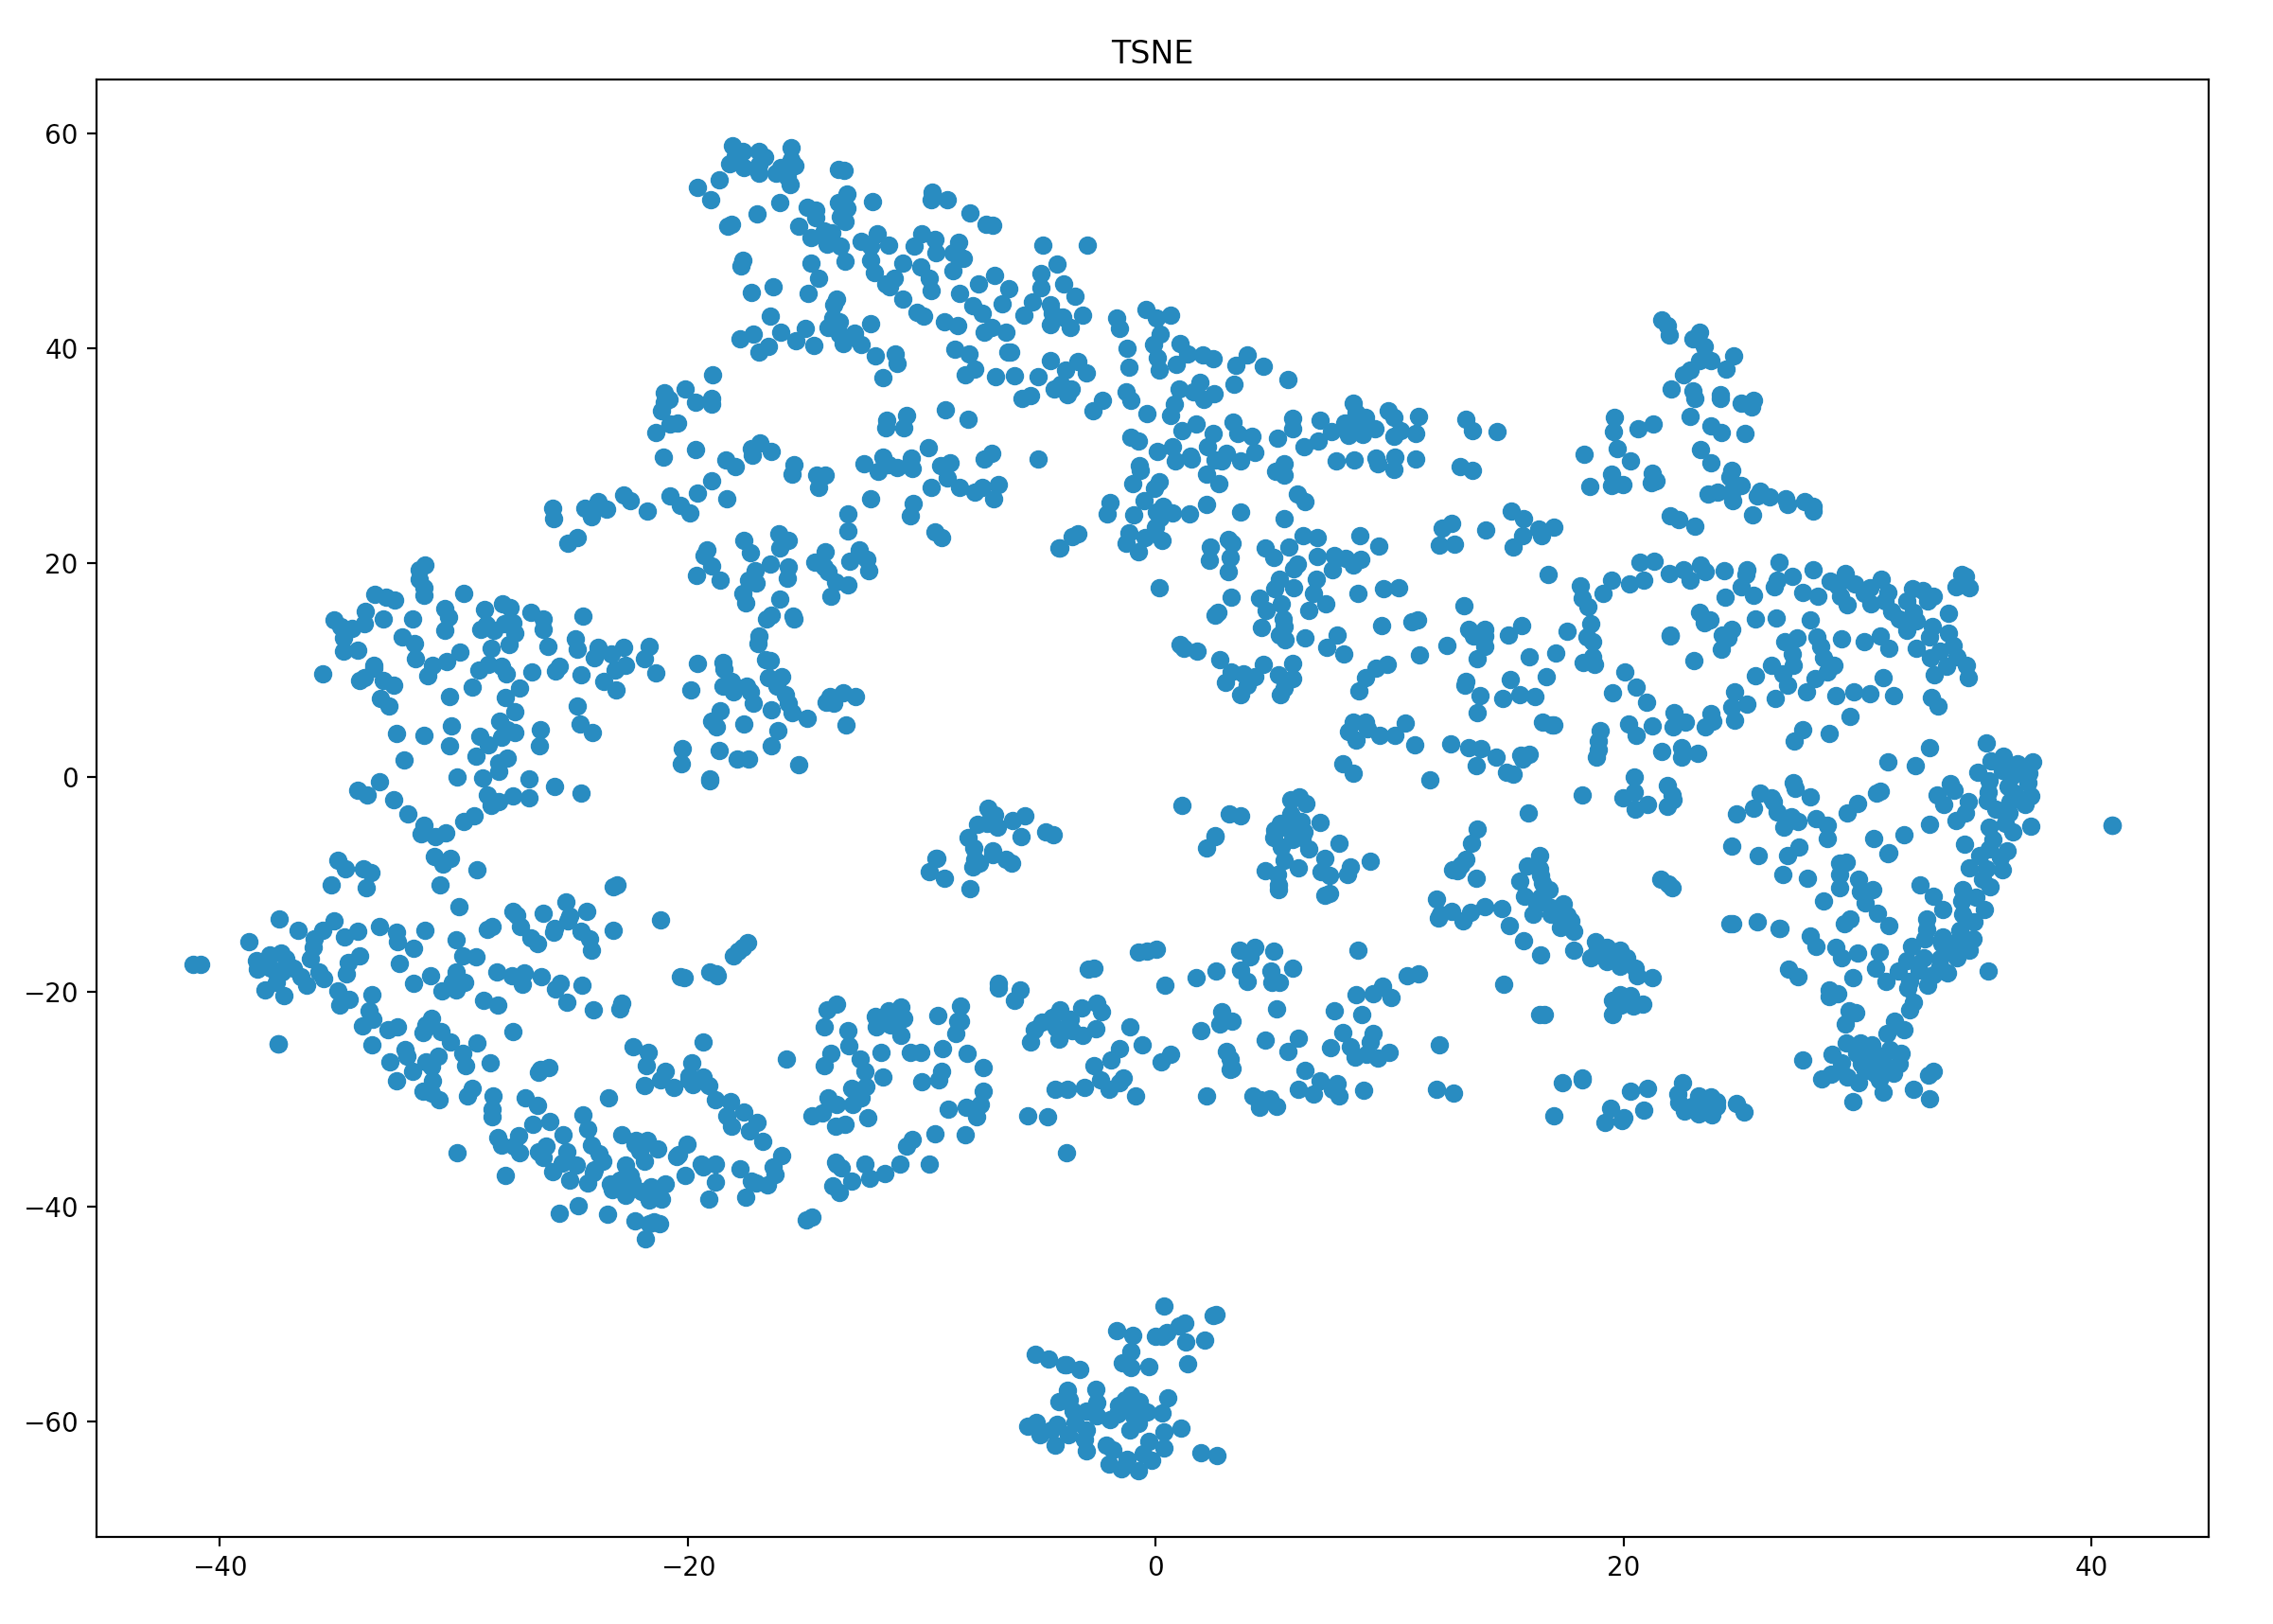
\includegraphics[width=0.9\textwidth]{./images/tsneParametersTest/learningRate/lr800-1hTSNE.png}
  % \caption{}
  % \label{figure:}
  \end{subfigure}%
  \begin{subfigure}{.5\textwidth}
    \centering
    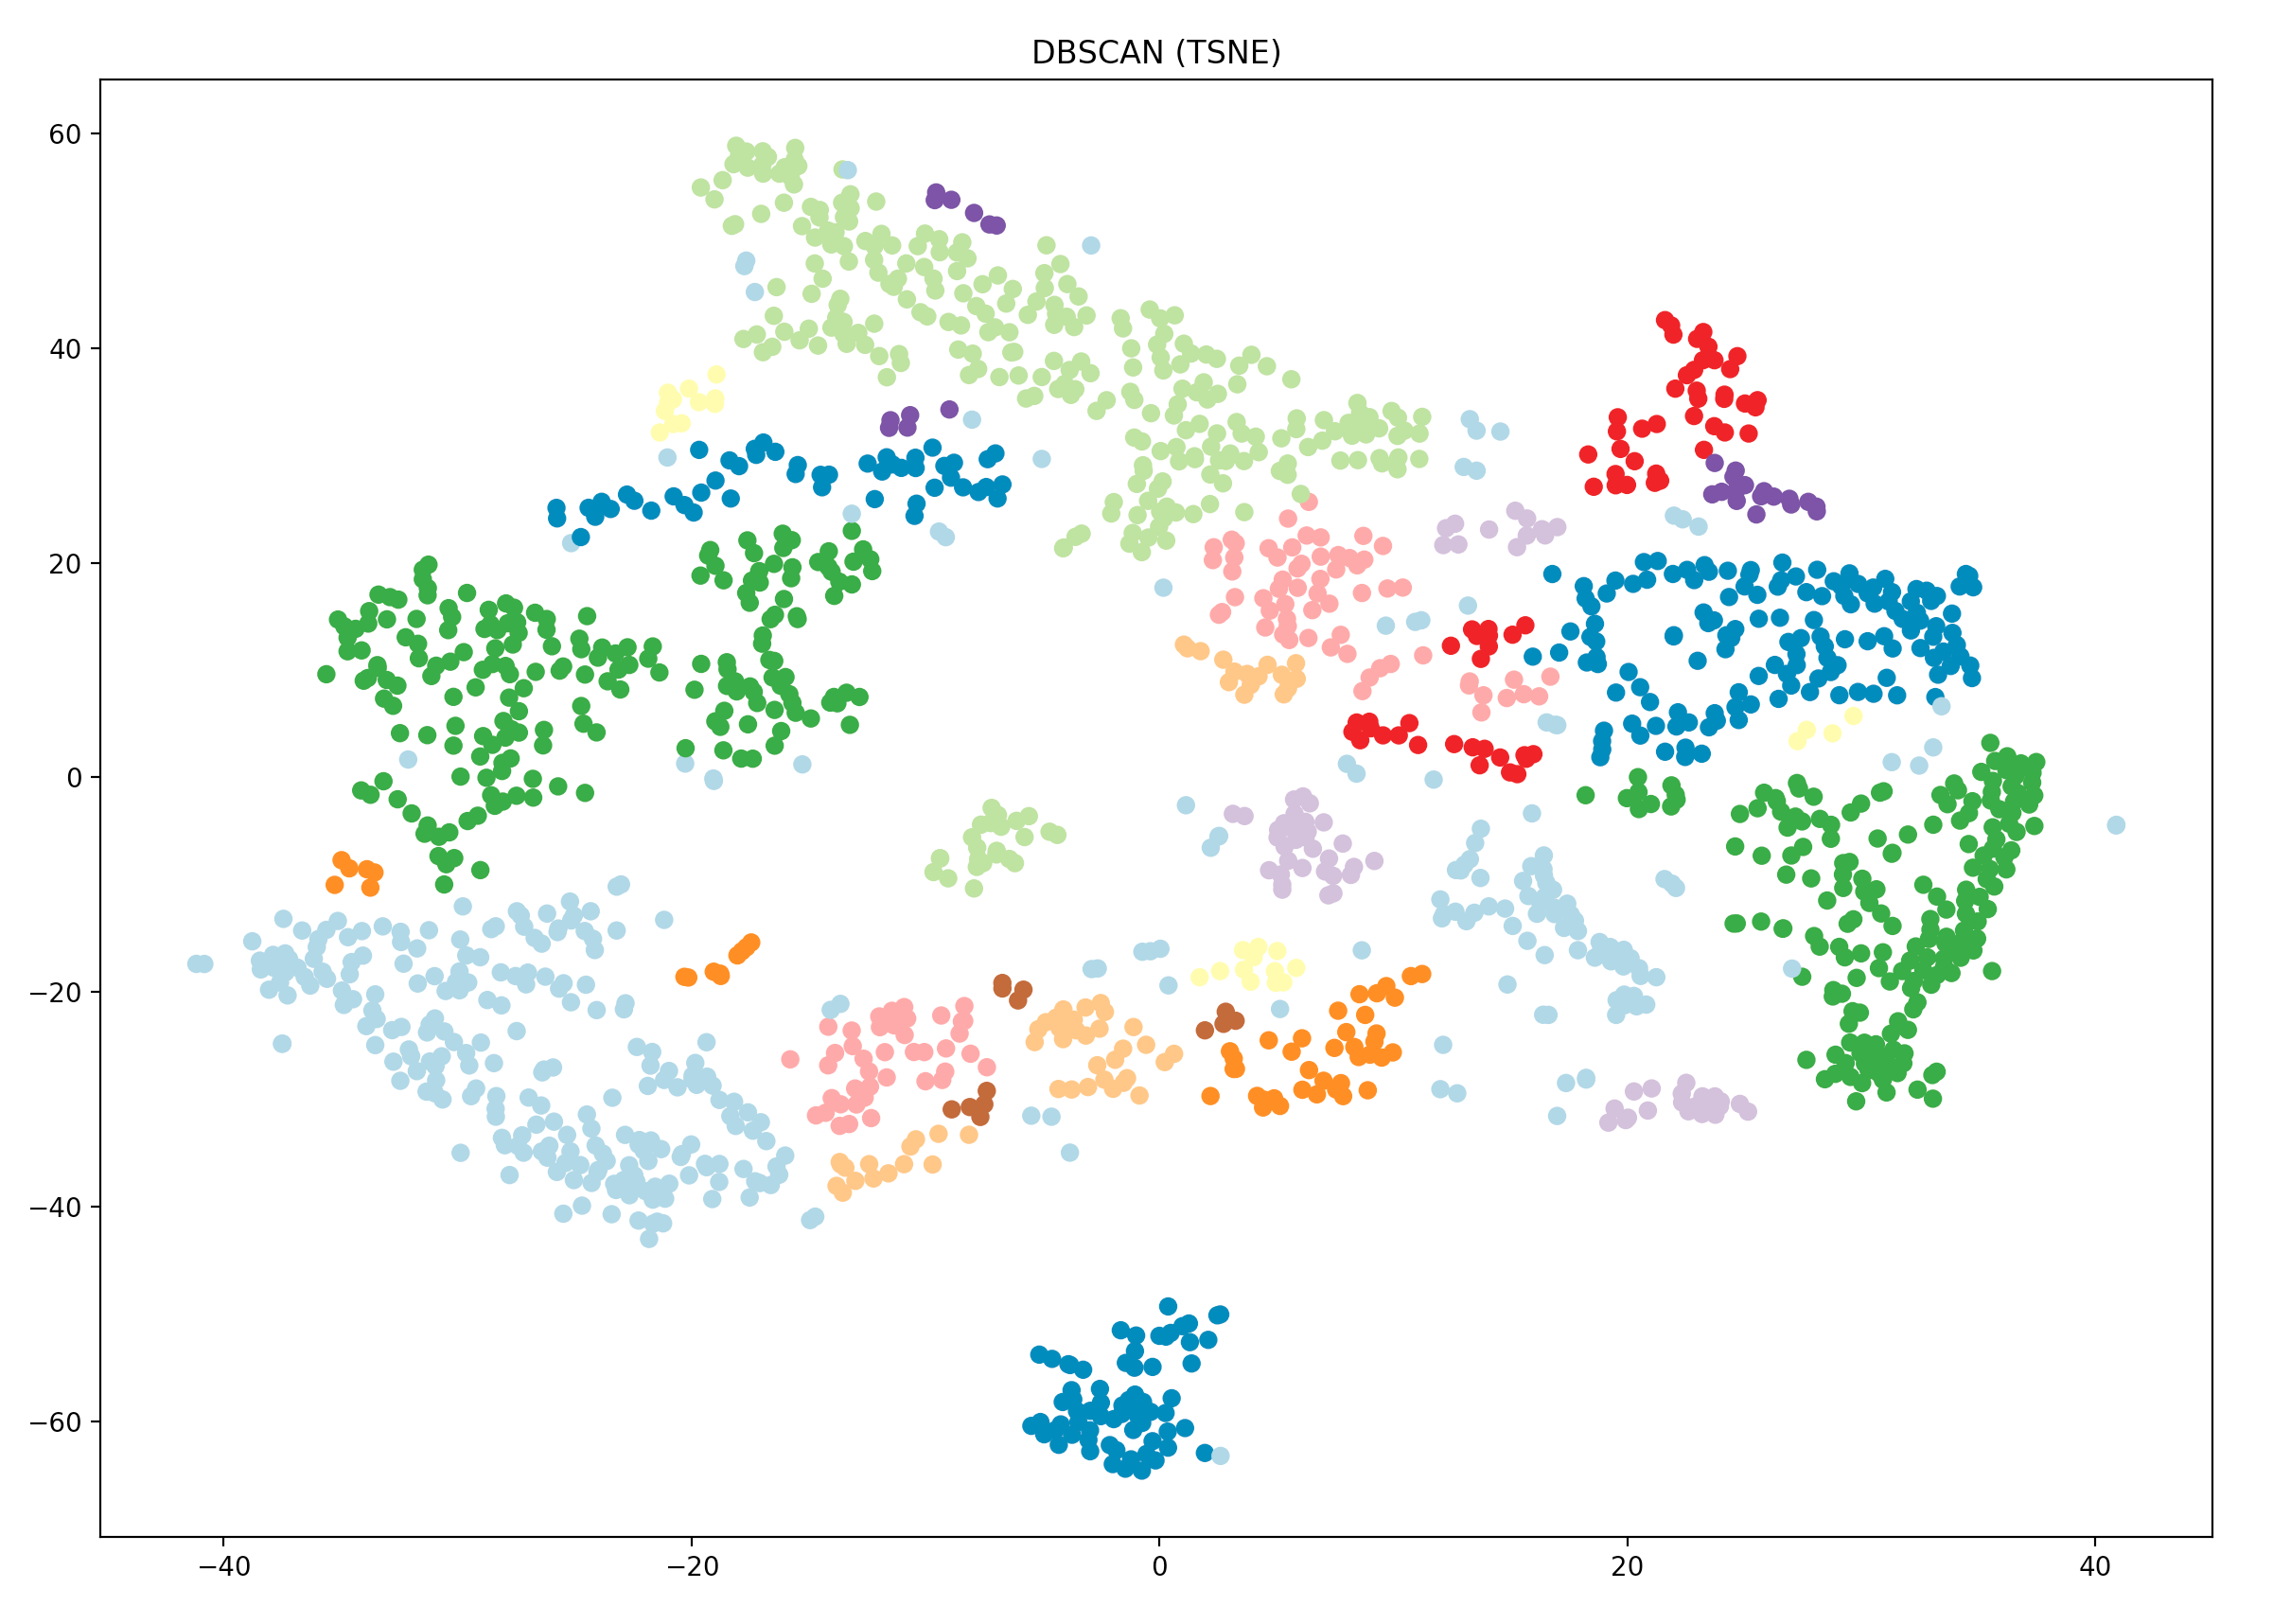
\includegraphics[width=0.9\textwidth]{./images/tsneParametersTest/learningRate/lr800-1hDBSCAN.png}
    % \caption{}
    % \label{figure:}
  \end{subfigure}
	\caption{\textbf{1h} data files, t-SNE calculated with the following parameters: perplexity=40, n\_iter=5000, \textbf{learning\_rate=800}}
	\label{figure:1hlr800TSNE}
\end{figure}

% -- 3h, lr 800 --
\begin{figure}[H]
	\centering
	
  \centering
	\begin{subfigure}{.5\textwidth}
    \centering
    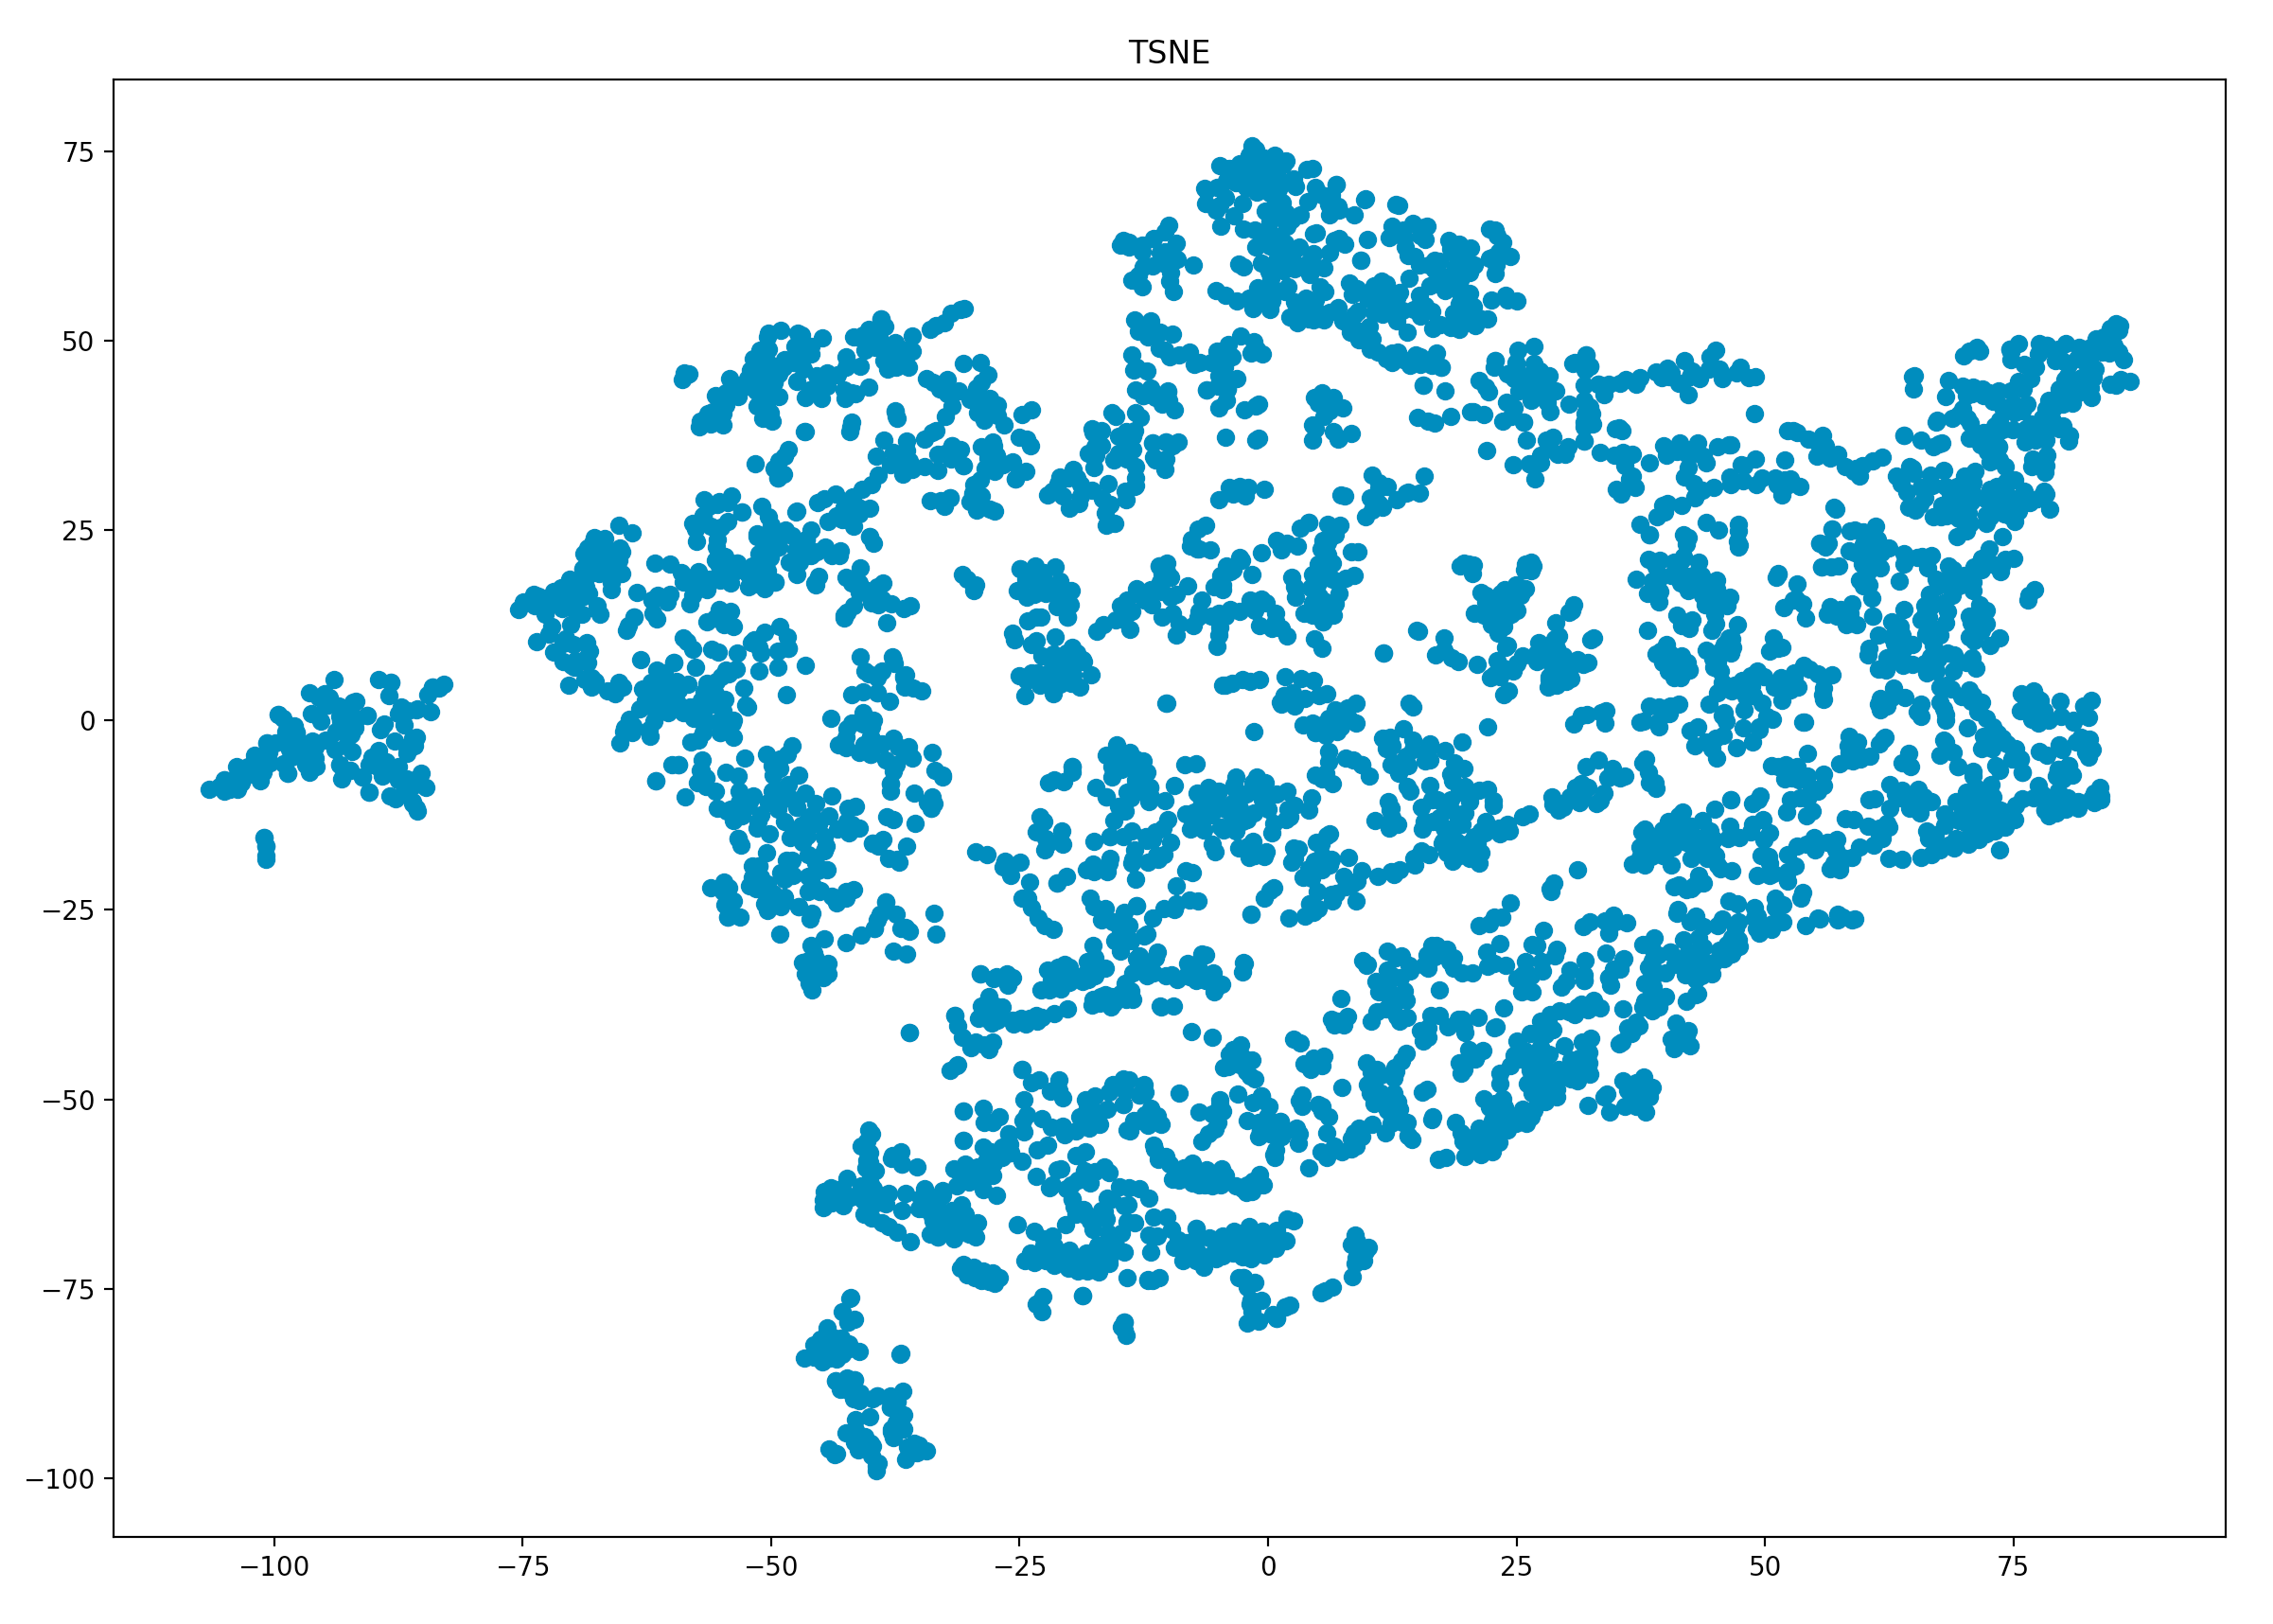
\includegraphics[width=0.9\textwidth]{./images/tsneParametersTest/learningRate/lr800-3hTSNE.png}
  % \caption{}
  % \label{figure:}
  \end{subfigure}%
  \begin{subfigure}{.5\textwidth}
    \centering
    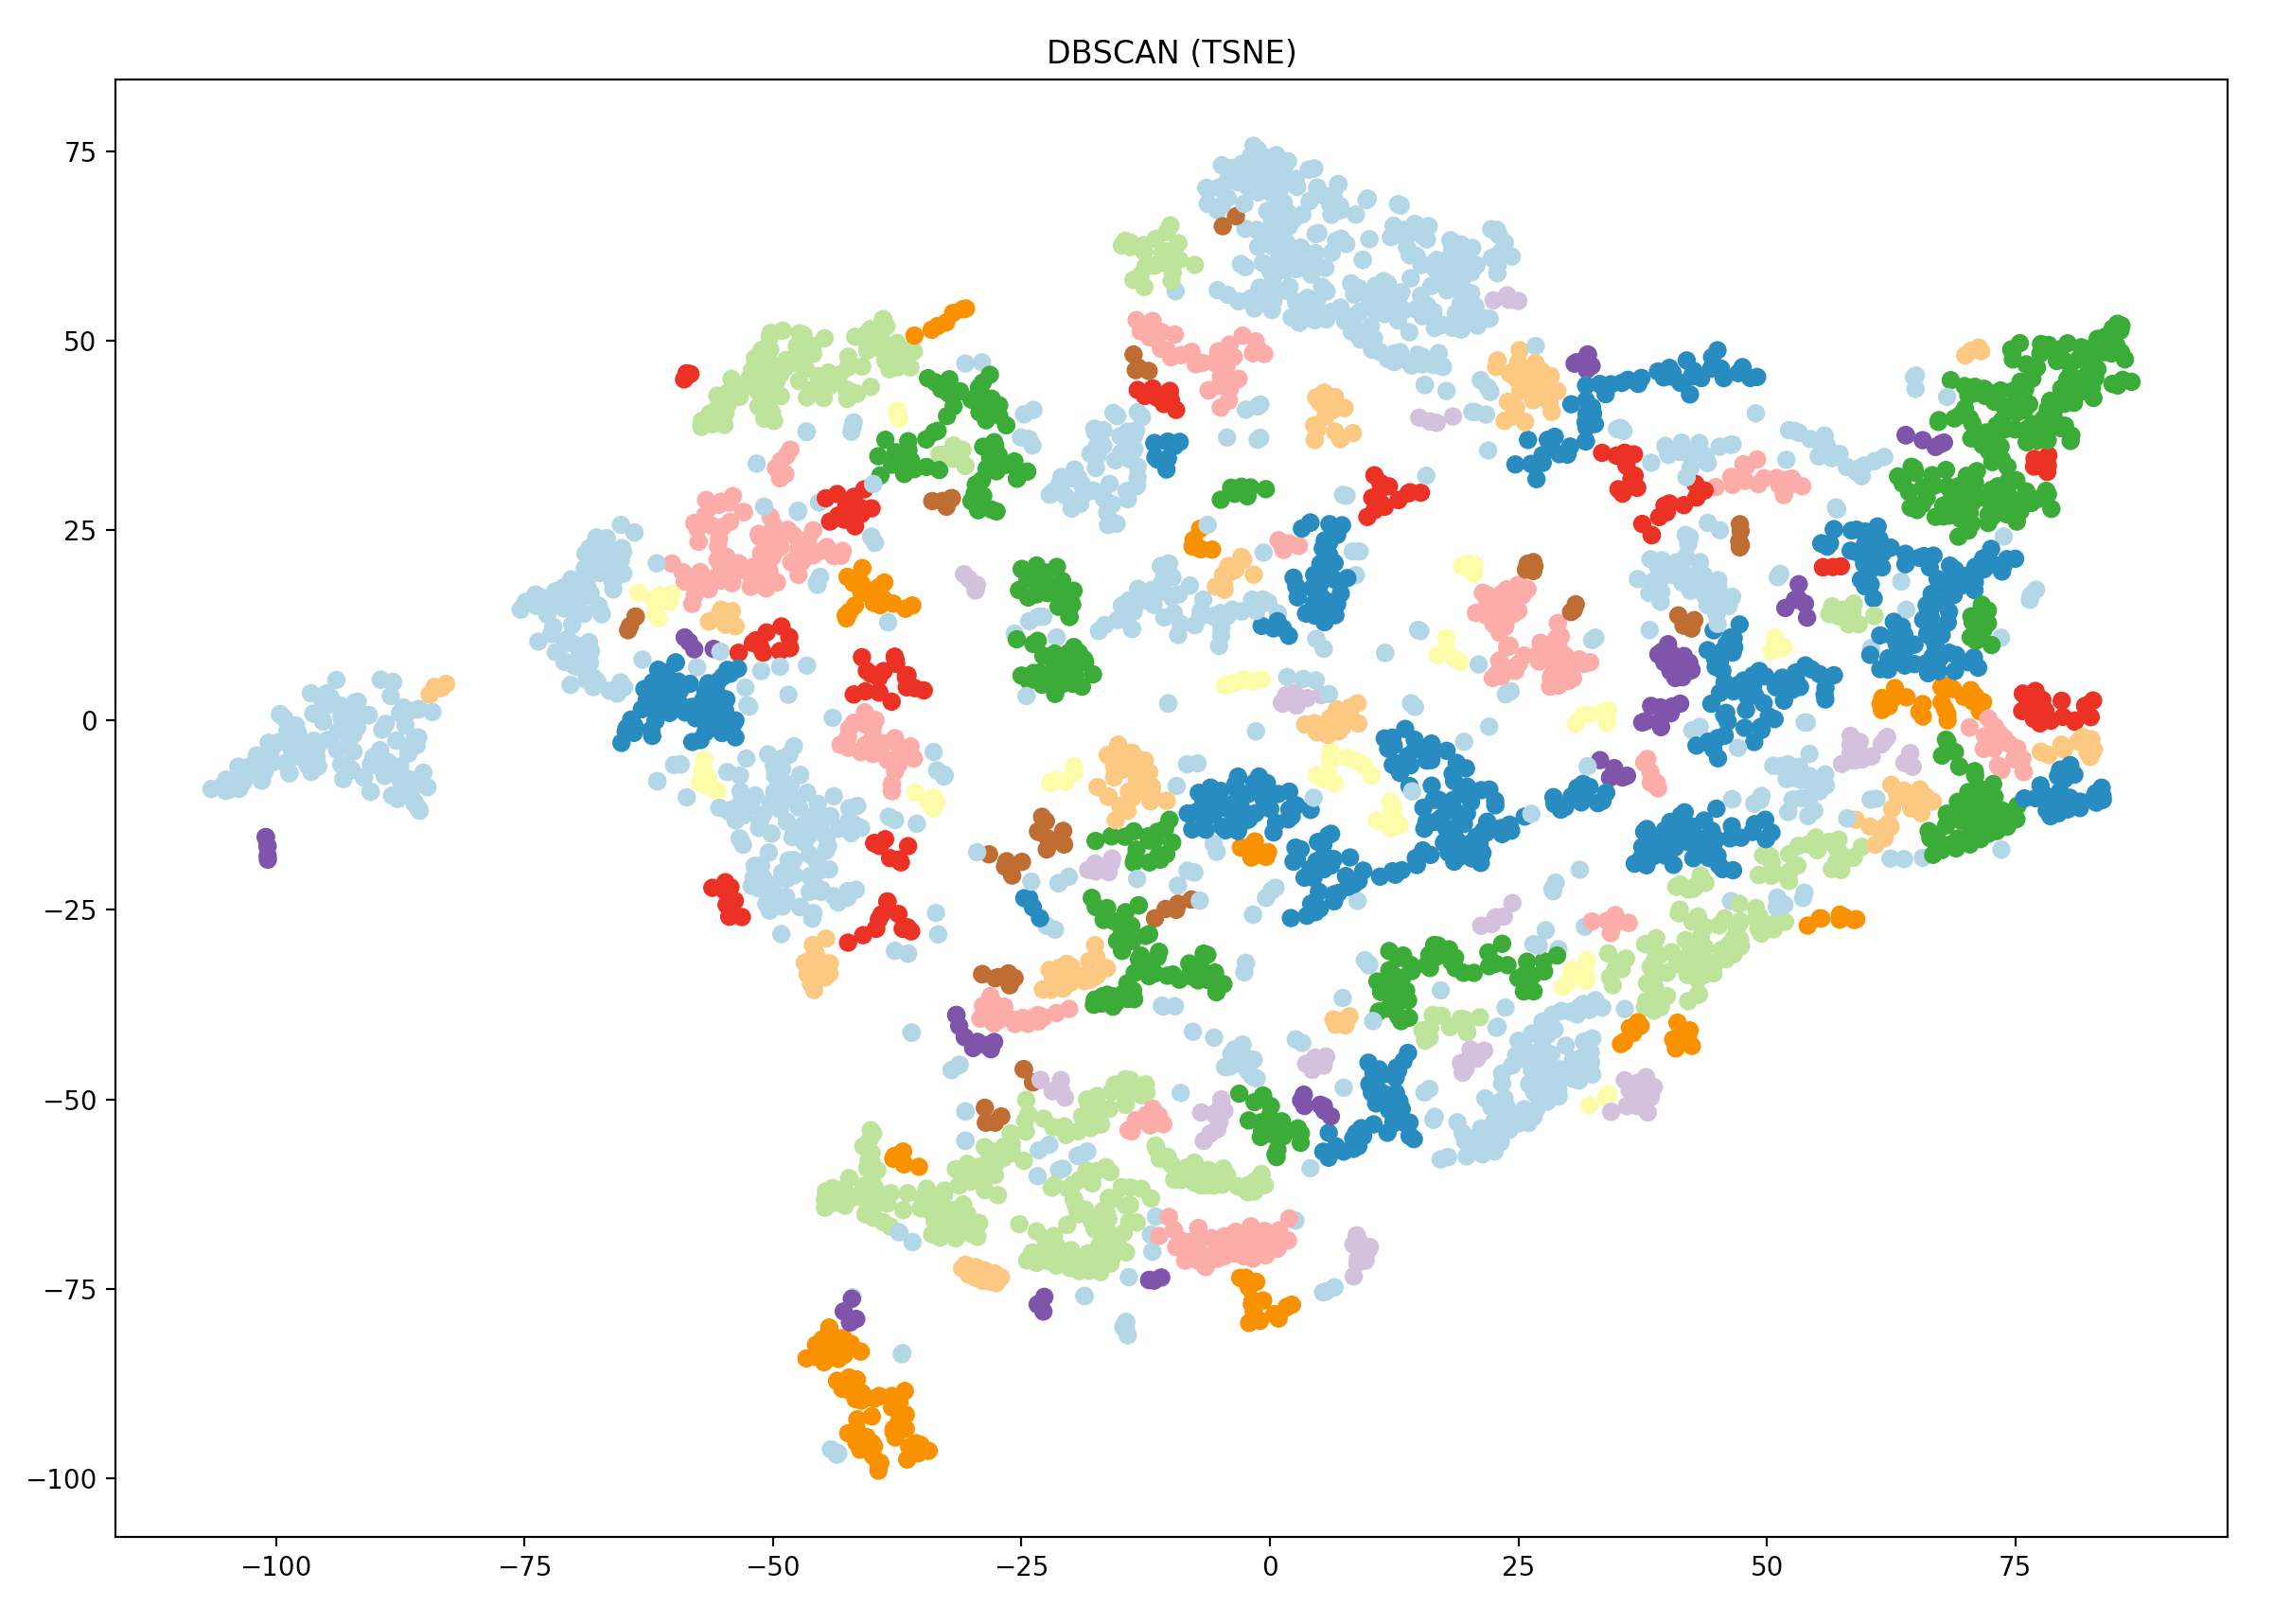
\includegraphics[width=0.9\textwidth]{./images/tsneParametersTest/learningRate/lr800-3hDBSCAN.png}
    % \caption{}
    % \label{figure:}
	\end{subfigure}
	\caption{\textbf{3h} data files, t-SNE calculated with the following parameters: perplexity=40, n\_iter=5000, \textbf{learning\_rate=800}}
  \label{figure:3hlr800TSNE}
\end{figure}


%------------------ LEARNING RATE 1000: ------------------
\subsubsection{Learning Rate = 1000}
% -- 1h, lr 1000 --
\begin{figure}[H]
  \centering
  \begin{subfigure}{.5\textwidth}
    \centering
    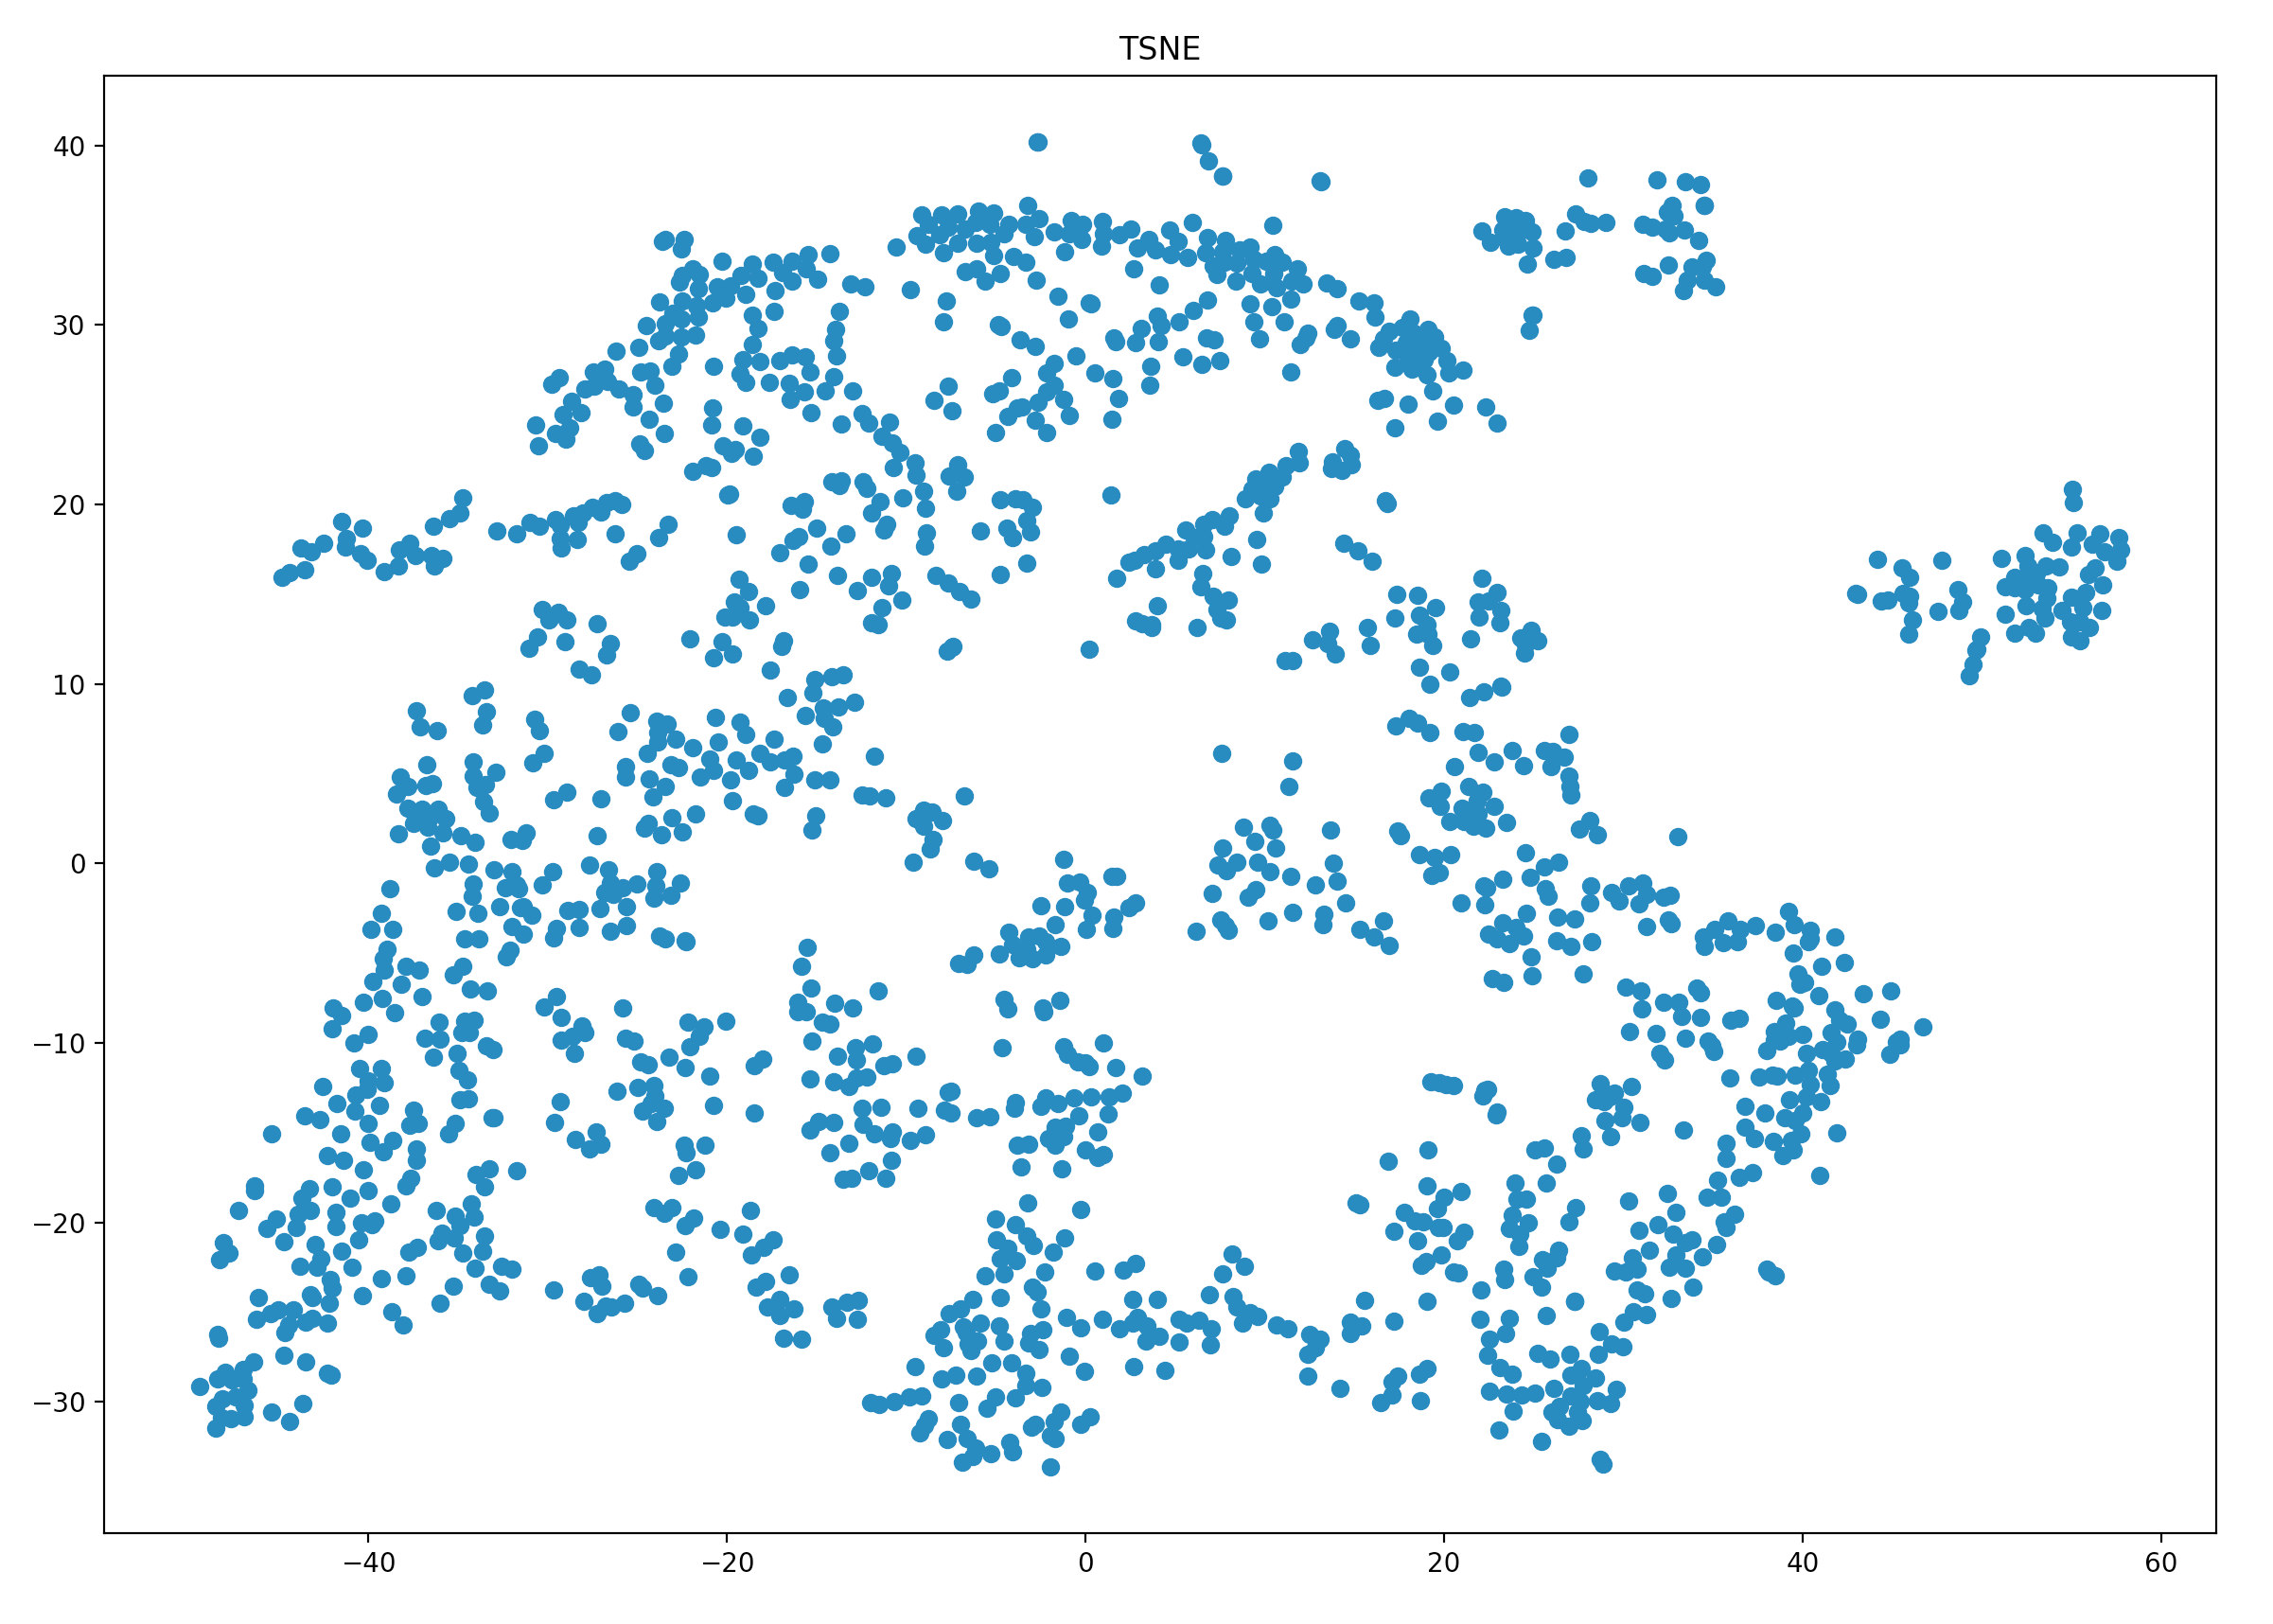
\includegraphics[width=0.9\textwidth]{./images/tsneParametersTest/learningRate/lr1000-1hTSNE.png}
  % \caption{}
  % \label{figure:}
  \end{subfigure}%
  \begin{subfigure}{.5\textwidth}
    \centering
    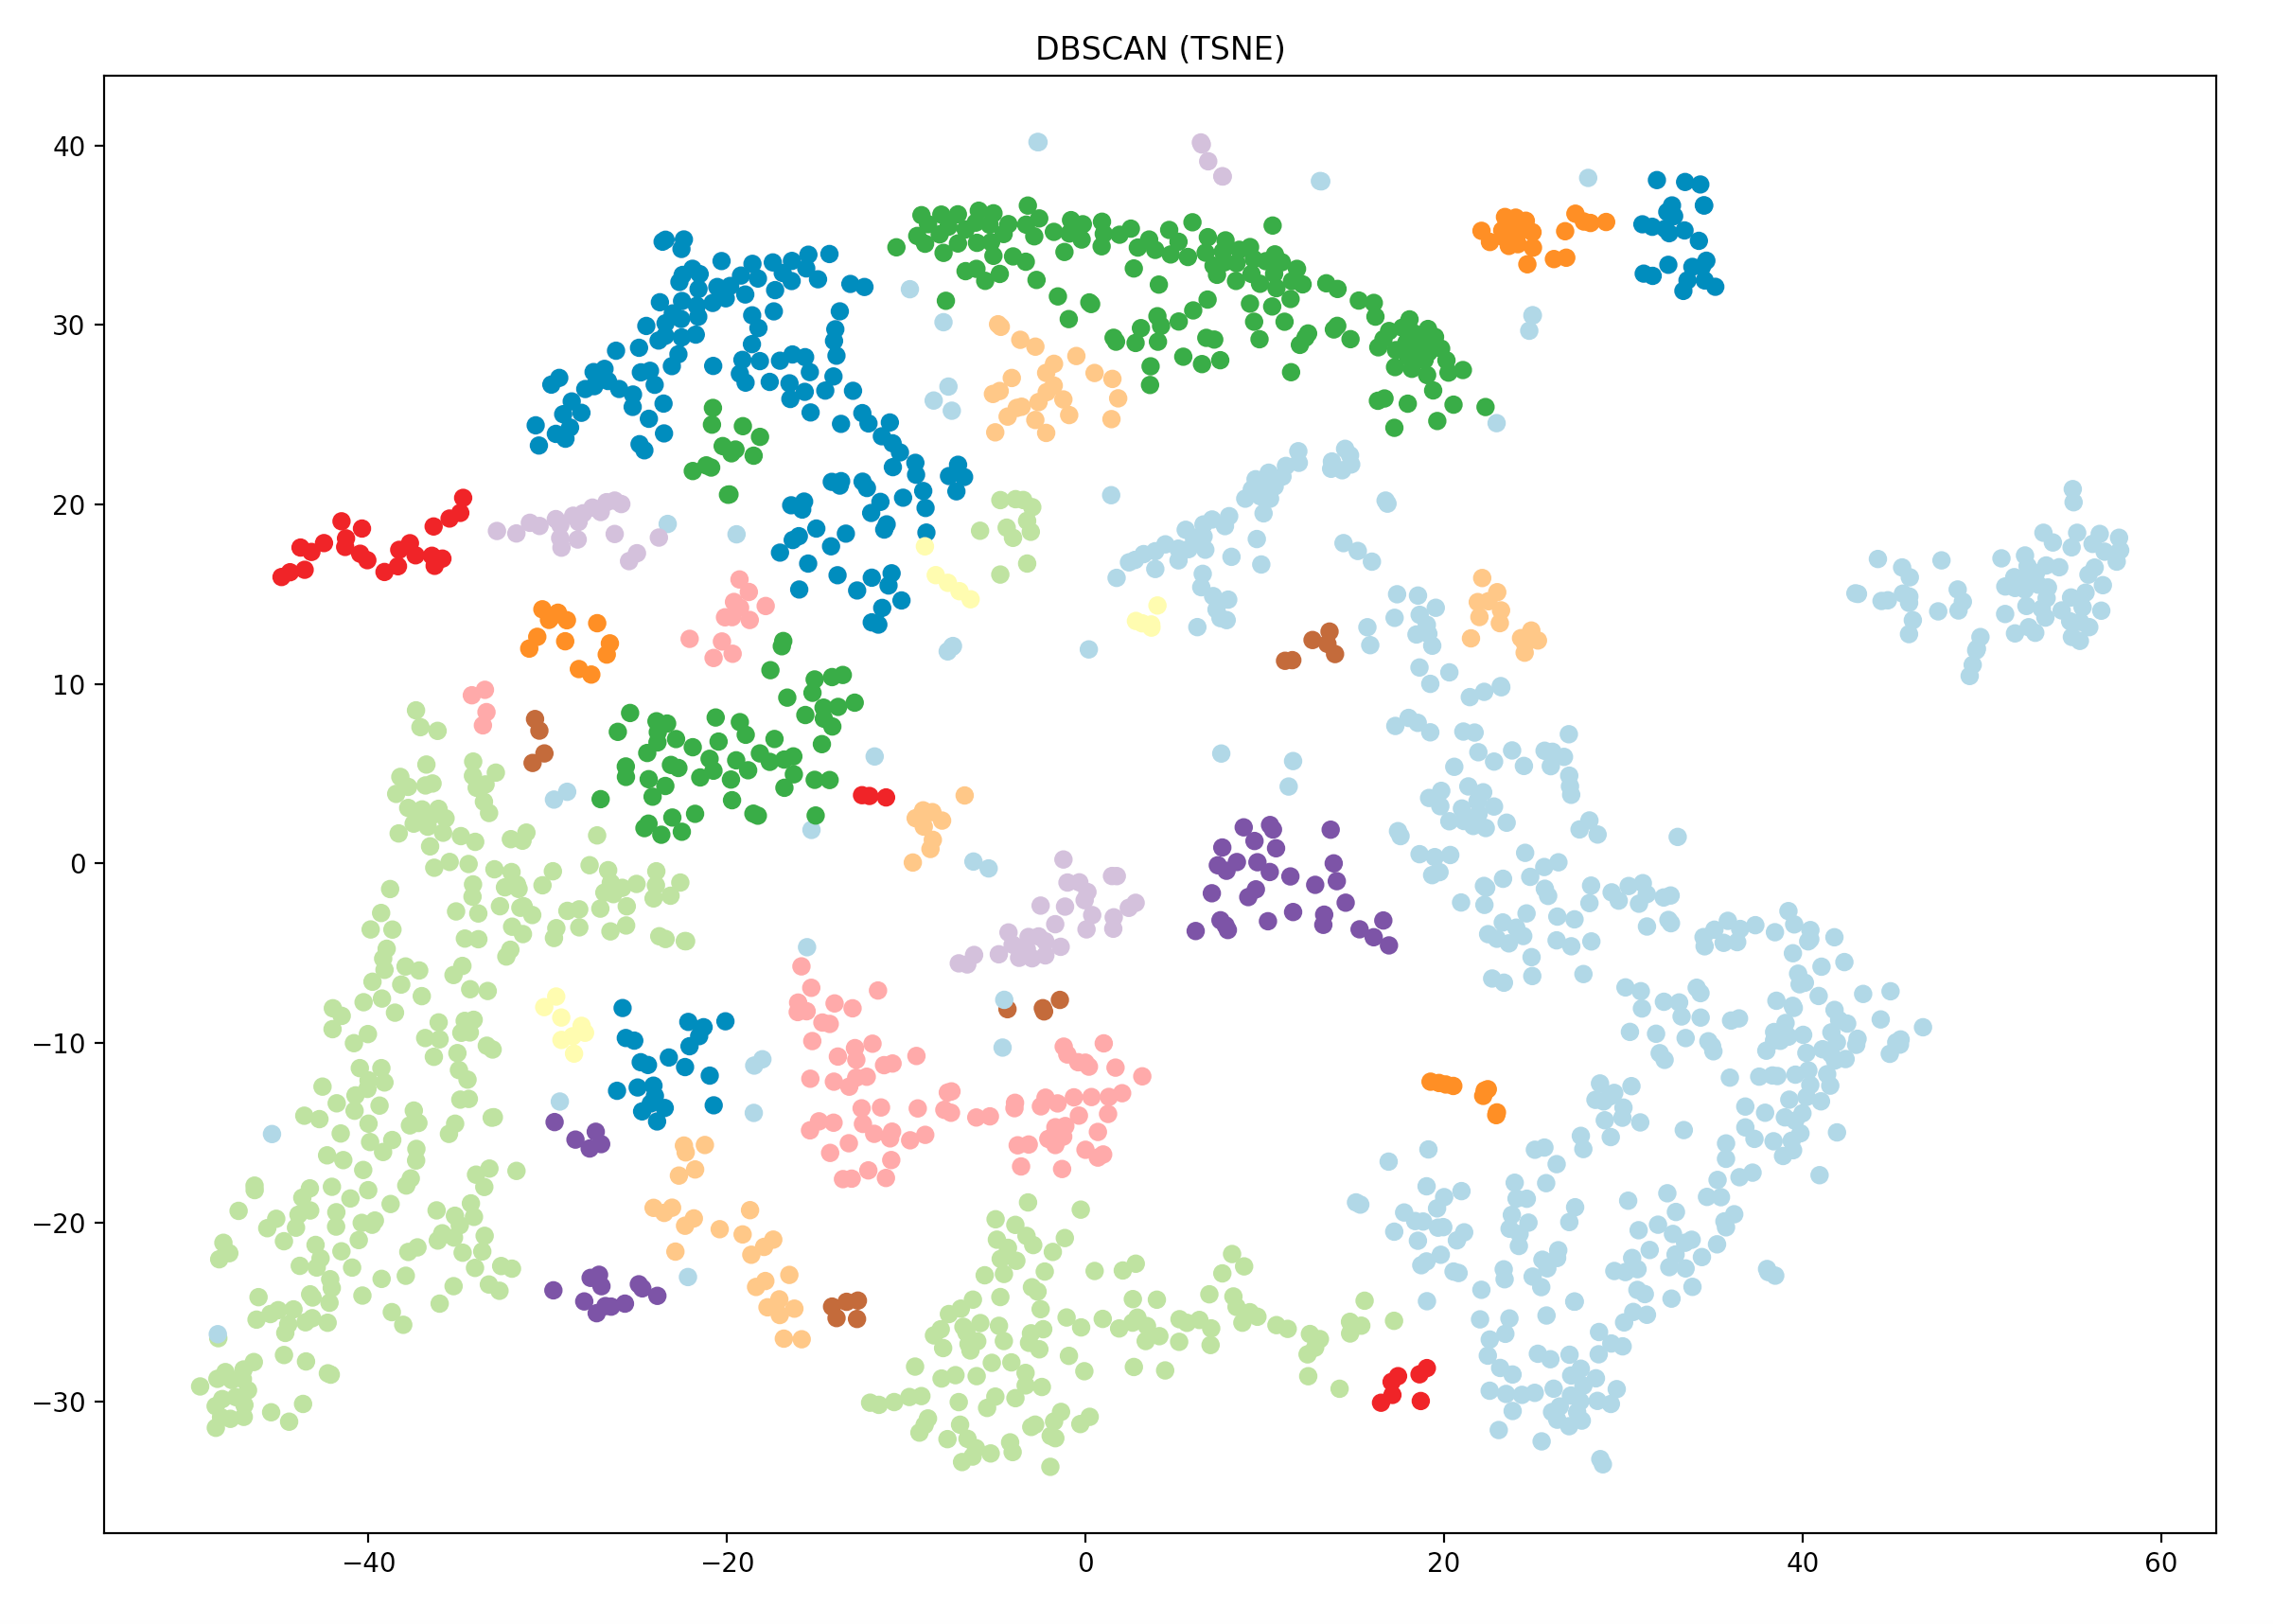
\includegraphics[width=0.9\textwidth]{./images/tsneParametersTest/learningRate/lr1000-1hDBSCAN.png}
    % \caption{}
    % \label{figure:}
  \end{subfigure}
	\caption{\textbf{1h} data files, t-SNE calculated with the following parameters: perplexity=40, n\_iter=5000, \textbf{learning\_rate=1000}}
	\label{figure:1hlr1000TSNE}
\end{figure}

% -- 3h, lr 1000 --
\begin{figure}[H]
	\centering
	
  \centering
	\begin{subfigure}{.5\textwidth}
    \centering
    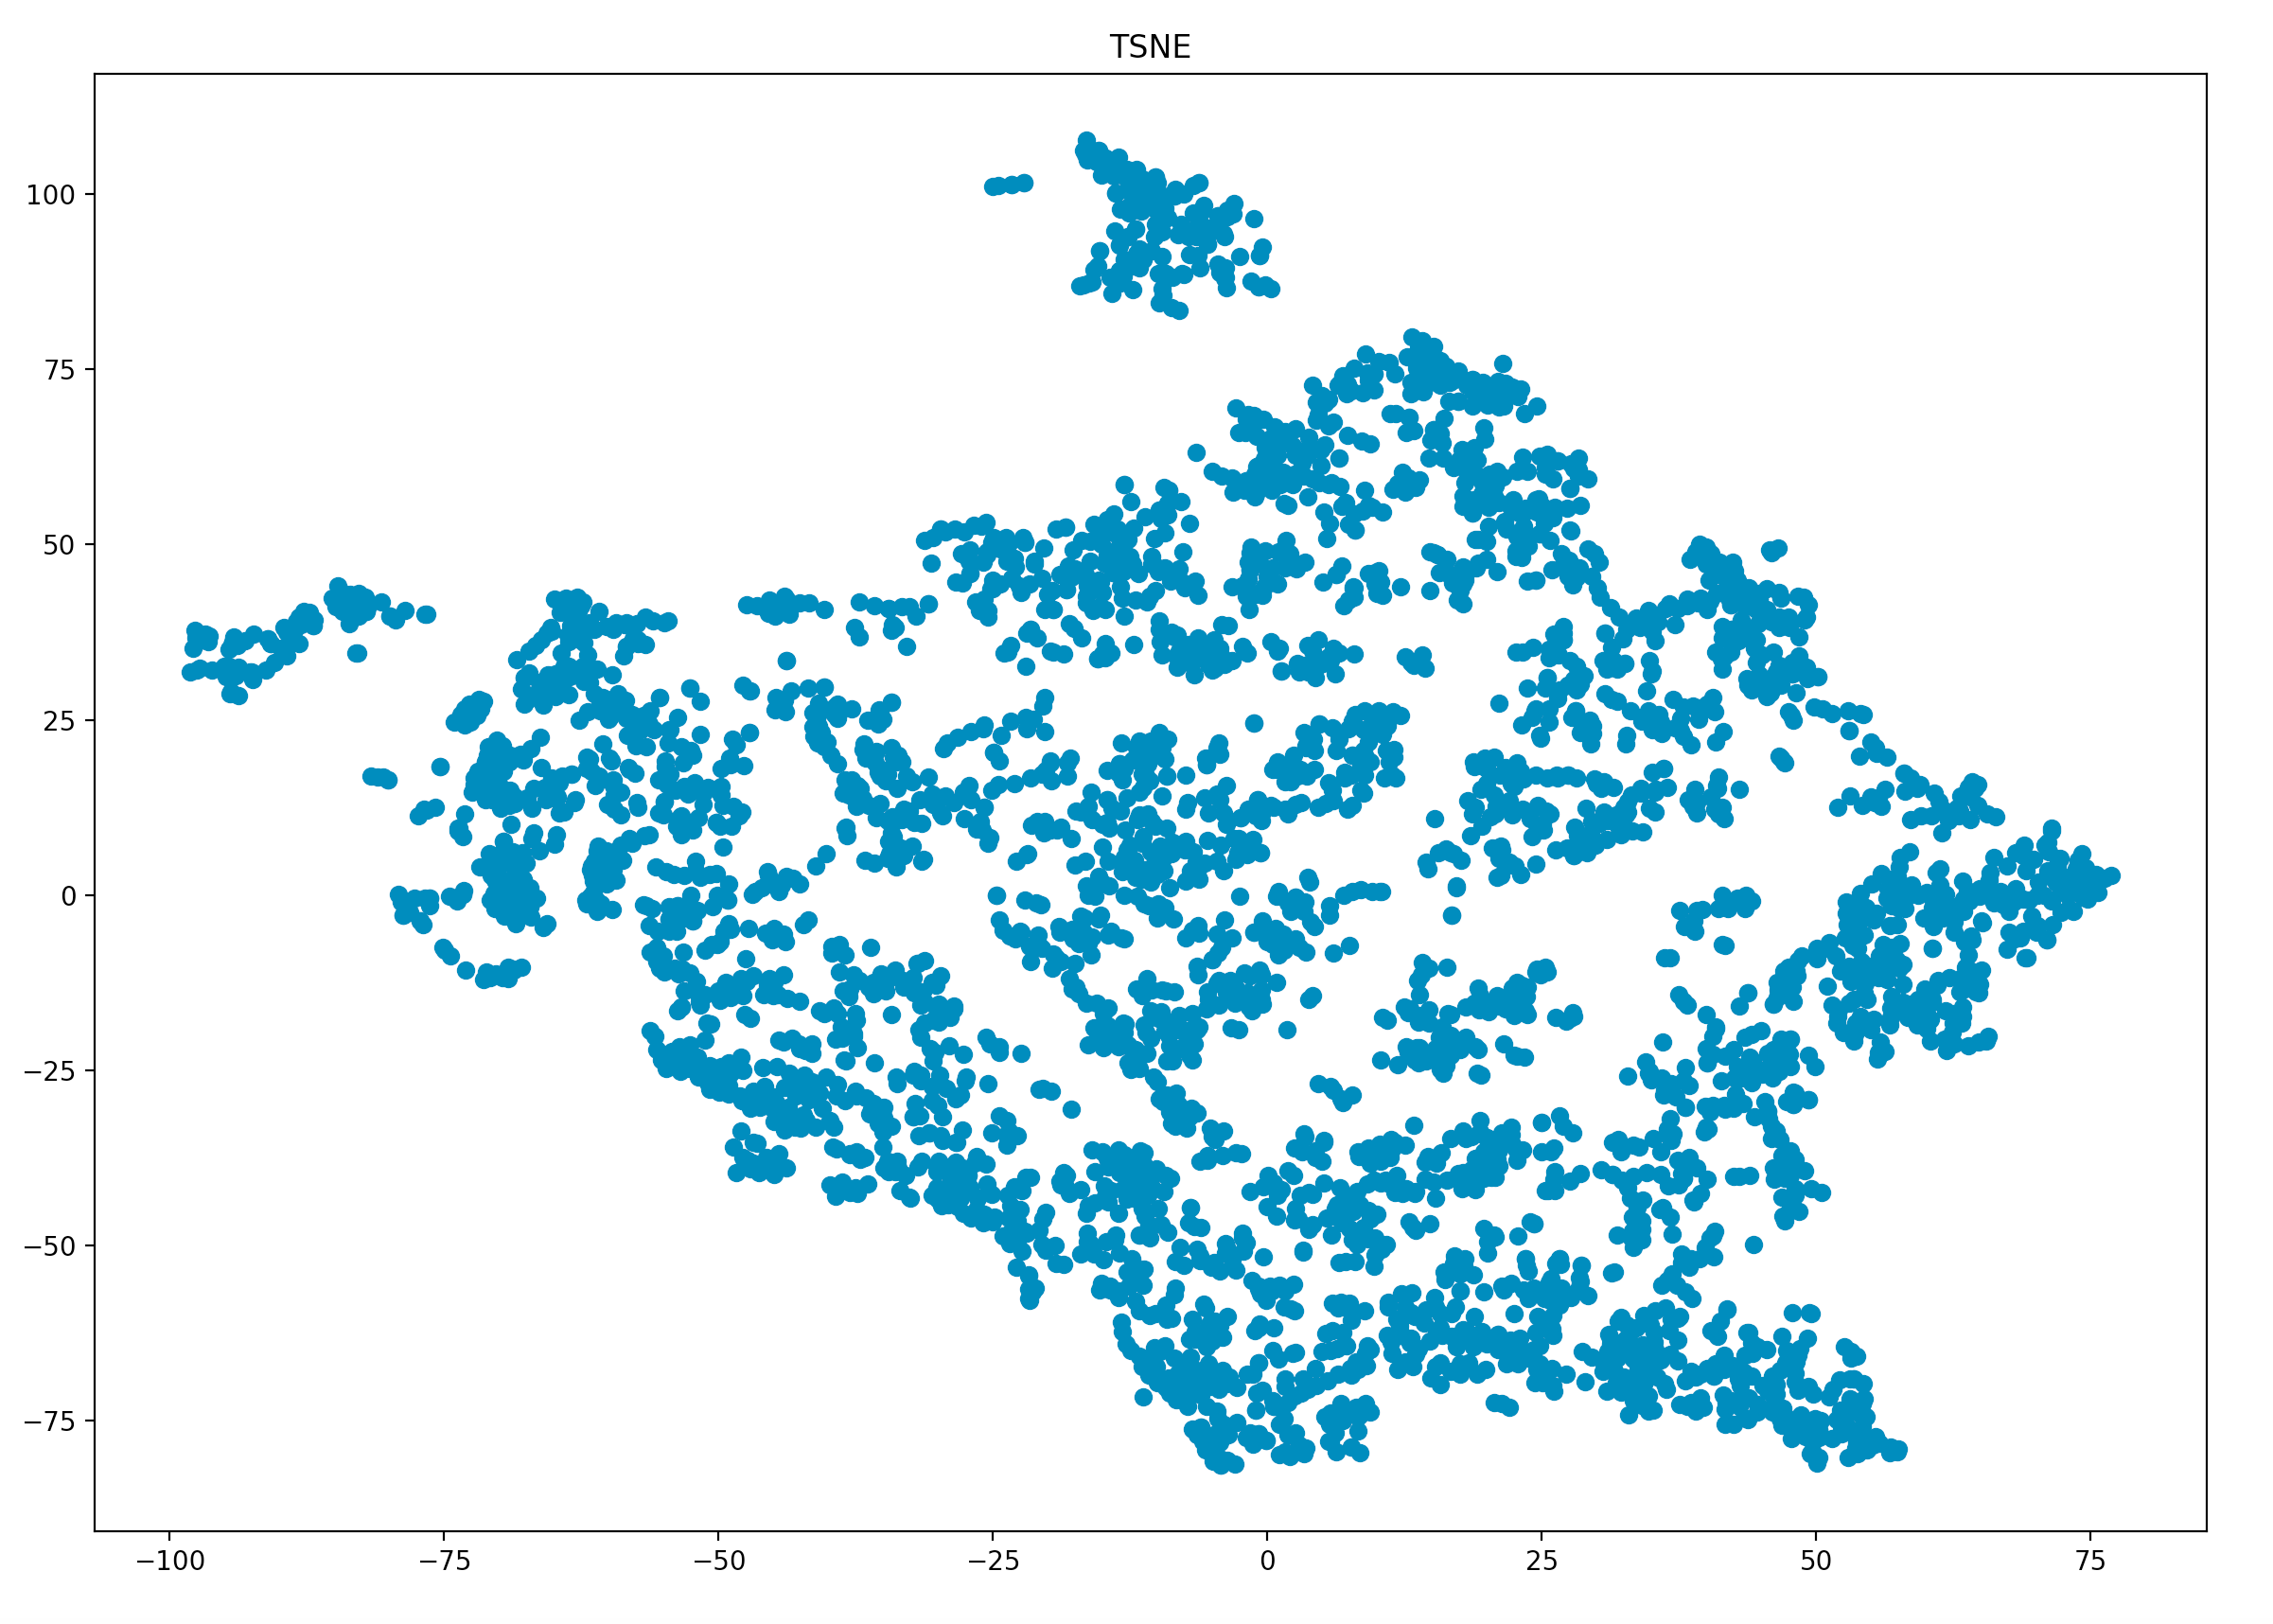
\includegraphics[width=0.9\textwidth]{./images/tsneParametersTest/learningRate/lr1000-3hTSNE.png}
  % \caption{}
  % \label{figure:}
  \end{subfigure}%
  \begin{subfigure}{.5\textwidth}
    \centering
    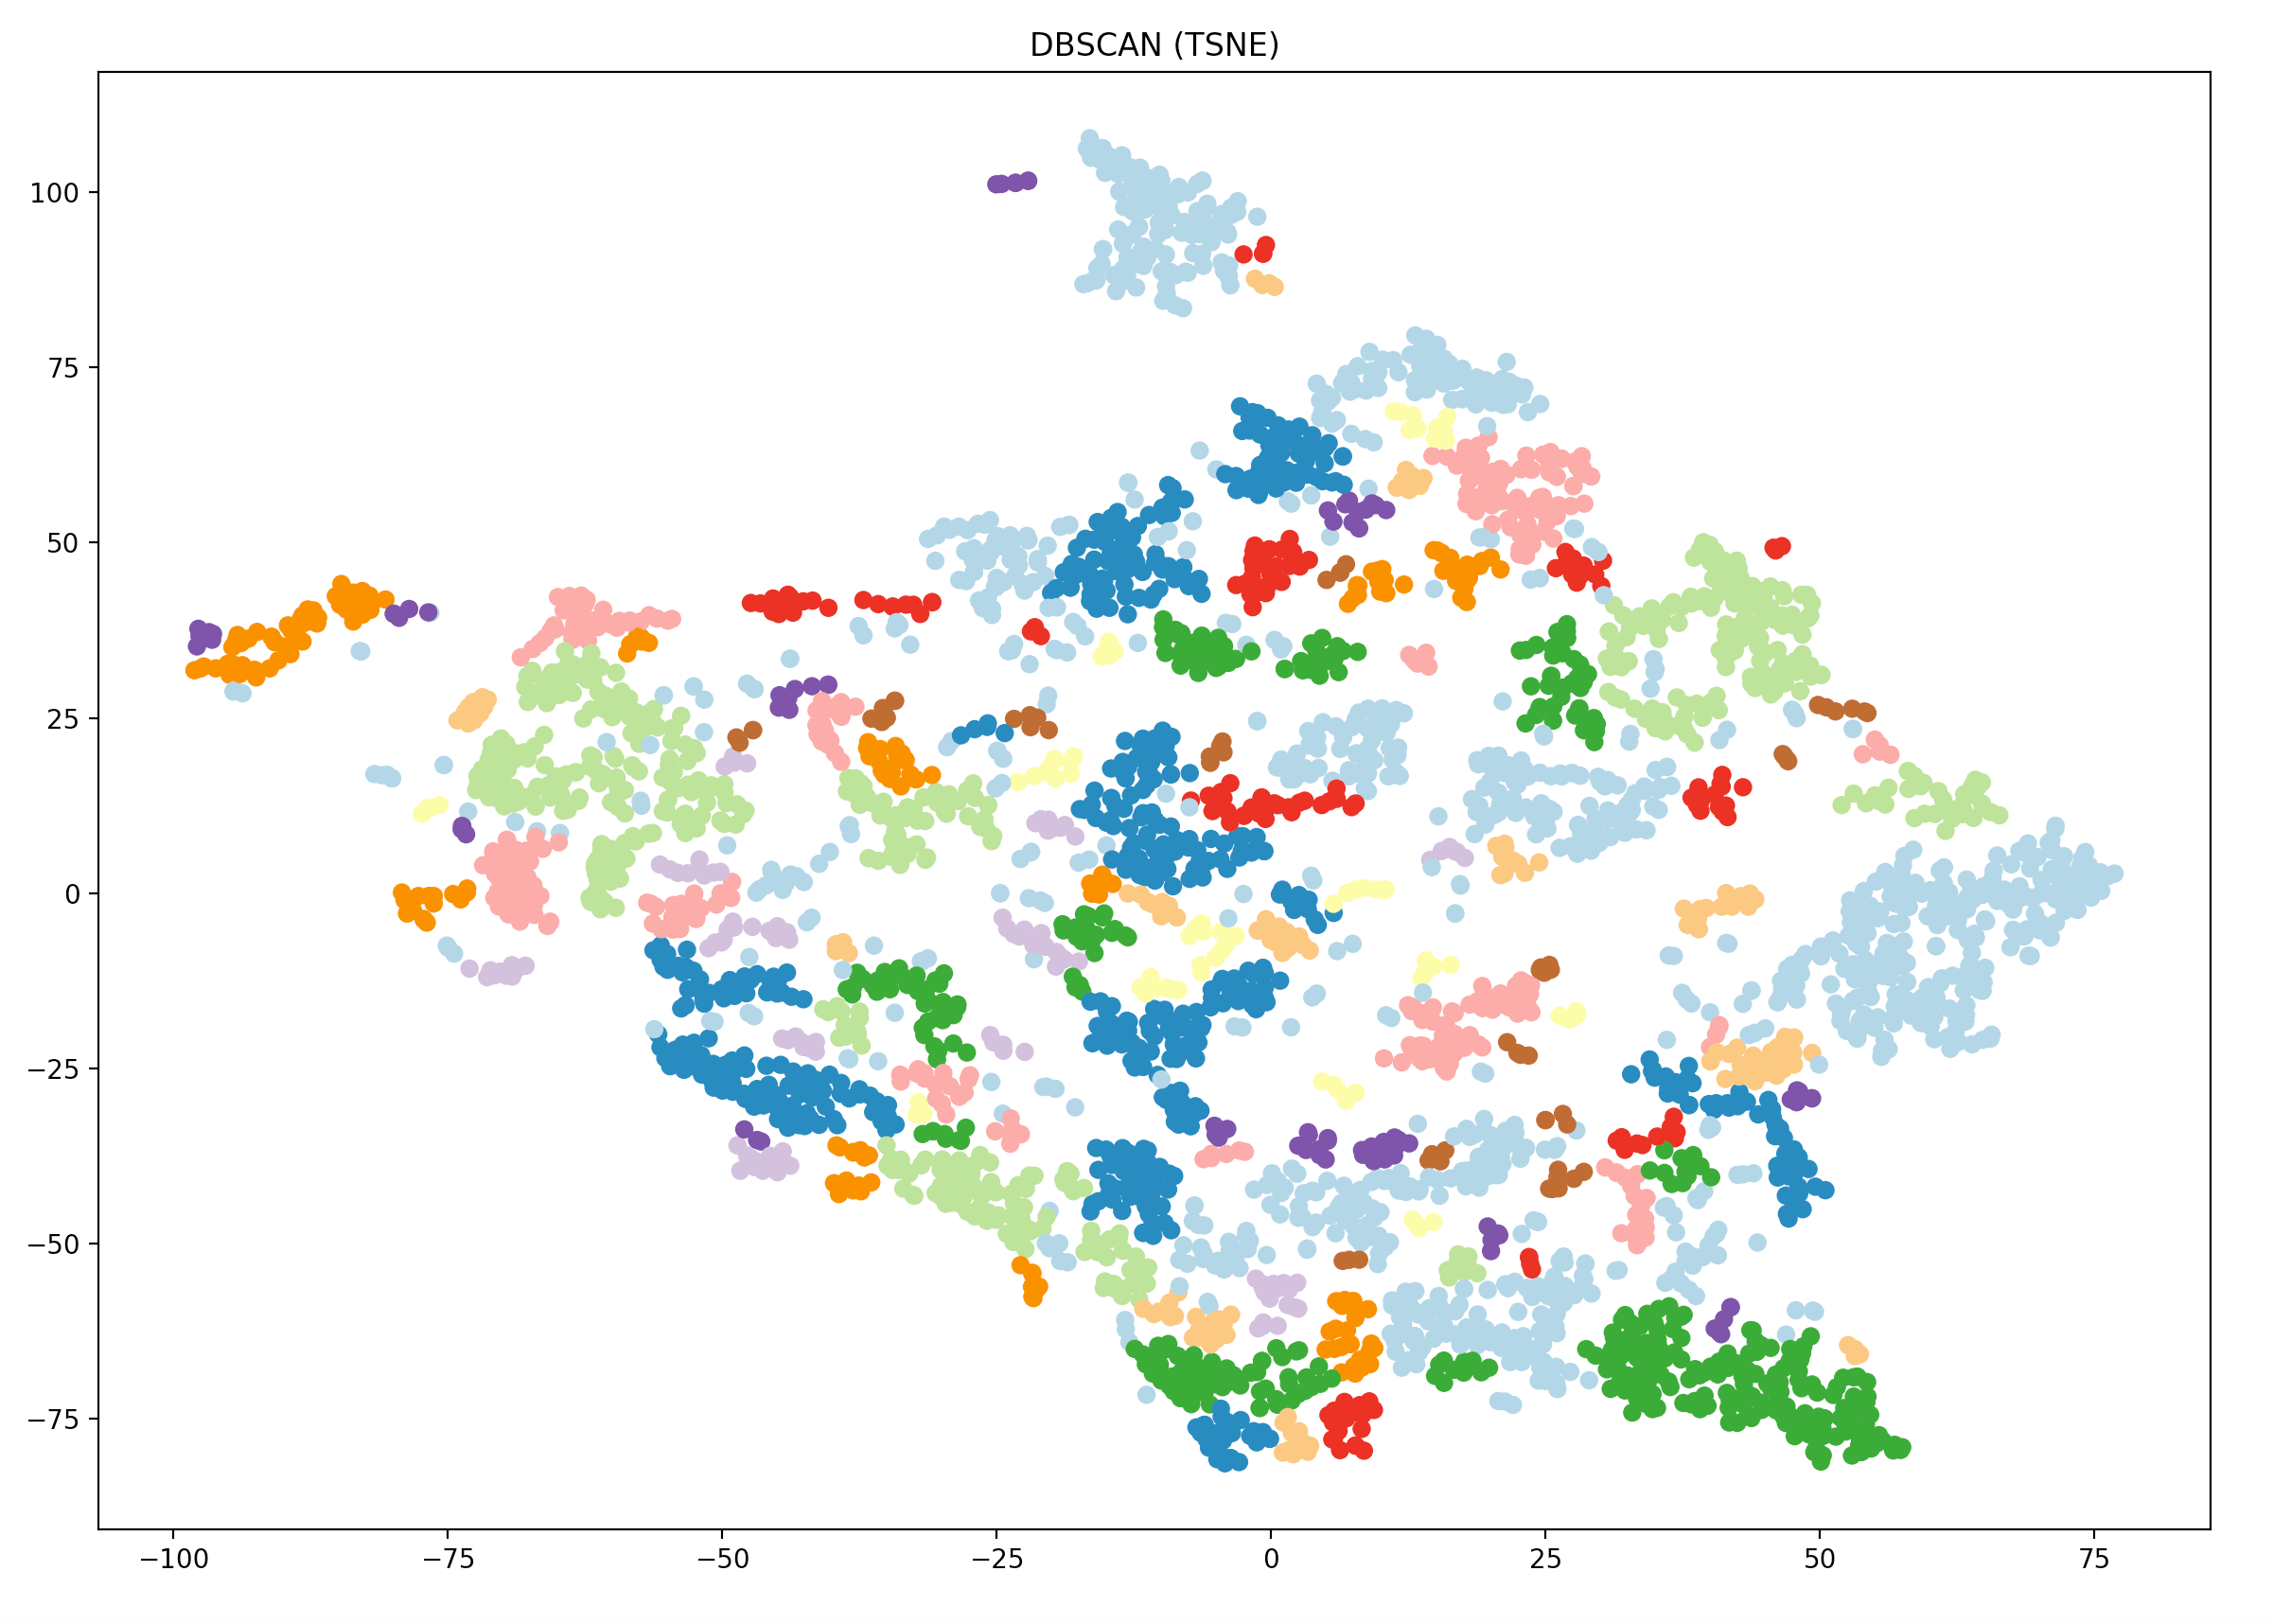
\includegraphics[width=0.9\textwidth]{./images/tsneParametersTest/learningRate/lr1000-3hDBSCAN.png}
    % \caption{}
    % \label{figure:}
	\end{subfigure}
	\caption{\textbf{3h} data files, t-SNE calculated with the following parameters: perplexity=40, n\_iter=5000, \textbf{learning\_rate=1000}}
  \label{figure:3hlr1000TSNE}
\end{figure}



\subsubsection{Learning Rate Detailed Comparison Results }
\label{appendix:comparelearningRateDetailed}

\begin{figure}
  \centering
  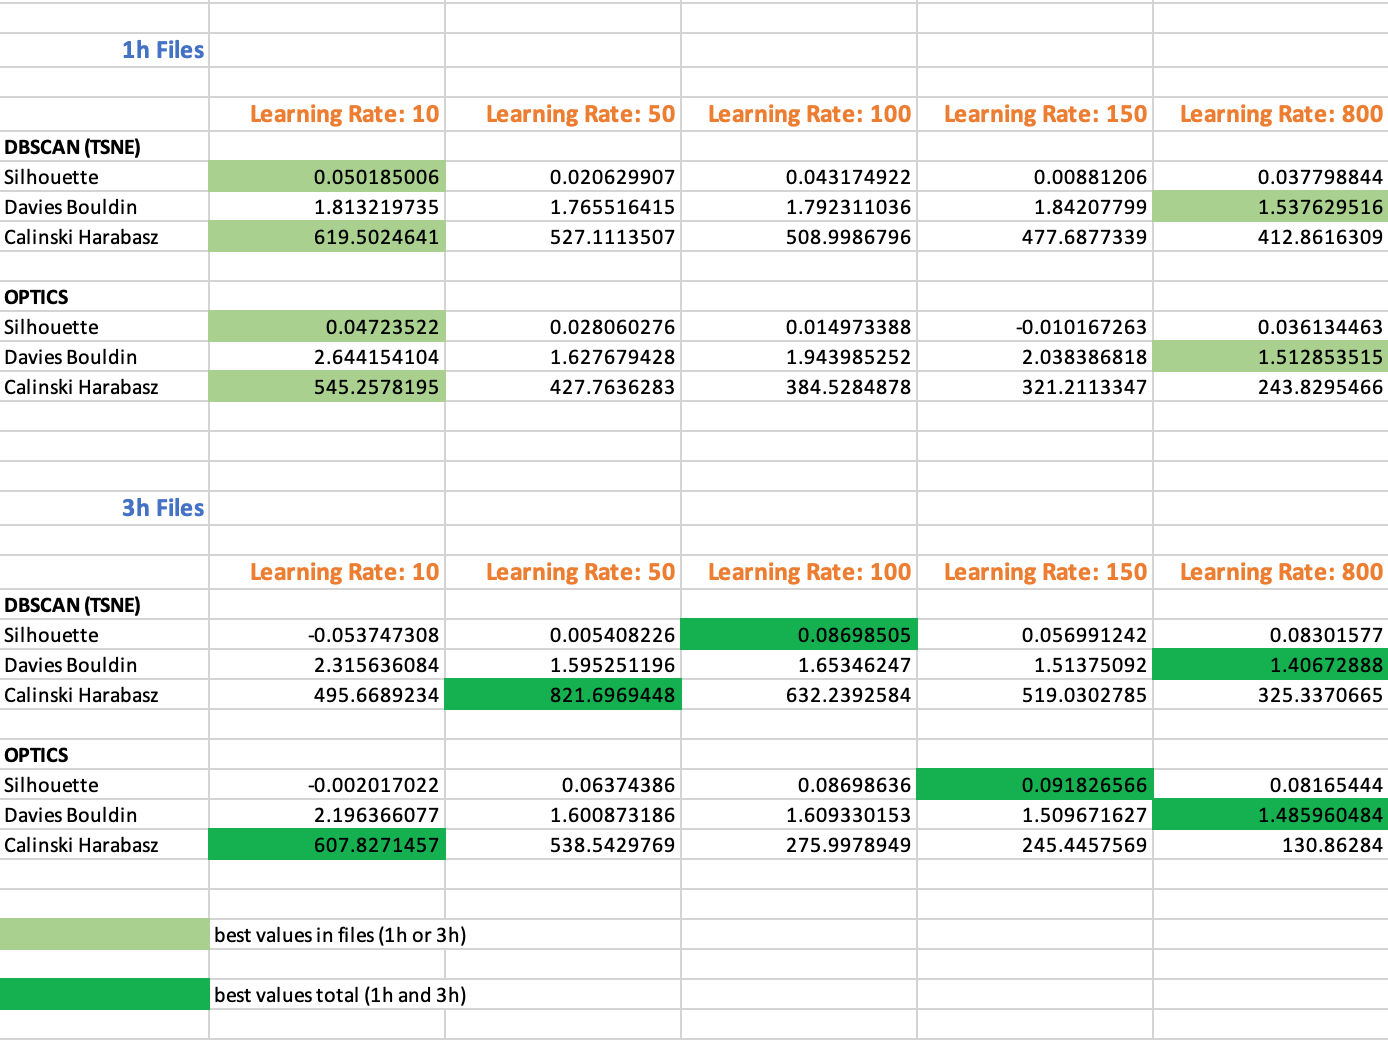
\includegraphics[width=0.8\textwidth]{./images/tsneParametersTest/learningRate/learningRateEvaluationScoresDetailed.png}
  \caption{Comparison of Silhouette Coefficient, Davies-Bouldin Index, and Caliński-Harabasz Index for different t-SNE \textbf{learning rate} values. The lighter green highlighted values indicate the best values of that file aggregation (1h or 3h files). The dark green highlighted values illustrate the overall best values over all files (1h and 3h files).}
  \label{figure:learningRateEvaluationScoresDetailed}
\end{figure}

\begin{figure}
  \centering
  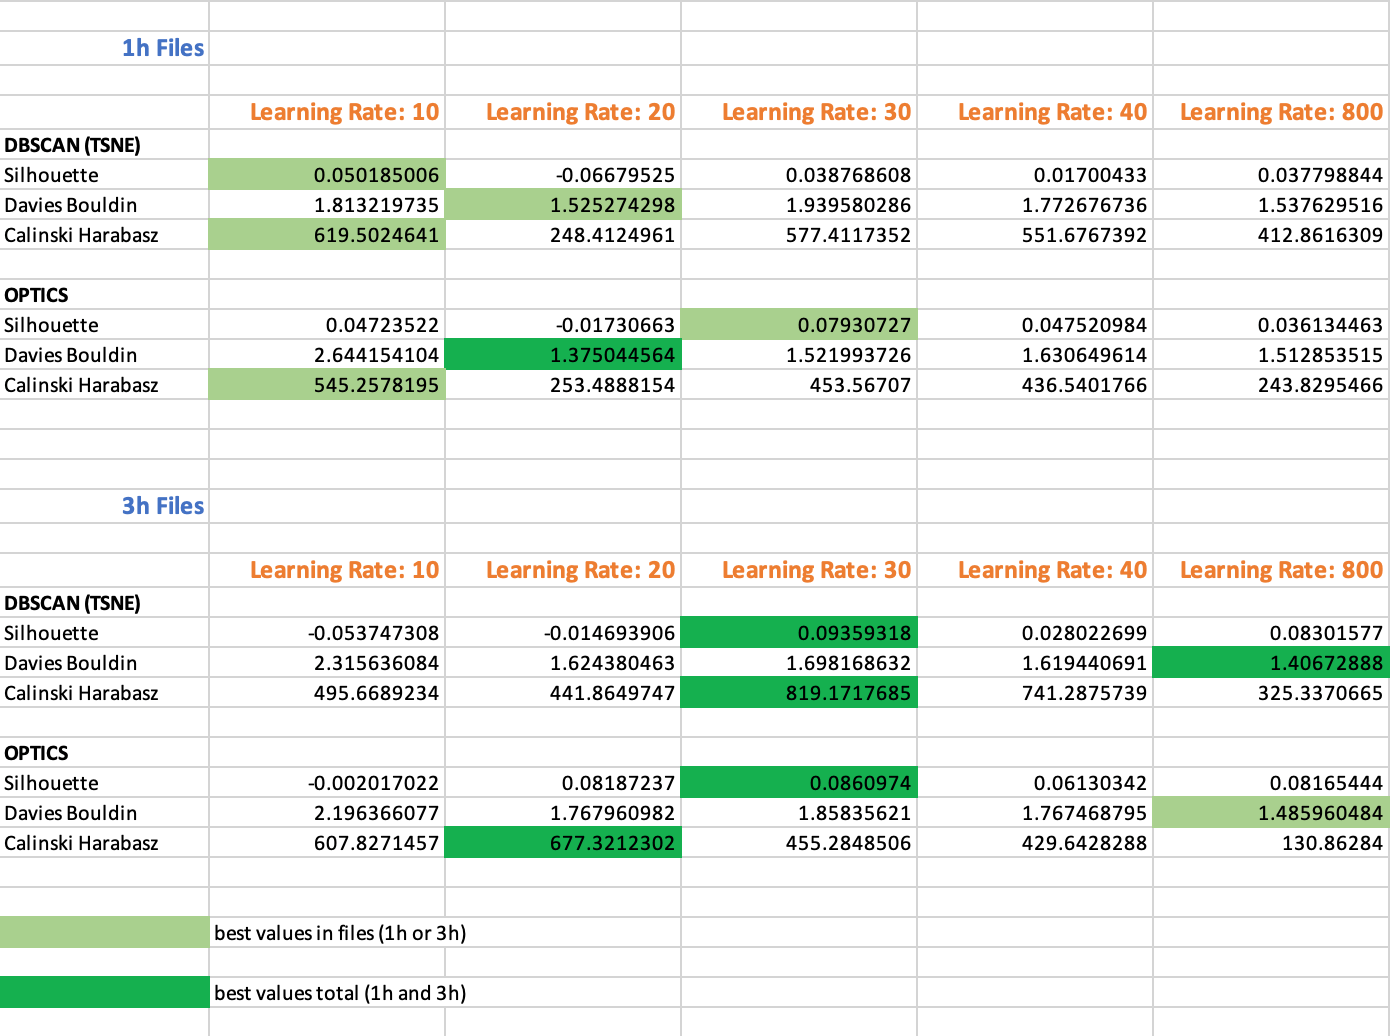
\includegraphics[width=0.8\textwidth]{./images/tsneParametersTest/learningRate/learningRateEvaluationScoresDetailed2.png}
  \caption{Comparison of Silhouette Coefficient, Davies-Bouldin Index, and Caliński-Harabasz Index for different t-SNE \textbf{learning rate} values. The lighter green highlighted values indicate the best values of that file aggregation (1h or 3h files). The dark green highlighted values illustrate the overall best values over all files (1h and 3h files).}
  \label{figure:learningRateEvaluationScoresDetailed2}
\end{figure}

%.................................COMPARISON AVERAGES..................................
\subsubsection{Learning Rate Comparison Results (Average of two different t-SNE runs)}
\label{appendix:compareAverageLearningRate}


\begin{figure}[H]
  \centering
  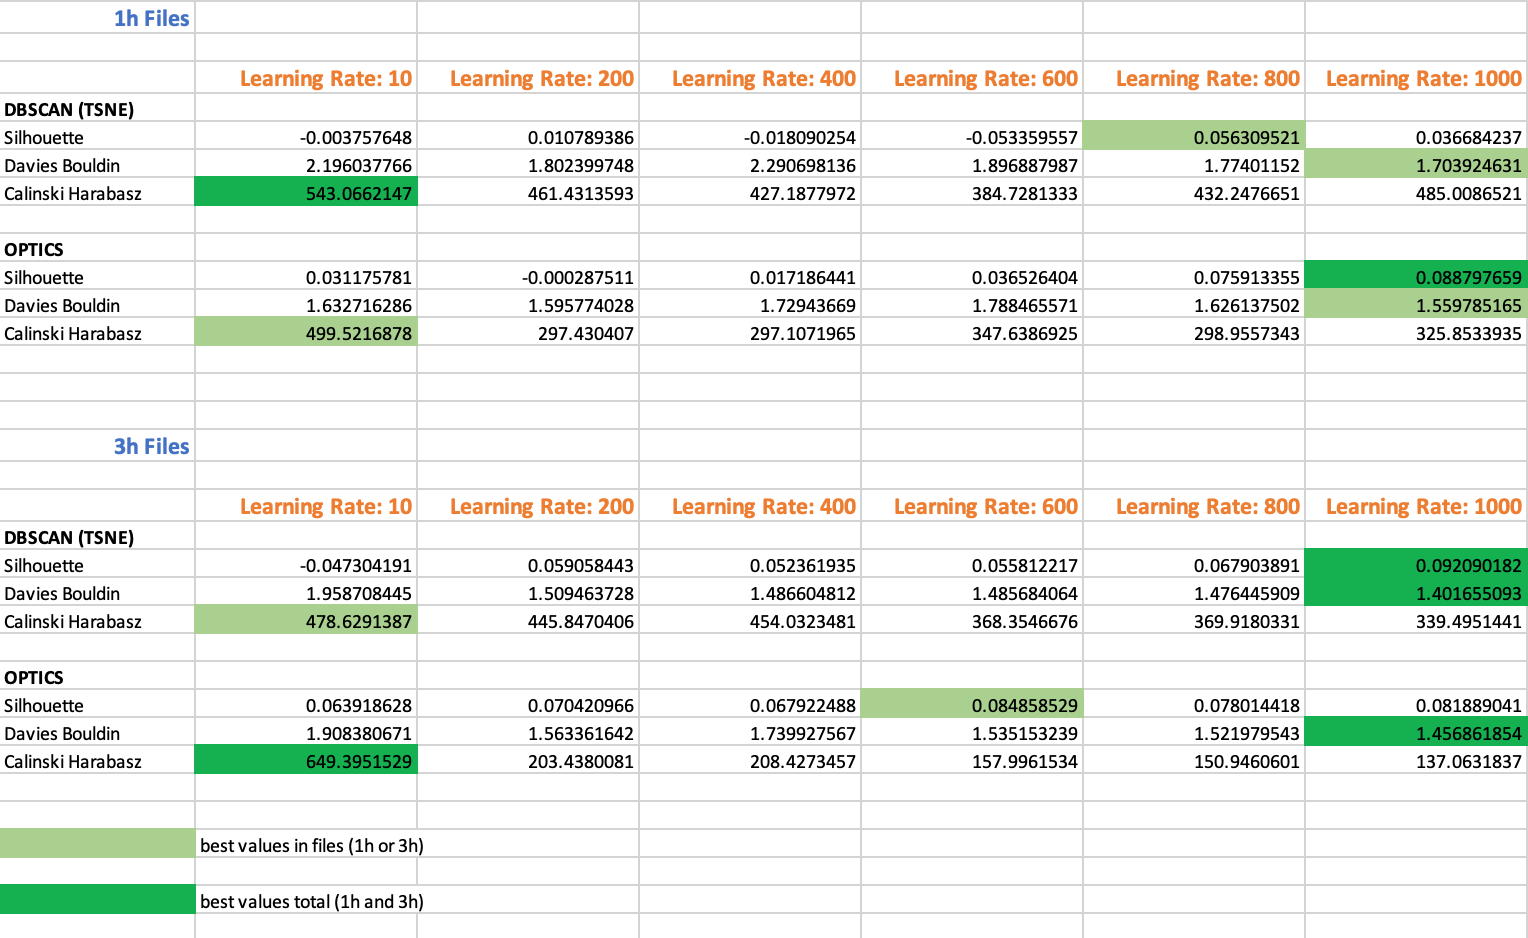
\includegraphics[width=0.8\textwidth]{./images/tsneParametersTest/learningRate/learningRateEvaluationScoresAverage.png}
  \caption{Comparison of Silhouette Coefficient, Davies-Bouldin Index, and Caliński-Harabasz Index for different t-SNE \textbf{learning rate} values. The lighter green highlighted values indicate the best values of that file aggregation (1h or 3h files). The dark green highlighted values illustrate the overall best values over all files (1h and 3h files).}
  \label{figure:learningRateEvaluationScoresAverage}
\end{figure}

\begin{figure}[H]
  \centering
  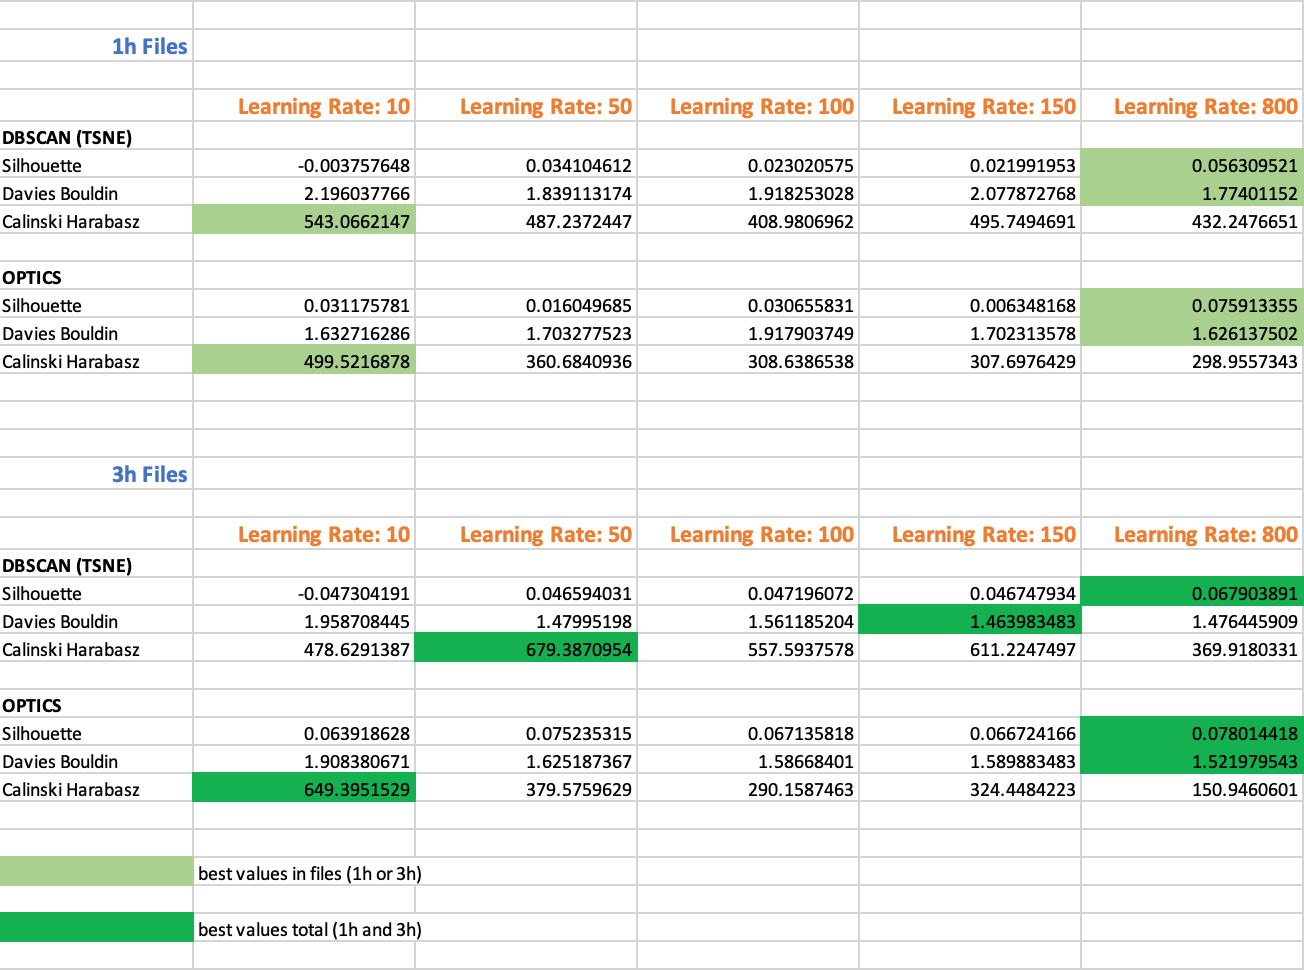
\includegraphics[width=0.8\textwidth]{./images/tsneParametersTest/learningRate/learningRateEvaluationScoresAverageDetailed.png}
  \caption{Comparison of Silhouette Coefficient, Davies-Bouldin Index, and Caliński-Harabasz Index for different t-SNE \textbf{learning rate} values. The lighter green highlighted values indicate the best values of that file aggregation (1h or 3h files). The dark green highlighted values illustrate the overall best values over all files (1h and 3h files).}
  \label{figure:learningRateEvaluationScoresAverageDetailed}
\end{figure}

\begin{figure}[H]
  \centering
  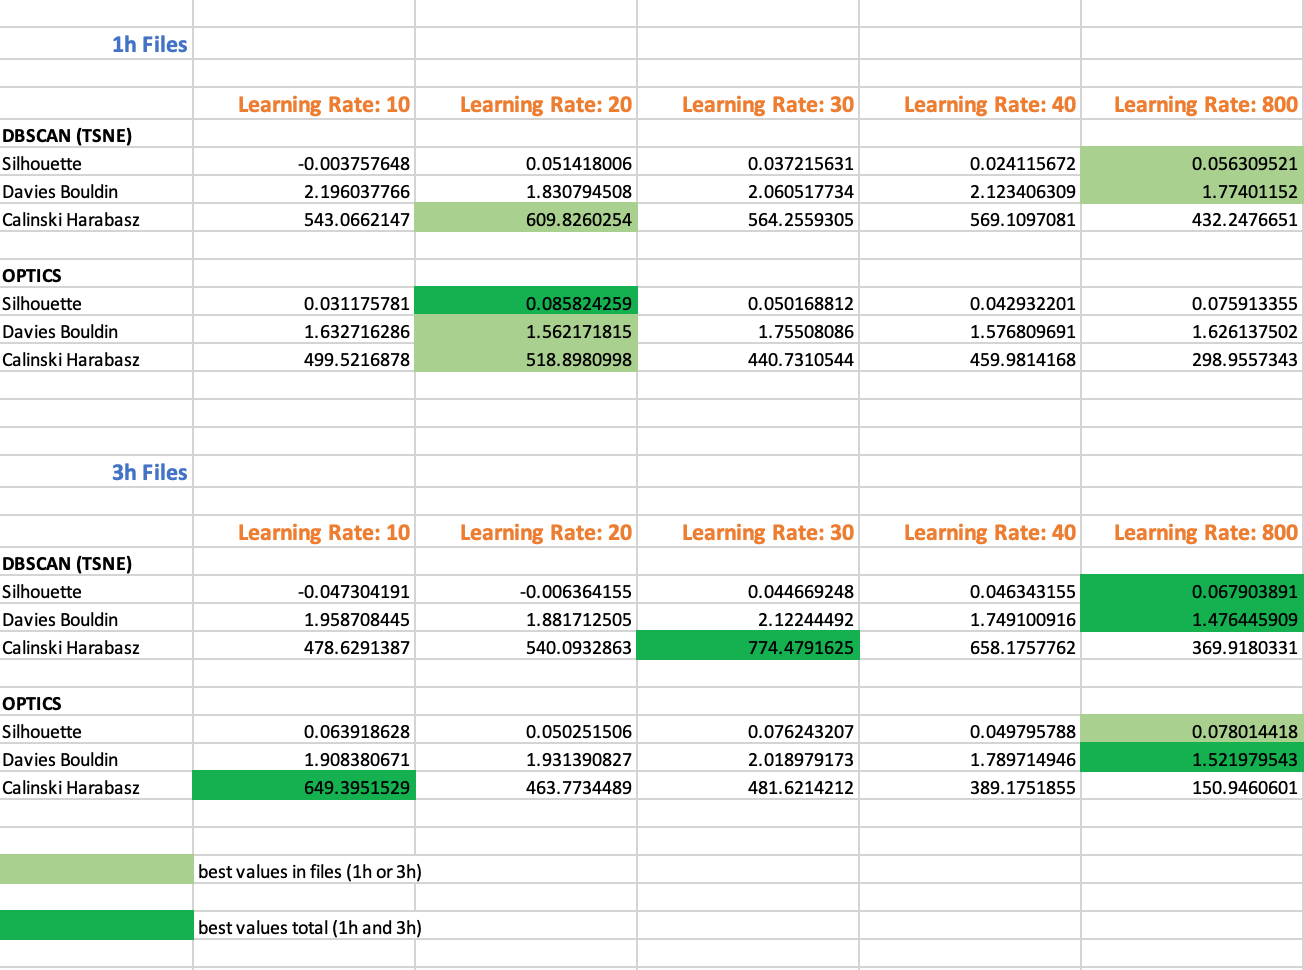
\includegraphics[width=0.8\textwidth]{./images/tsneParametersTest/learningRate/learningRateEvaluationScoresAverageDetailed2.png}
  \caption{Comparison of Silhouette Coefficient, Davies-Bouldin Index, and Caliński-Harabasz Index for different t-SNE \textbf{learning rate} values. The lighter green highlighted values indicate the best values of that file aggregation (1h or 3h files). The dark green highlighted values illustrate the overall best values over all files (1h and 3h files).}
  \label{figure:learningRateEvaluationScoresAverageDetailed2}
\end{figure}

\begin{figure}[H]
  \centering
  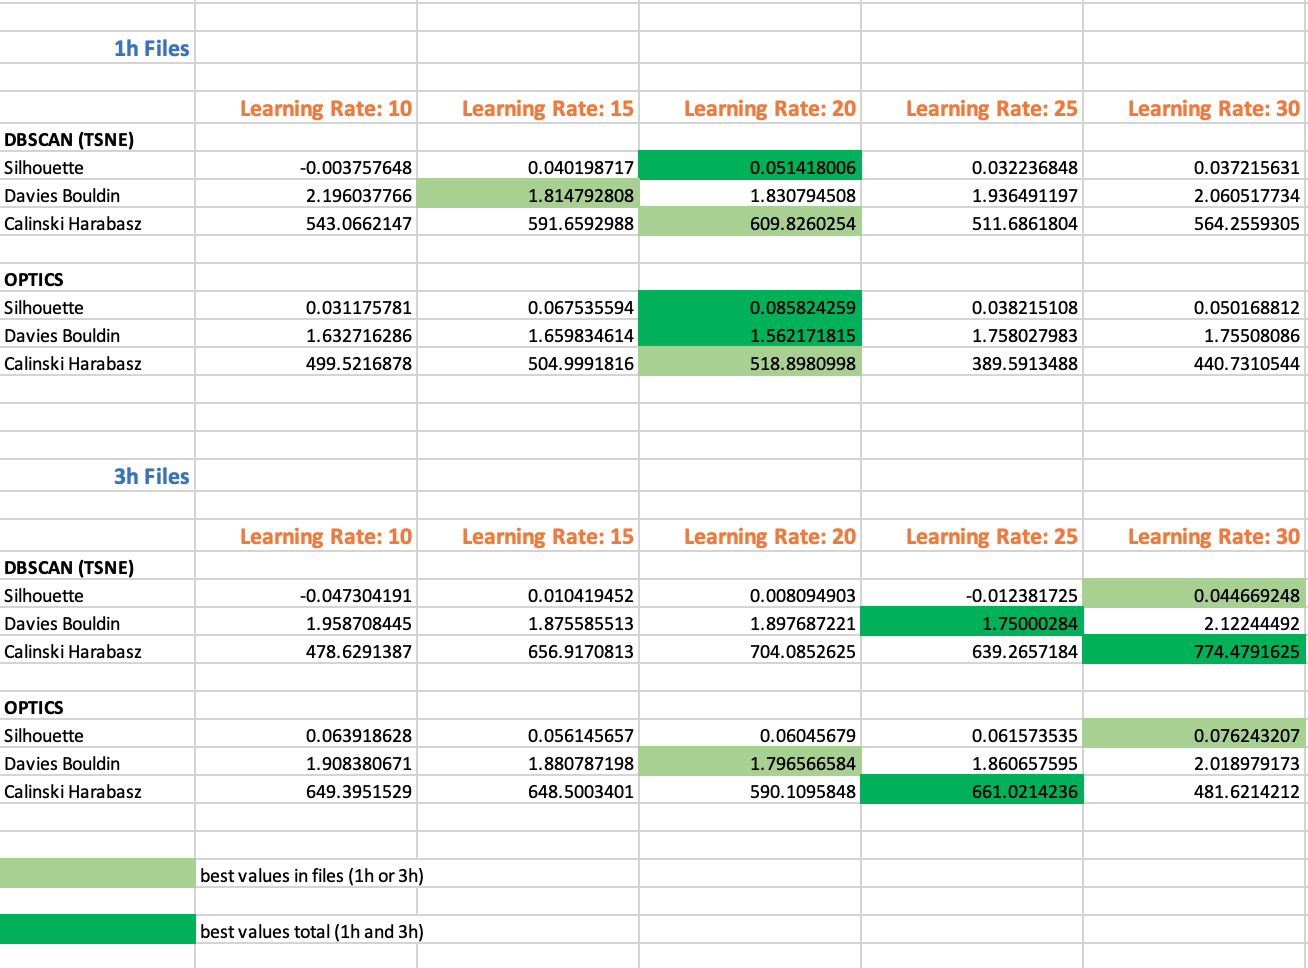
\includegraphics[width=0.8\textwidth]{./images/tsneParametersTest/learningRate/learningRateEvaluationScoresAverageDetailed3.png}
  \caption{Comparison of Silhouette Coefficient, Davies-Bouldin Index, and Caliński-Harabasz Index for different t-SNE \textbf{learning rate} values. The lighter green highlighted values indicate the best values of that file aggregation (1h or 3h files). The dark green highlighted values illustrate the overall best values over all files (1h and 3h files).}
  \label{figure:learningRateEvaluationScoresAverageDetailed3}
\end{figure}






\subsubsection{Learning Rate Comparison of 20 and 800}
\label{appendig:compareLearningRate20and800}

\begin{figure}[H]
  \centering
  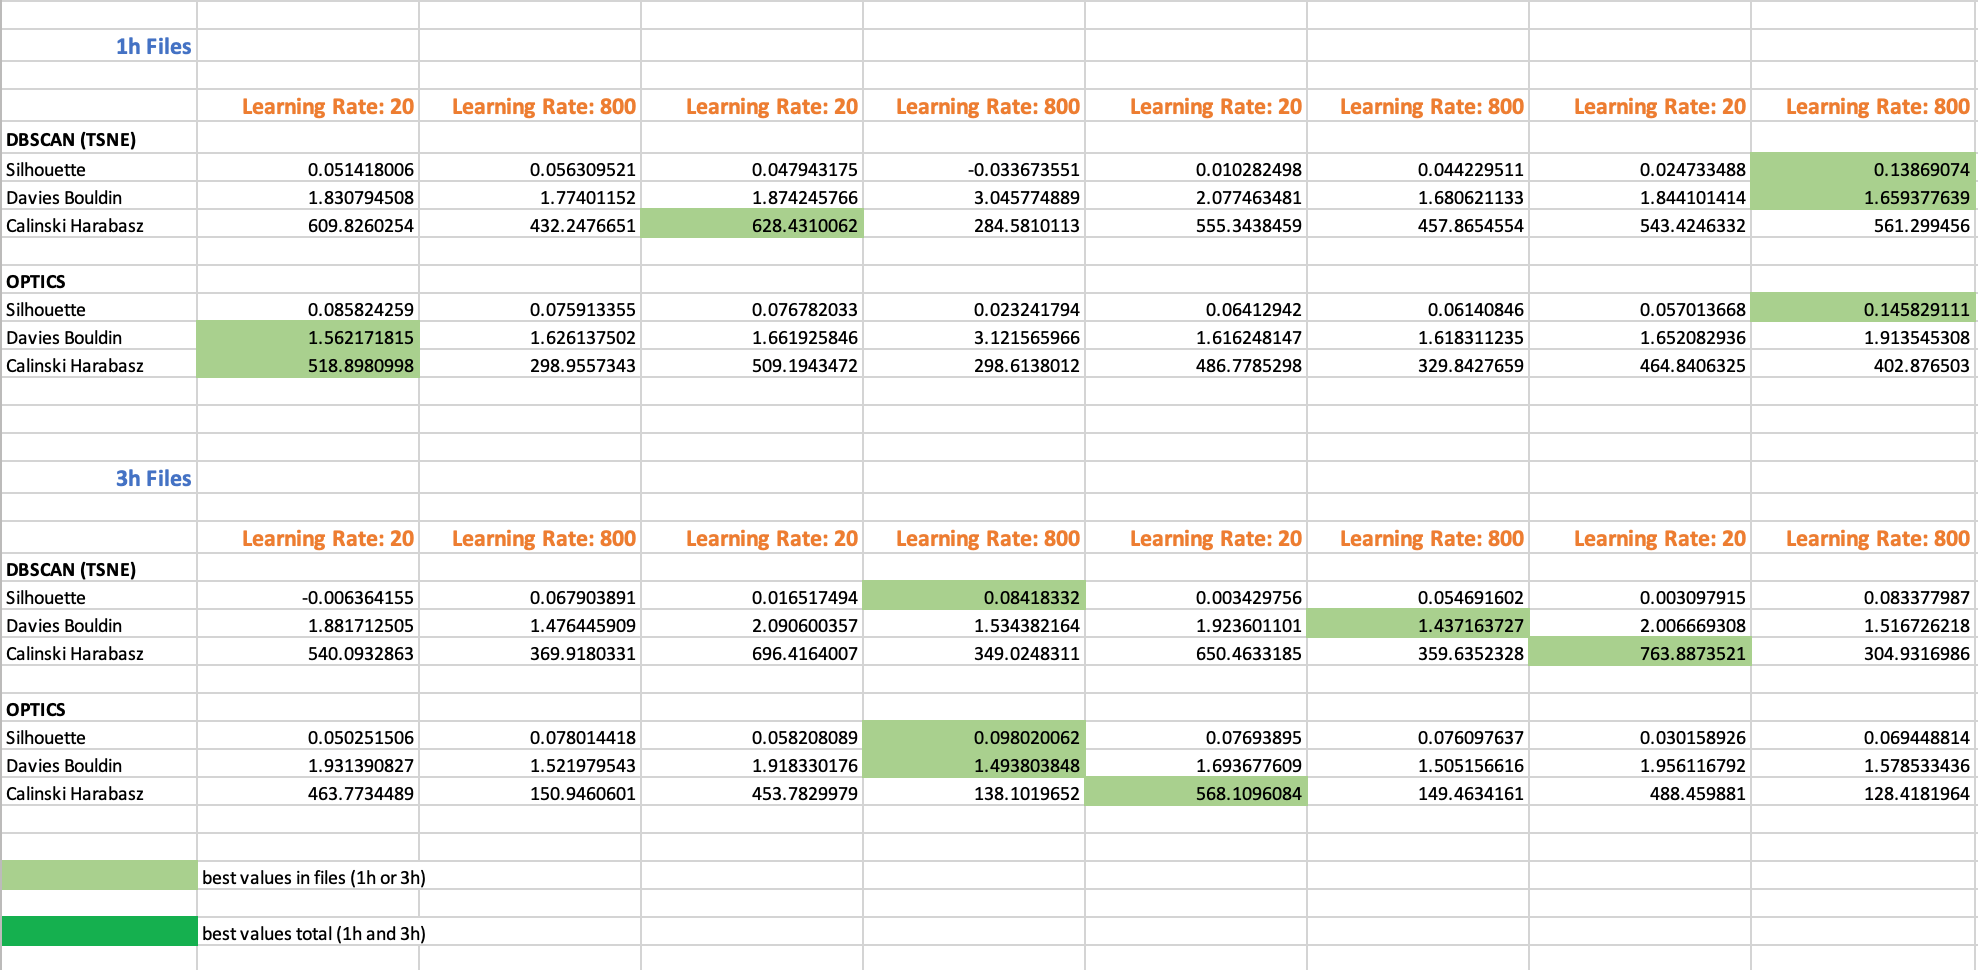
\includegraphics[width=1\textwidth]{./images/tsneParametersTest/learningRate/learningRateEvaluationScoresAverageDetailed4.png}
  \caption{Comparison of Silhouette Coefficient, Davies-Bouldin Index, and Caliński-Harabasz Index for the t-SNE \textbf{learning rate} values 20 and 80. The lighter green highlighted values indicate the best values of that file aggregation (1h or 3h files). The dark green highlighted values illustrate the overall best values over all files (1h and 3h files).}
  \label{figure:learningRateEvaluationScoresAverageDetailed4}
\end{figure}

%------------------ 1h: ------------------
\begin{figure}[H]
  \centering
  \begin{subfigure}{.5\textwidth}
    \centering
    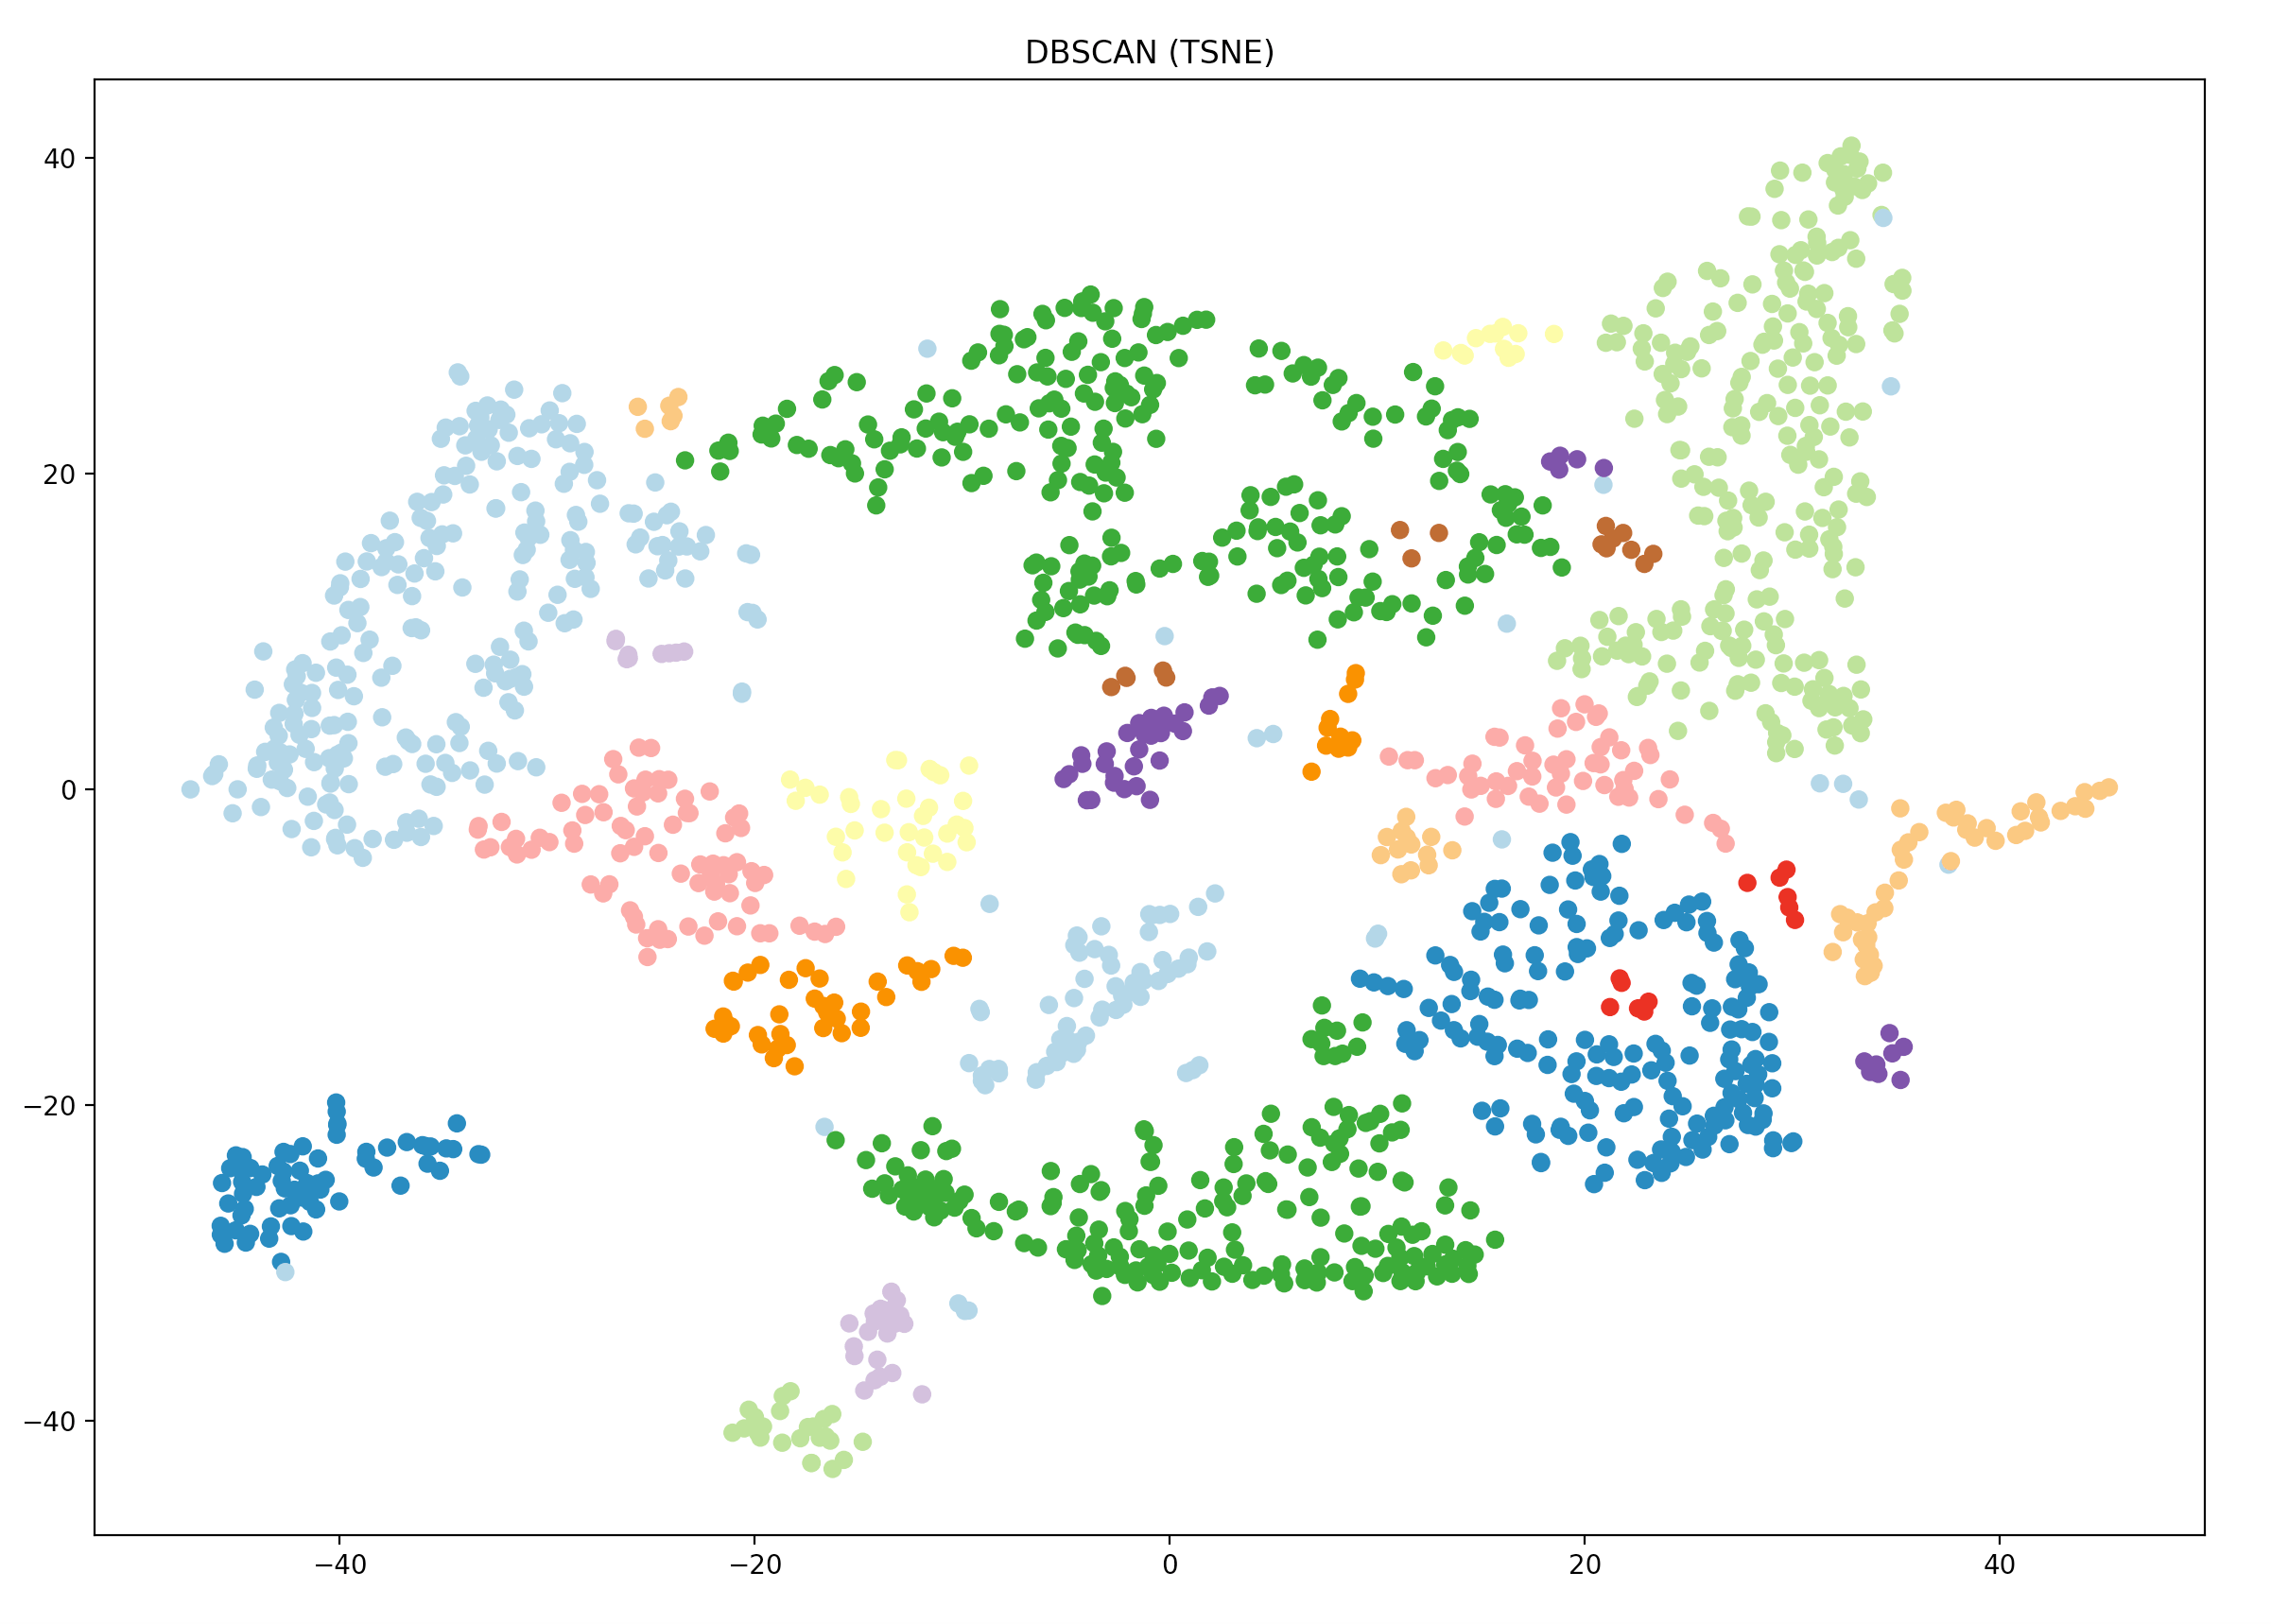
\includegraphics[width=0.9\textwidth]{./images/tsneParametersTest/learningRate/lr201h-DBSCANCompare.png}
  % \caption{}
  % \label{figure:}
  \end{subfigure}%
  \begin{subfigure}{.5\textwidth}
    \centering
    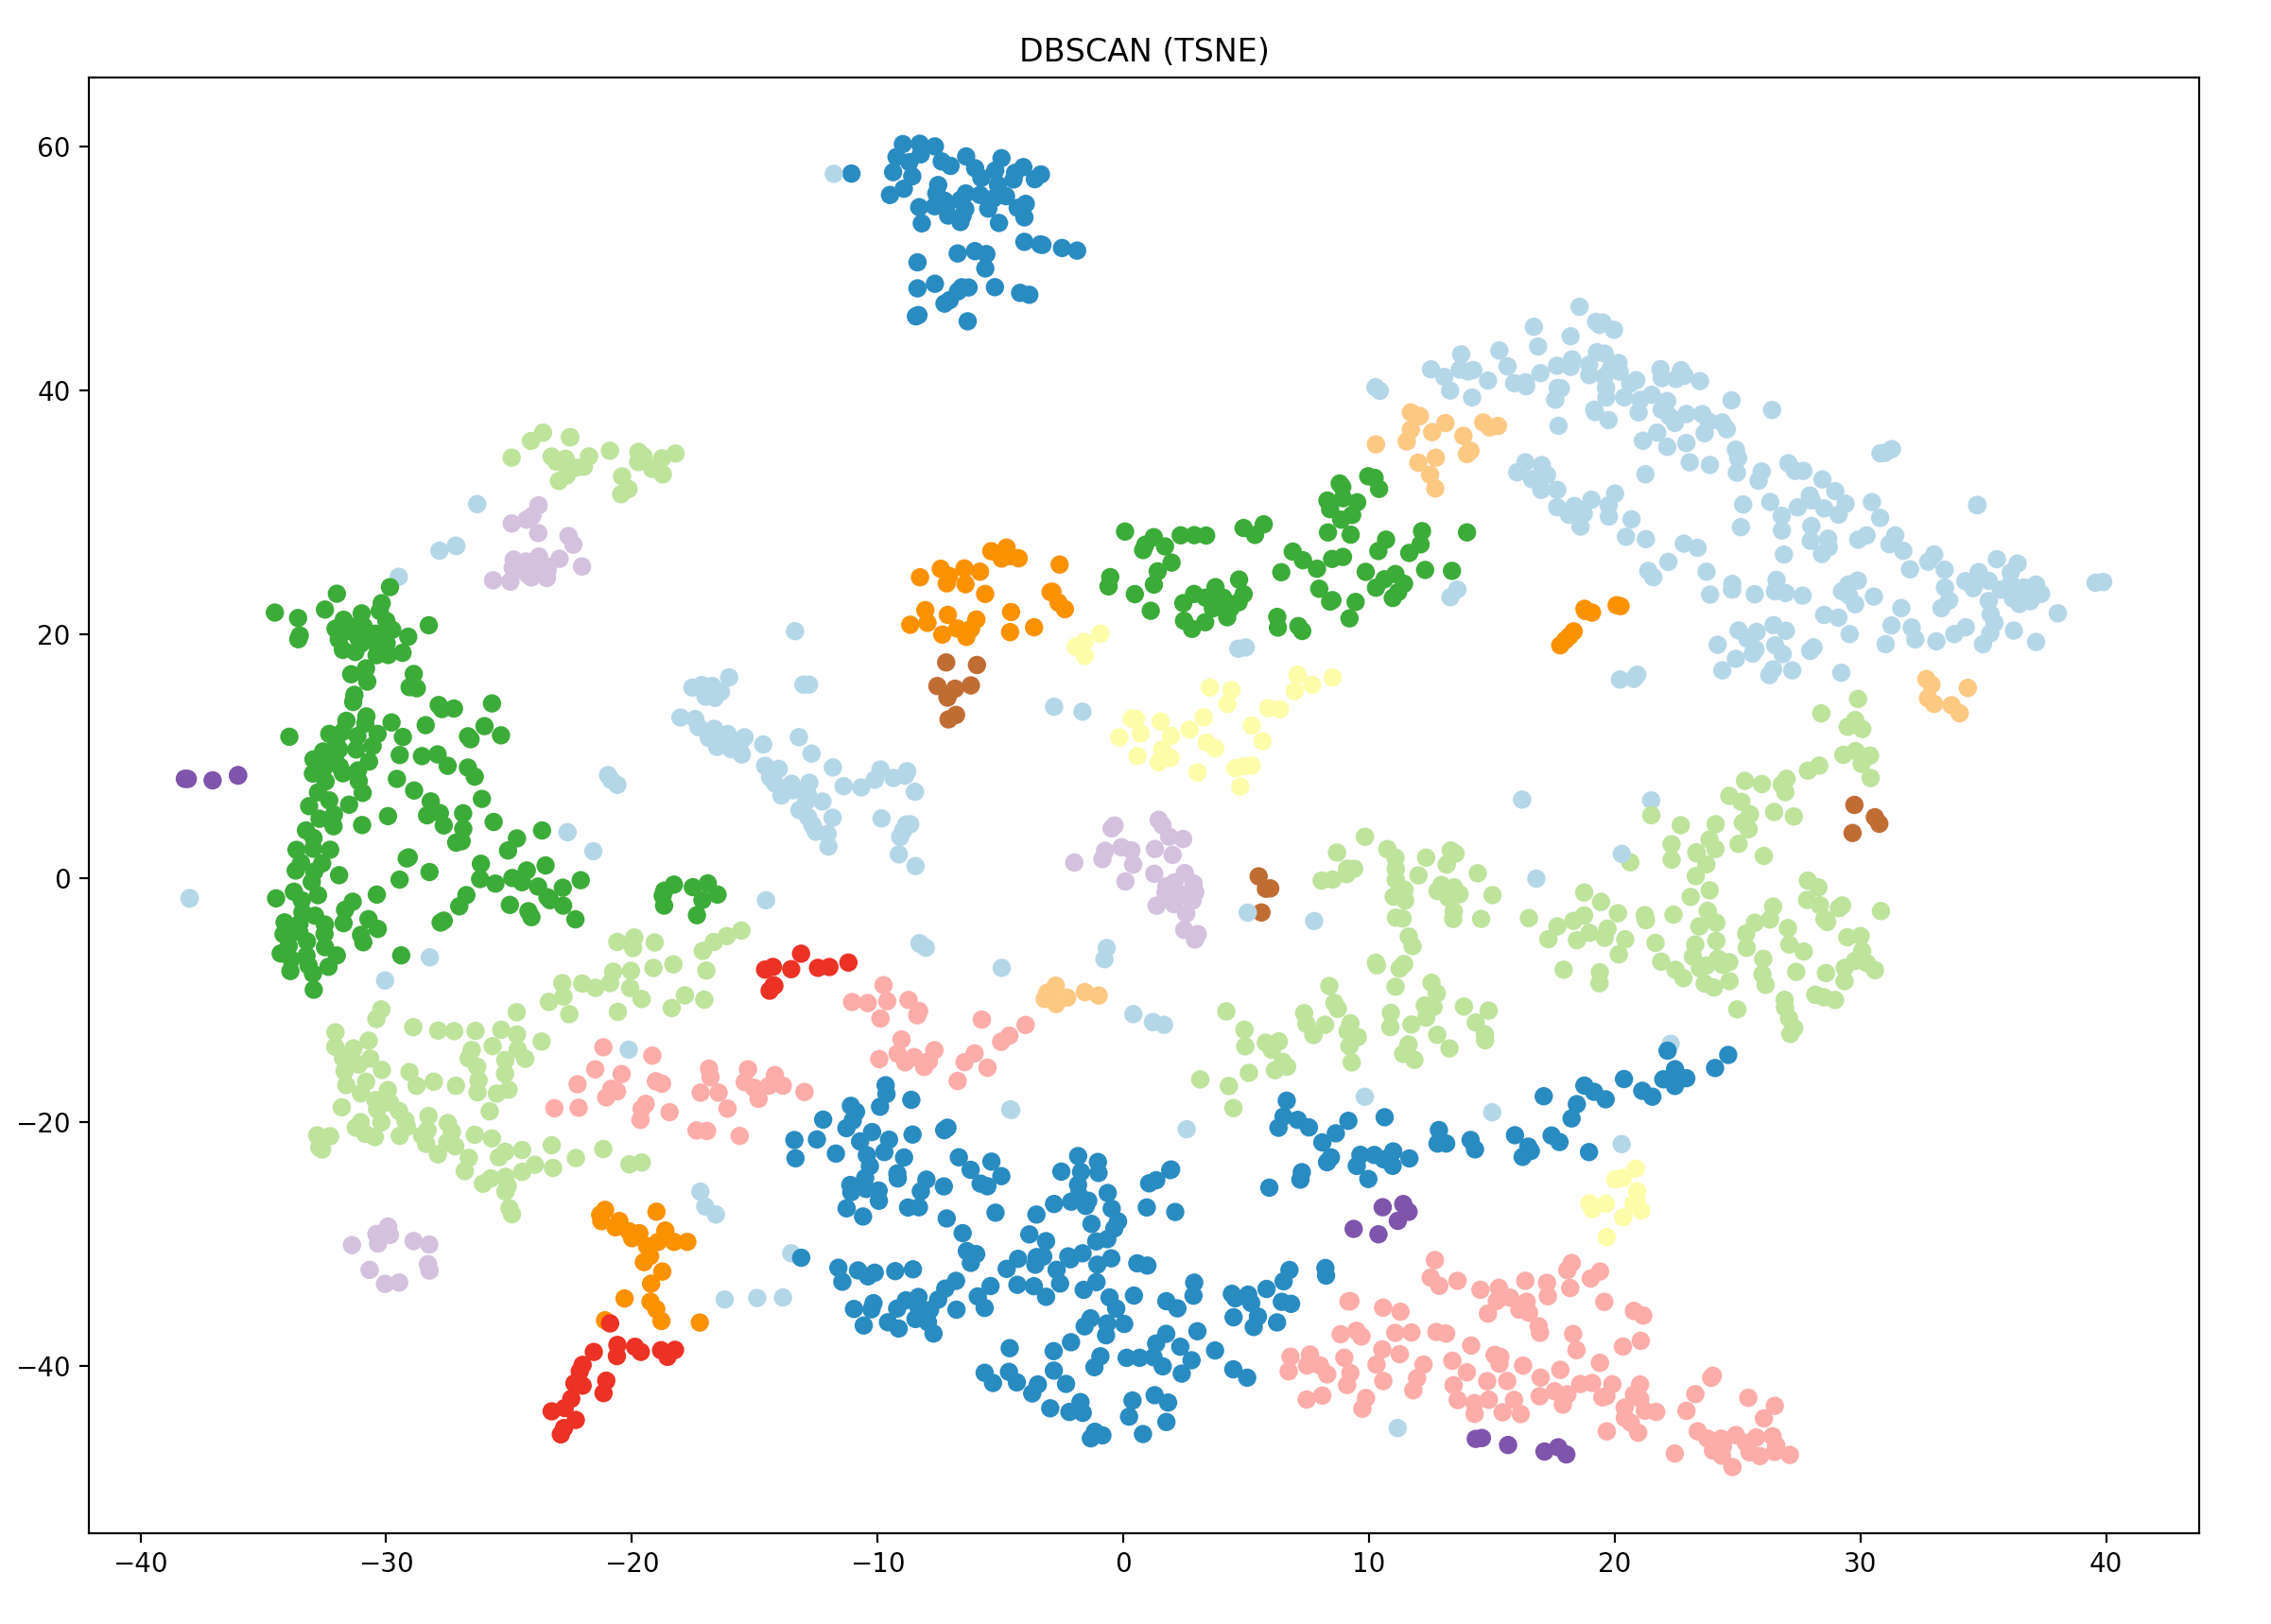
\includegraphics[width=0.9\textwidth]{./images/tsneParametersTest/learningRate/lr8001h-DBSCANCompare.png}
    % \caption{}
    % \label{figure:}
  \end{subfigure}
	\caption{\textbf{1h} data files comparison of learning rate: a) 20, b) 800}
	\label{figure:1h-learningRateComparison20and800}
\end{figure}
%------------------ 3h: ------------------
\begin{figure}[H]
  \centering
  \begin{subfigure}{.5\textwidth}
    \centering
    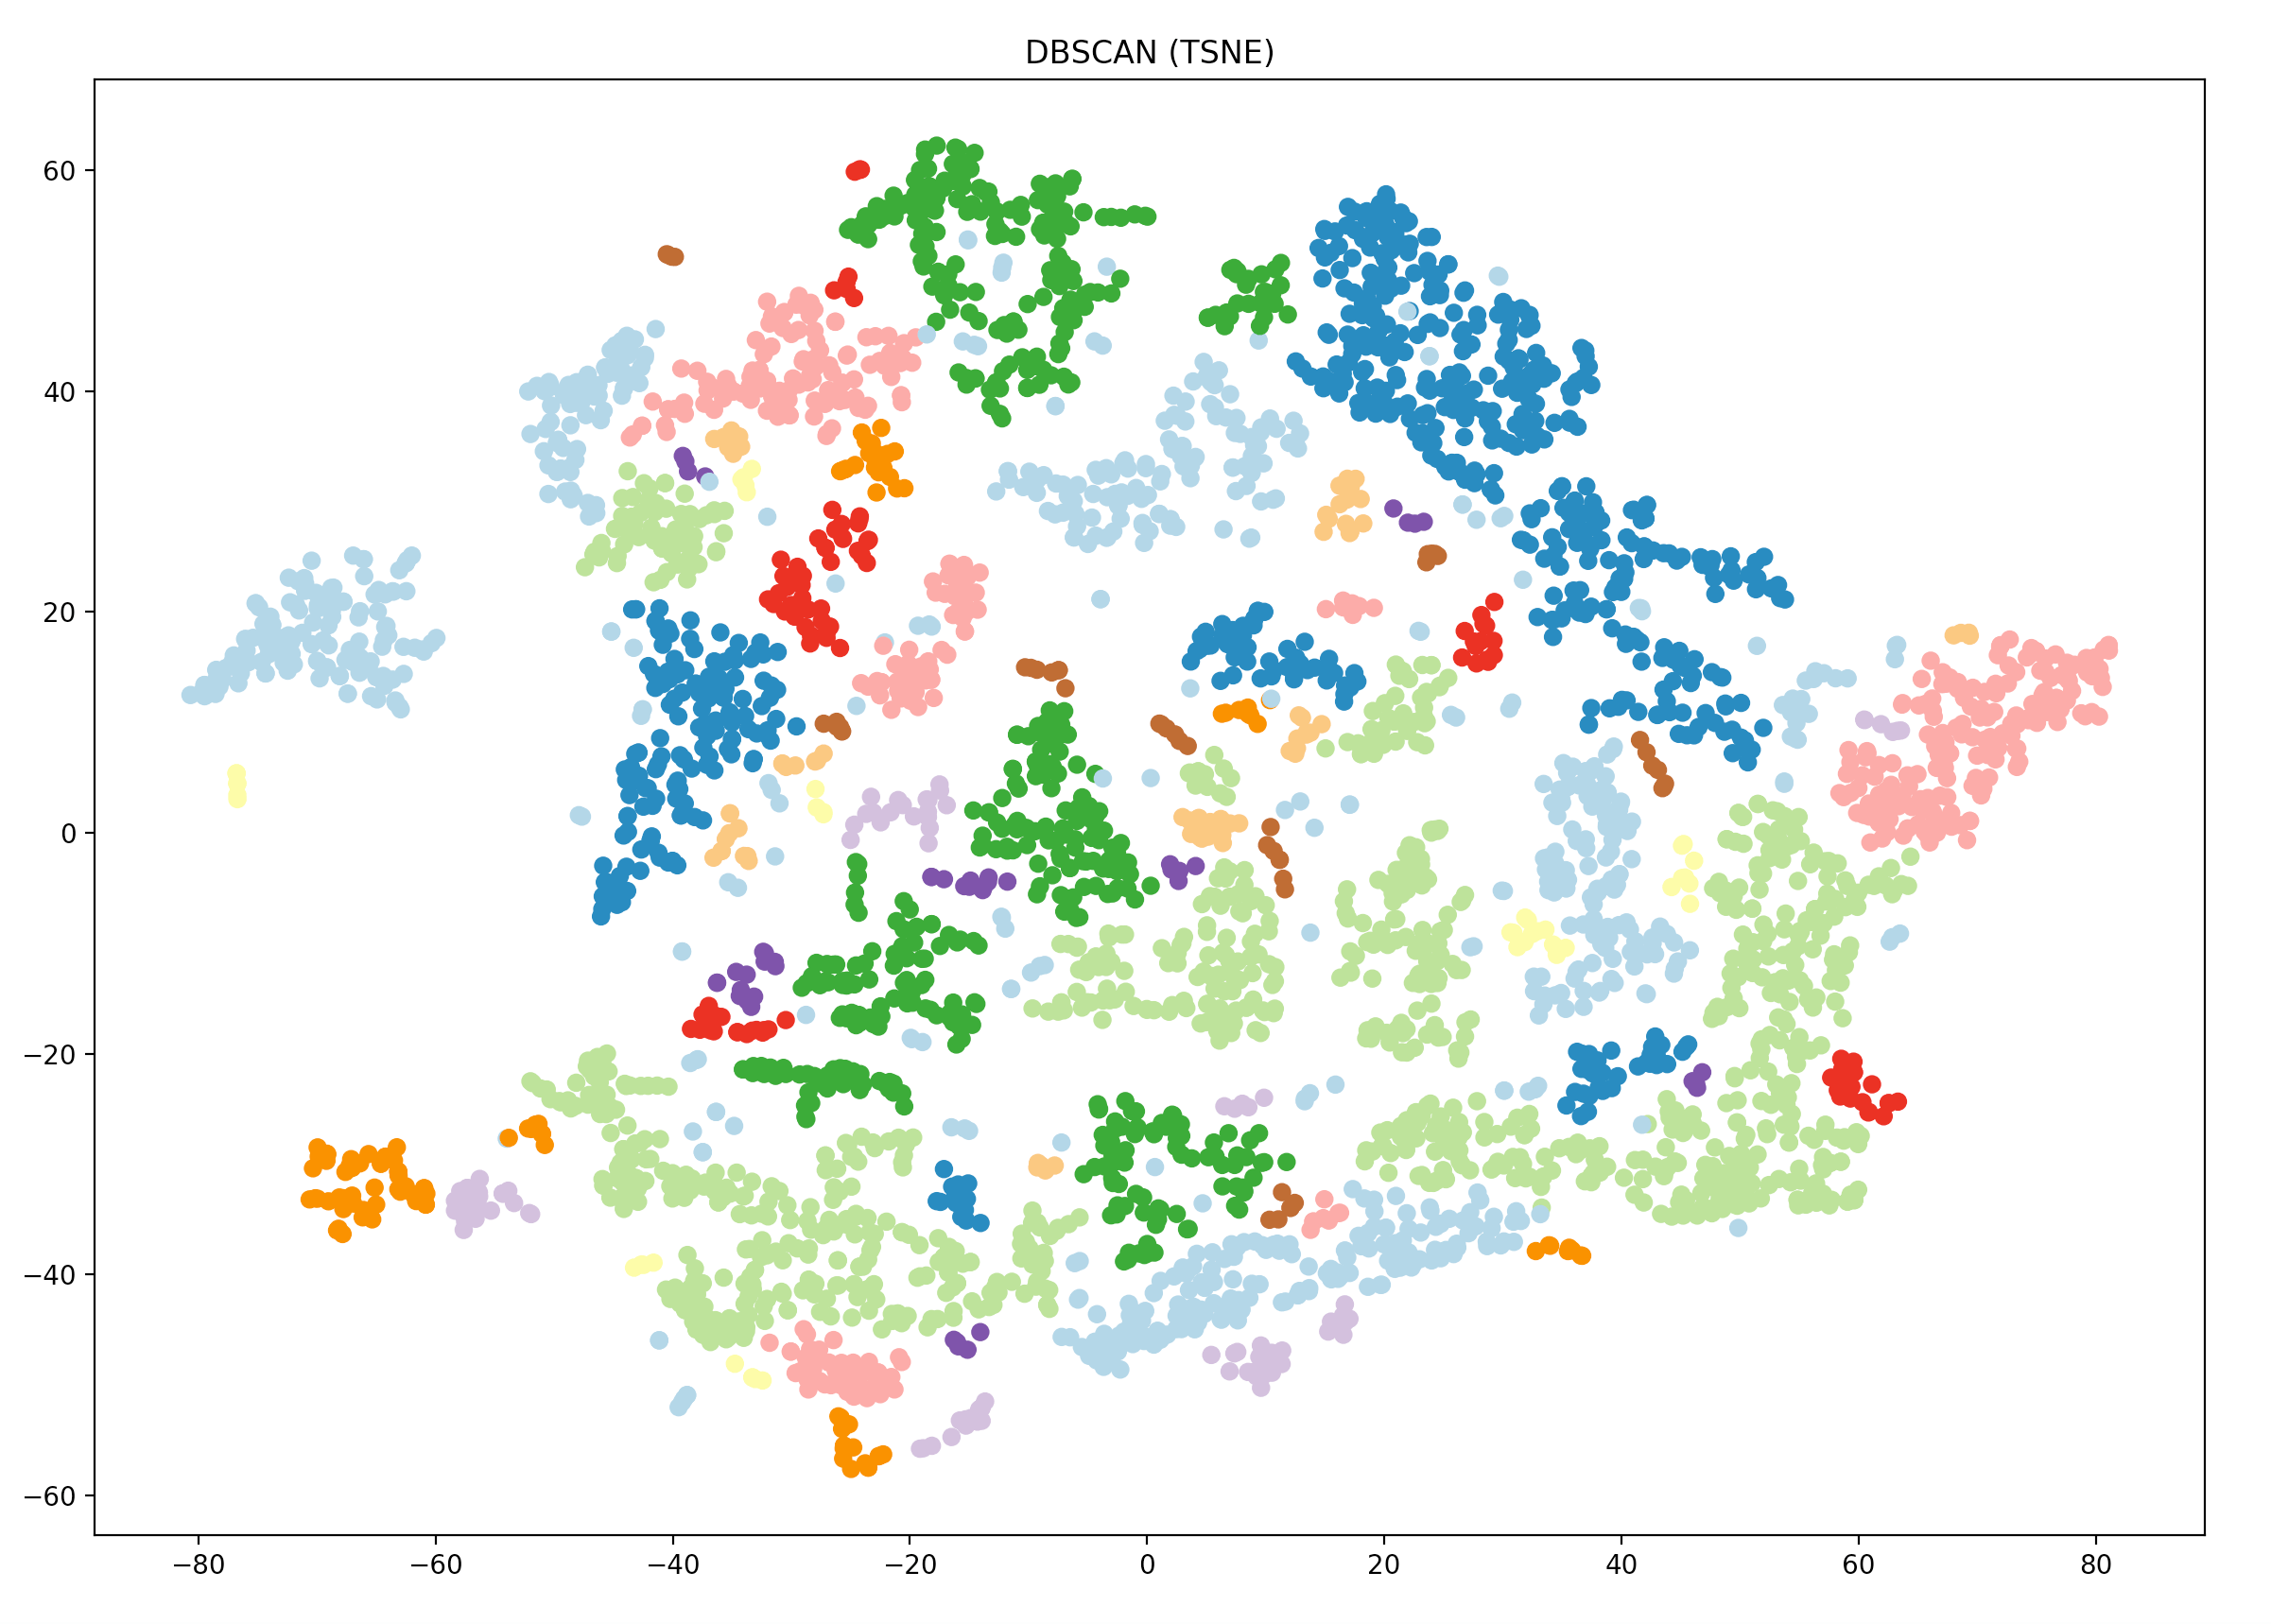
\includegraphics[width=0.9\textwidth]{./images/tsneParametersTest/learningRate/lr203h-DBSCANCompare.png}
  % \caption{}
  % \label{figure:}
  \end{subfigure}%
  \begin{subfigure}{.5\textwidth}
    \centering
    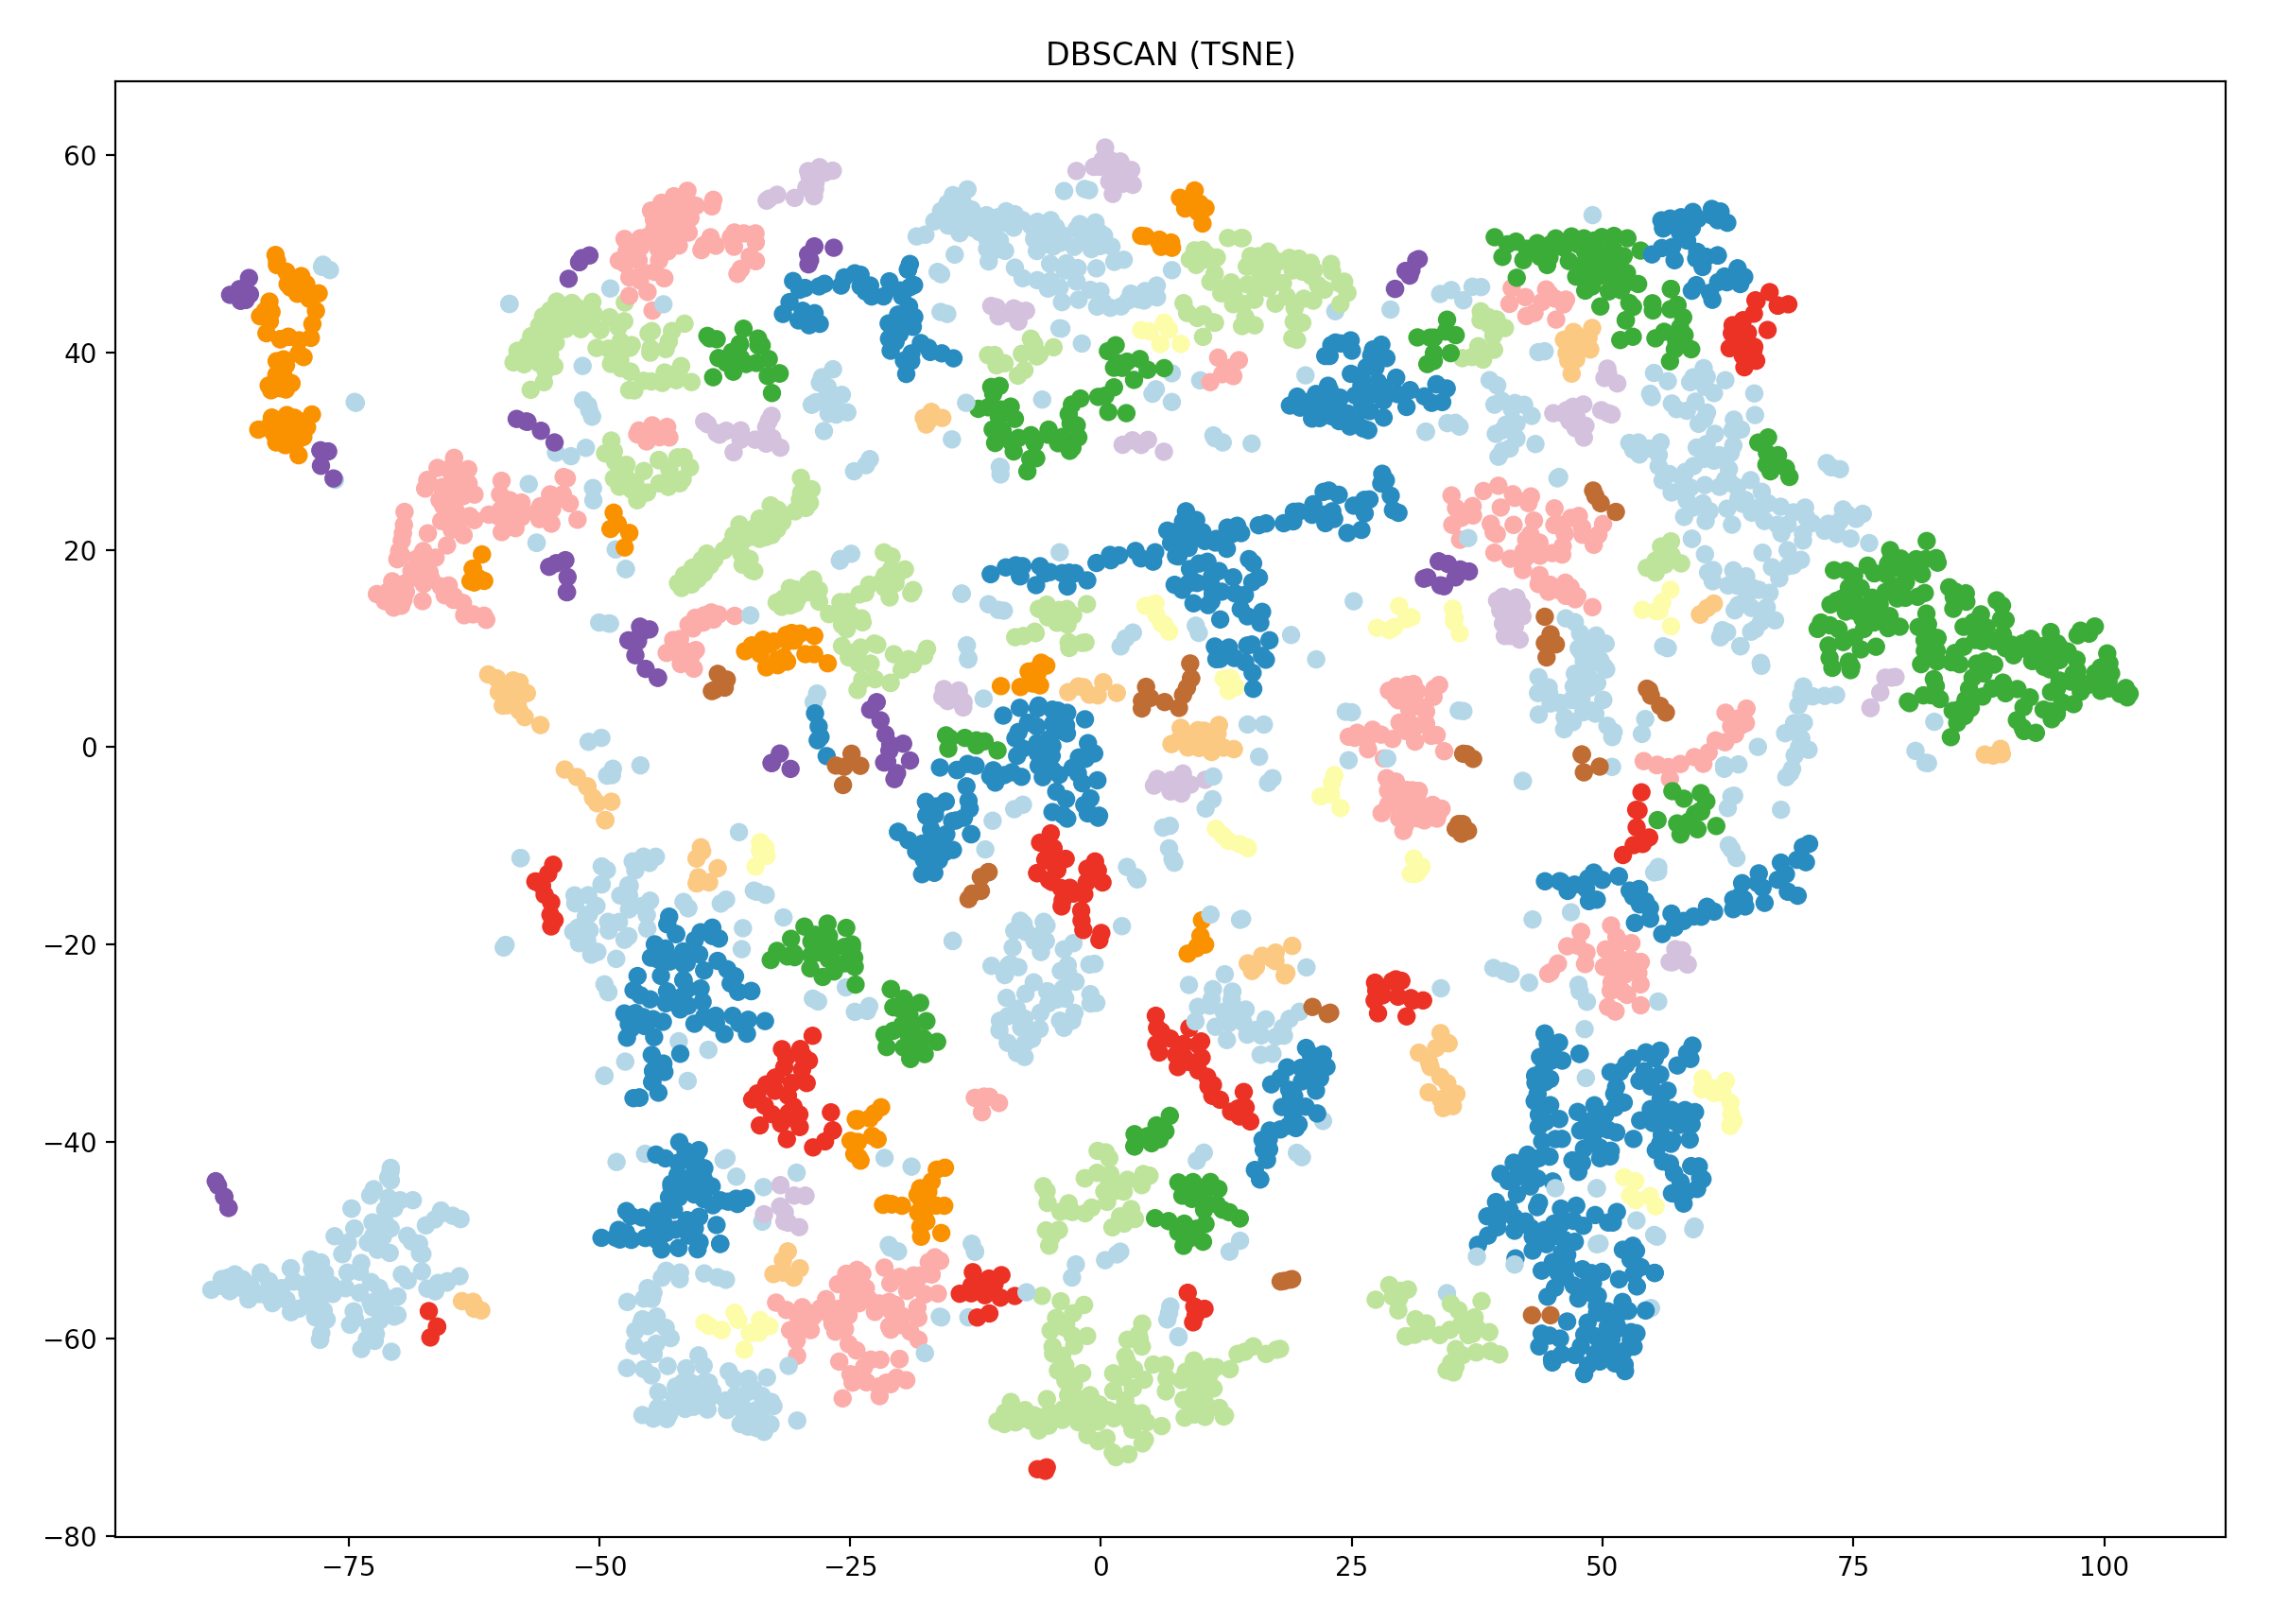
\includegraphics[width=0.9\textwidth]{./images/tsneParametersTest/learningRate/lr8003h-DBSCANCompare.png}
    % \caption{}
    % \label{figure:}
  \end{subfigure}
	\caption{\textbf{3h} data files comparison of learning rate: a) 20, b) 800}
	\label{figure:3h-learningRateComparison20and800}
\end{figure}


\clearpage